\documentclass[11pt,a4paper,oneside]{book}
\newcommand{\NumeroRelazione}{1}

\newcommand{\TitoloRelazione}{Misure su cavi coassiali, microstrisce e guide d'onda}
\usepackage[utf8]{inputenc}       
\usepackage[T1]{fontenc}          
\usepackage[italian]{babel}       
\usepackage{graphicx}             
\usepackage{float}
\usepackage{amsmath}
\usepackage{amsfonts} 
\usepackage{amssymb}  
\usepackage{steinmetz}
\usepackage{pgfplots}
\usepackage{tikz}
\usepackage{enumitem} 
\usepackage{subcaption}
\usepackage{caption}
\usepackage{comment}
\usepackage[normalem]{ulem}
\usepackage[americaninductors, siunitx]{circuitikz}

\usetikzlibrary{arrows.meta, patterns, shapes.geometric, calc, positioning, shapes, arrows}
\pgfplotsset{compat=1.18}

% --- GEOMETRY (Margini e distanze) ---
\usepackage[
    a4paper,
    top=3.5cm,      
    bottom=3cm,    
    left=3cm,      
    right=3cm,     
    headheight=40pt, % Spazio per l'immagine
    headsep=25pt     % Distanza tra immagine e testo/titoli
]{geometry}

% --- FANCYHDR (Intestazioni) ---
\usepackage{fancyhdr} 
\pagestyle{fancy}
\fancyhf{} 
\fancyhead[L]{
\includegraphics[height=1cm]{Images/top.png}} 
\fancyhead[R]{\thepage} 
\fancyhead[C]{\textit{\leftmark}} 

% Per avere l'intestazione anche nelle pagine iniziali dei capitoli
\fancypagestyle{plain}{
  \fancyhf{}
  \fancyhead[L]{
\includegraphics[height=1cm]{Images/top.png}}
  \fancyhead[R]{\thepage}
  \fancyhead[C]{\textit{\leftmark}}
  \renewcommand{\headrulewidth}{0.4pt}
}

% --- LINK CLICCABILI (Senza il backtick d'errore) ---
\usepackage[hidelinks]{hyperref} 
 

% --- COMANDI PERSONALIZZATI ---
\newcommand{\tikznode}[2]{%
  \ifmmode%
    \tikz[remember picture,baseline=(#1.base),inner sep=0pt] \node (#1) {$#2$};%
  \else
    \tikz[remember picture,baseline=(#1.base),inner sep=0pt] \node (#1) {#2};%
  \fi%
}
\tikzset{portnode/.style={circle, draw, inner sep=1pt, font=\scriptsize}}


\begin{document}
% --- PAGINA DEL TITOLO 
\begin{titlepage}
    \centering
    {\scshape\Large Università degli Studi "La Sapienza" \par} 
    \vspace{0.5cm}
    {\scshape\large Dipartimento di Ingegneria dell'Informazione, Elettronica e Telecomunicazioni \par}
    \vspace{0.5cm}
    {\scshape\large Corso di Laurea in Ingegneria Elettronica \par}
    \vspace{1.5cm}
    {\huge\bfseries Laboratorio Multidisciplinare\\ di Elettronica I\par}
    \vspace{0.35cm}
    {\Large\bfseries Relazione \NumeroRelazione\par}
    \vspace{0.35cm}
    {\Large\bfseries \TitoloRelazione\par}
    \vspace{1cm}
    {\large CFU:  6 \par} 
    \vspace{2.5cm}

    {\large Gruppo 18: \par}
    \vspace{0.2cm}
    {\Large Renato Bearzotti \par}
    {\Large Nicolò Falasca \par}

    \vspace{0.8cm}
    \IfFileExists{Images/top.png}{%
        
\includegraphics[width=3.5cm]{Images/top.png}\par
    }{}
    \vspace{0.35cm}
    \IfFileExists{Images/logo Sapienza (rgb).png}{%
        
\includegraphics[width=6.8cm]{Images/logo Sapienza (rgb).png}\par
    }{}
    \vspace{0.8cm}

    % Professori allineati a destra
    \begin{minipage}[t]{\textwidth}
        \begin{flushright}
            \large
            \textbf{Professori:}\\
            Andrea Mostacci\\
            Stefano Pisa\\
            Pasquale Tommasino
        \end{flushright}
    \end{minipage}

    \vfill
    {\large Anno Accademico 2026-2027 \par}
\end{titlepage}


\frontmatter 
\tableofcontents

\mainmatter



% =====================================================================
% PUNTI 1-3 (Renato). Figure in Images/Relazione1_Foto/, fatte in MATLAB
% dai file .mat del banco (script p1_verifica_calibrazione.m,
% p2_attenuazione_marker.m, p3_fit_sqrtf.m nella cartella Dati_e_routine).
% =====================================================================
% Capitolo 1
% =====================================================================
\chapter{Calibrazione del VNA e sua verifica}
Per prima cosa abbiamo calibrato l'analizzatore di reti vettoriale (VNA, versione USB) con una calibrazione \emph{Full 2-Port} nella banda da 300\,kHz a 1.5\,GHz e di acquisire, salvare e graficare i risultati della calibrazione, cioè tre verifiche:
\begin{itemize}
  \item il modulo in dB di $S_{11}$ del carico adattato da 50\,$\Omega$, su carta rettangolare (formato Log Mag);
  \item $S_{11}$ del corto circuito sulla carta di Smith;
  \item il modulo in dB di $S_{21}$ con la porta 1 collegata alla porta 2 (\emph{thru}), su carta rettangolare.
\end{itemize}

\section{Modello d'errore del VNA e risposta attesa}
Il VNA non misura direttamente i parametri $S$ del dispositivo: fra i ricevitori e il dispositivo ci sono accoppiatori, cavi e connettori, i cui errori sistematici sono descritti dal modello a 12 termini (direttività, adattamento di sorgente e di carico, tracking in riflessione e in trasmissione, isolamento, per ciascuna delle due direzioni). La calibrazione misura degli standard noti, ricava i termini d'errore e da quel momento li toglie da ogni misura; il piano di riferimento diventa l'estremità dei due cavi di misura. Se la calibrazione funziona, misurando oggetti di cui conosciamo la risposta dobbiamo ritrovare la risposta ideale:
\begin{itemize}
  \item \textbf{carico adattato}: $S_{11} = 0$, cioè $|S_{11}|_{dB}\to-\infty$; in pratica un valore molto basso;
  \item \textbf{corto}: $S_{11} = -1$, cioè $|S_{11}| = 0$\,dB e un punto sul bordo della carta di Smith. Se il corto non è esattamente sul piano di riferimento ma dietro un breve tratto di linea, la traccia resta sul bordo e ruota in senso orario al crescere della frequenza;
  \item \textbf{thru}: $S_{21} = 1$, cioè $|S_{21}| = 0$\,dB. Per collegare fra loro i due cavi serve un raccordo, che non è un thru ideale di lunghezza nulla: aggiunge un piccolo ritardo.
\end{itemize}
Quello che si misura in più rispetto alla risposta ideale è l'errore residuo dopo la correzione. Al primo ordine nei termini d'errore residui (direttività $D$, adattamento di sorgente $M_S$ e di carico $M_L$, tracking in riflessione $F_R$ e in trasmissione $F_T$, isolamento $C$)
\begin{align}
\Delta_{11} = S_{11,m}-S_{11} &\simeq D + (F_R-1)\,S_{11} + M_L\,S_{12}S_{21} + M_S\,S_{11}^2, \\
\Delta_{21} = S_{21,m}-S_{21} &\simeq C + (F_T-1)\,S_{21} + M_S\,S_{21}S_{11} + M_L\,S_{21}S_{22}.
\end{align}
Quindi il carico ($S_{11} = 0$) misura la direttività residua, il corto ($S_{11} = -1$) soprattutto il tracking in riflessione e l'adattamento di sorgente residui, il thru ($S_{21} = 1$, porte adattate) il tracking residuo in trasmissione. Le tre verifiche ci dicono quindi anche quale incertezza attribuire alle misure successive.

\section{Strumento e calibrazione}
L'analizzatore è un Keysight P9372A con interfaccia USB, comandato dal PC del banco. Le tracce sono state acquisite con 
la routine del corso \texttt{DataAquisition11.m}, che salva la struttura \texttt{dataStruct}
con le frequenze, il parametro $S$ complesso e il dato nel formato dello schermo. 
La calibrazione Full 2-Port da 300\,kHz a 1.5\,GHz era già attiva all'inizio del turno: 
lo si vedeva dalla banda indicata sullo schermo, e il file salvato dallo strumento 
(\texttt{300K\_1500M\_2PORT\_10\_22\_26.csa}) riporta che è stata eseguita alle 13:01 del
22 ottobre con il calibratore elettronico (ECal) N4691-60006. Dallo stesso file si leggono
le impostazioni, comuni a tutte le misure dei punti 1--3: 1601 punti (passo 0.9373\,MHz),
banda IF 2\,kHz, potenza $-5$\,dBm su entrambe le porte. Il termine di isolamento nel
file è nullo ($-313$\,dB): la calibrazione è stata fatta senza la misura di isolamento.

\section{Carico adattato}
\begin{figure}[H]
    \centering
    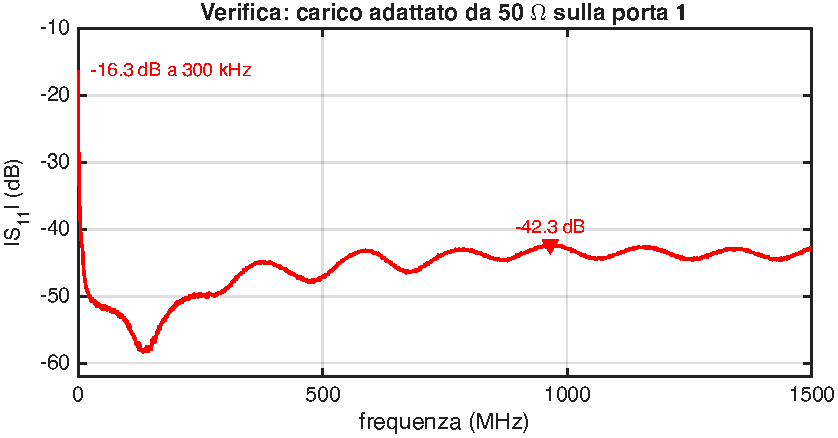
\includegraphics[width=0.9\textwidth]{Images/Relazione1_Foto/p1_carico.pdf}
    \caption{Carico adattato da 50\,$\Omega$ sulla porta 1: modulo di $S_{11}$ in dB.}
    \label{fig:p1carico}
\end{figure}
Da 10\,MHz in su $|S_{11}|\le-42.3$\,dB (il massimo è a 966\,MHz, la mediana è $-44.4$\,dB), cioè un coefficiente di riflessione residuo $|\Gamma|\le0.0077$ (fig.~\ref{fig:p1carico}). Questo valore comprende sia la riflessione del carico stesso sia l'errore residuo dello strumento: la calibrazione funziona. Fa eccezione l'estremo basso della banda: il primo punto (300\,kHz) vale $-16.3$\,dB e la traccia scende sotto $-40$\,dB solo da 5.9\,MHz in su. Nel file di calibrazione la direttività \emph{non corretta} dello strumento a 300\,kHz è solo $-7.7$\,dB, contro valori fra $-31$ e $-44$\,dB nel resto della banda: lì la correzione è molto sensibile a qualunque piccola variazione avvenuta dopo la calibrazione (cavi mossi, ripetibilità dei connettori). I primissimi punti della banda vanno quindi presi con cautela anche nelle misure successive.

\section{Corto}
\begin{figure}[H]
    \centering
    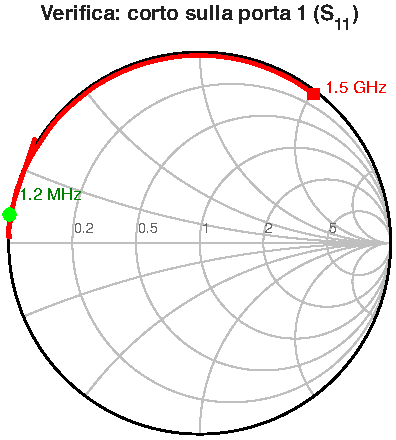
\includegraphics[width=0.5\textwidth]{Images/Relazione1_Foto/p1_corto.pdf}
    \caption{Corto circuito sulla porta 1: $S_{11}$ sulla carta di Smith, dal marker verde (1.2\,MHz) a quello rosso (1.5\,GHz).}
    \label{fig:p1corto}
\end{figure}
La traccia sta sul bordo della carta di Smith (fig.~\ref{fig:p1corto}): da 10\,MHz in su $|S_{11}|$ è compreso fra $-0.17$ e $+0.02$\,dB, come deve essere per un carico puramente reattivo. La fase non resta a $180^\circ$ ma ruota in senso orario, linearmente con la frequenza, fino a $52.6^\circ$ a 1.5\,GHz: la regressione lineare della fase dà una pendenza di $-8.437\cdot10^{-8}$\,gradi/Hz e un'intercetta di $179.1^\circ$, quasi $180^\circ$ a frequenza nulla. Come per il carico, fanno eccezione i primissimi punti: a 300\,kHz la fase vale $147^\circ$ e $|S_{11}| = +0.20$\,dB, valore impossibile per un corto passivo, e a 1.2\,MHz (marker verde) la fase vale $171.5^\circ$ invece di $179^\circ$; da 10\,MHz in su i punti stanno sulla retta entro $1^\circ$. È il comportamento di un corto posto dietro un breve tratto di linea,
\begin{equation}
S_{11} = -\mathrm{e}^{-\mathrm{j}\omega\,2\tau_c}, \qquad \tau_c = \frac{8.437\cdot10^{-8}\ \mathrm{gradi/Hz}}{2\cdot360^\circ} = 117\ \mathrm{ps}\quad(3.5\ \mathrm{cm\ in\ aria}),
\end{equation}
quindi il corto usato non si trova esattamente sul piano di riferimento della calibrazione. La piccola perdita che compare verso 1.5\,GHz (fino a $-0.17$\,dB) comprende quella di questo tratto, percorso in andata e ritorno, e l'errore residuo dello strumento in riflessione.

\section{Thru}
\begin{figure}[H]
    \centering
    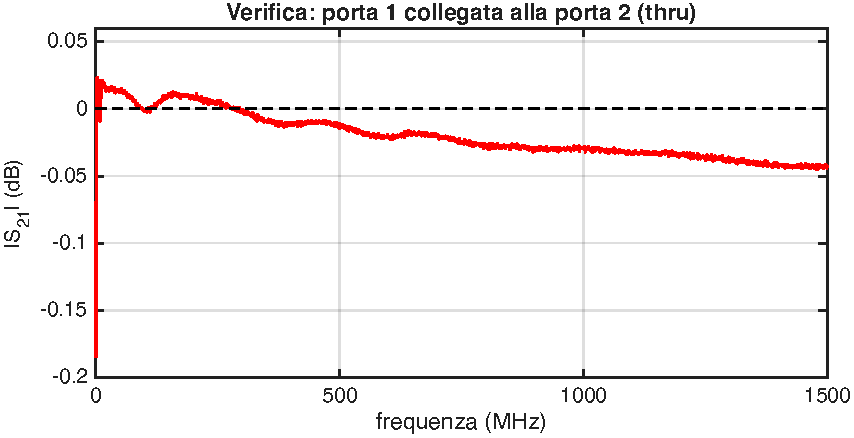
\includegraphics[width=0.9\textwidth]{Images/Relazione1_Foto/p1_thru.pdf}
    \caption{Porta 1 collegata alla porta 2 con un raccordo (thru): modulo di $S_{21}$ in dB.}
    \label{fig:p1thru}
\end{figure}
Con le due porte collegate da un raccordo, da 1\,MHz in su $|S_{21}|$ resta fra $-0.045$ e $+0.023$\,dB (media $-0.020$\,dB, deviazione standard 0.017\,dB); solo il primo punto (300\,kHz) vale $-0.185$\,dB (fig.~\ref{fig:p1thru}). La fase di $S_{21}$ scende linearmente con la frequenza, con pendenza di $-3.064\cdot10^{-8}$\,gradi/Hz: corrisponde a un ritardo di 85\,ps (2.5\,cm in aria), quello del raccordo. Lo scostamento da 0\,dB cresce lentamente con la frequenza e comprende anche la piccola perdita del raccordo: come stima dell'errore residuo dello strumento in trasmissione è quindi per eccesso.

\section{Errori residui e incertezze per i punti successivi}
\begin{table}[H]
\centering
\caption{Risultati della verifica della calibrazione (da 10\,MHz in su per il carico e il corto, da 1\,MHz in su per il thru).}
\label{tab:p1}
\begin{tabular}{l|c|c|c}
\hline
verifica & atteso & misurato & errore residuo \\ \hline
carico 50\,$\Omega$ & $|S_{11}|\to-\infty$ & $|S_{11}|\le-42.3$\,dB & $|\Gamma|\le0.0077$ \\
corto & $|S_{11}| = 0$\,dB & da $-0.17$ a $+0.02$\,dB & sul bordo della carta \\
thru & $|S_{21}| = 0$\,dB & da $-0.045$ a $+0.023$\,dB & $\pm0.045$\,dB \\ \hline
\end{tabular}
\end{table}
Le tre verifiche danno il risultato atteso in tutta la banda, con l'avvertenza sui primi punti sotto qualche MHz (tab.~\ref{tab:p1}). Non avendo altre informazioni sull'accuratezza dello strumento, usiamo questi errori residui come limiti di distribuzioni rettangolari: per i moduli misurati in trasmissione $u = 0.045/\sqrt3 = 0.026$\,dB (punto~2); per i coefficienti di riflessione $u = 0.0077/\sqrt3 = 0.0044$ sulla parte reale e su quella immaginaria. Tutte le incertezze di questi tre punti sono incertezze tipo ($k = 1$); nei risultati dei punti 2 e 3 sono arrotondate per eccesso a due cifre significative.

% =====================================================================
% Capitolo 2
% =====================================================================
\chapter{Attenuazione del cavo coassiale con il marker}
Sul banco c'è un cavo coassiale di lunghezza fisica $L = 10$\,m (dato della practice). Lo si collega fra le due porte del VNA, si misura $S_{21}(f)$ in formato Log Mag su carta rettangolare e si legge con un marker l'attenuazione del cavo a $f = 750$\,MHz.

\section{Attenuazione attesa}
Il cavo è da 50\,$\Omega$ ed è chiuso su porte da 50\,$\Omega$: non ci sono riflessioni apprezzabili e $S_{21}$ è il solo termine di propagazione,
\begin{equation}
S_{21}(\omega) = \mathrm{e}^{-\gamma L} = \mathrm{e}^{-\alpha L}\,\mathrm{e}^{-\mathrm{j}\beta L},
\qquad A = -|S_{21}|_{dB} = 8.686\,\alpha L ,
\end{equation}
dove $8.686 = 20\log_{10}\mathrm{e}$ converte i neper in decibel. Nei cavi dominano le perdite nei conduttori, che per effetto pelle crescono con la radice della frequenza: $\alpha = \alpha'\sqrt\omega$. Ci aspettiamo quindi:
\begin{itemize}
  \item una curva che parte da 0\,dB a frequenza nulla con tangente verticale (la derivata di $\sqrt f$ diverge nell'origine) e poi scende sempre più lentamente;
  \item nessuna ondulazione apprezzabile, perché il cavo è adattato alle porte;
  \item come ordine di grandezza, l'esempio visto a lezione di un tipico cavo RG58, $\alpha\simeq0.04$\,m$^{-1}$ a 1\,GHz (circa 0.35\,dB/m): scalando come $\sqrt f$, 10\,m a 750\,MHz darebbero circa 3\,dB. Il nostro cavo non è necessariamente un RG58: il numero serve solo a sapere che cosa aspettarsi.
\end{itemize}

\section{Misura dell'attenuazione a 750\,MHz}
\begin{figure}[H]
    \centering
    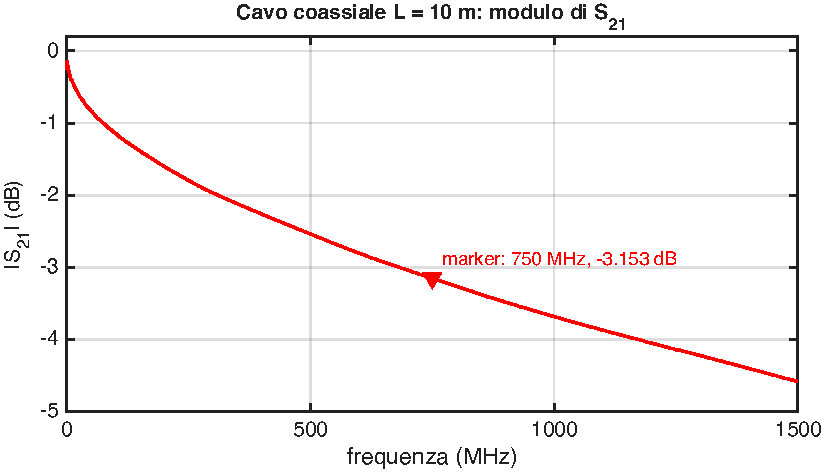
\includegraphics[width=0.9\textwidth]{Images/Relazione1_Foto/p2_S21_cavo.pdf}
    \caption{Cavo coassiale da 10\,m fra le due porte: modulo di $S_{21}$ in dB, con il marker a 750\,MHz.}
    \label{fig:p2}
\end{figure}
La traccia (fig.~\ref{fig:p2}) ha l'andamento atteso: scende rapidamente alle frequenze più basse e poi sempre più lentamente, fino a $-4.58$\,dB a 1.5\,GHz, senza ondulazioni visibili (le irregolarità da un punto all'altro sono di qualche millesimo di dB). Fa eccezione il primo punto, a 300\,kHz: vale $-0.26$\,dB, mentre scalando come $\sqrt f$ il valore a 750\,MHz ci si aspetta circa $-0.06$\,dB. È la frequenza in cui, nel punto~1, la correzione è meno accurata (thru a $-0.185$\,dB, carico a $-16.3$\,dB); già al secondo punto, a 1.2\,MHz, la traccia vale $-0.15$\,dB contro i $-0.13$\,dB attesi. Il passo della scansione è 0.9373\,MHz; il marker a 750\,MHz, che interpola fra i punti a 749.21 e 750.15\,MHz, dà
\begin{equation}
|S_{21}|(750\ \mathrm{MHz}) = -3.1527\ \mathrm{dB}.
\end{equation}

\section{Incertezza}
Consideriamo tre contributi:
\begin{itemize}
  \item l'errore residuo della calibrazione in trasmissione, $\pm0.045$\,dB dalla verifica col thru del punto~1, con distribuzione rettangolare: $0.045/\sqrt3 = 0.026$\,dB;
  \item il rumore della traccia attorno a 750\,MHz, stimato come scarto quadratico dei punti dalla loro media mobile su 9 punti: 0.001\,dB;
  \item la lettura in frequenza: leggere il punto a 750.15\,MHz invece del valore interpolato cambia il risultato di meno di 0.001\,dB.
\end{itemize}
Domina il primo contributo, e $u = \sqrt{0.026^2+0.001^2} = 0.026$\,dB:
\begin{equation}
\boxed{A(750\ \mathrm{MHz}) = (3.153 \pm 0.026)\ \mathrm{dB}}
\end{equation}
pari a 0.315\,dB/m, dello stesso ordine di grandezza atteso (circa 3\,dB).

% =====================================================================
% Capitolo 3
% =====================================================================
\chapter{Modulo di \texorpdfstring{$S_{21}$}{S21} in funzione di \texorpdfstring{$\sqrt f$}{sqrt(f)}}
La practice dà il modello teorico del cavo,
\begin{equation}
S_{21}(\omega) = \mathrm{e}^{-\gamma L} = \mathrm{e}^{-\alpha L-\mathrm{j}\beta L} = \mathrm{e}^{-\alpha'\sqrt\omega\,L-\mathrm{j}\omega\tau},
\qquad |S_{21}|_{dB} = -8.686\,\alpha'\sqrt{2\pi}\,L\,\sqrt f ,
\label{eq:modello}
\end{equation}
e chiede, sulla traccia del punto~2, di:
\begin{enumerate}
  \item eseguire la regressione lineare (routine \texttt{LinearFit}) con $\sqrt f$ in ascissa;
  \item graficare i dati misurati insieme al modello;
  \item ricavare dalla pendenza la costante $\alpha'$ con la sua incertezza;
  \item usare $\alpha'$ per calcolare l'attenuazione a 750\,MHz con la sua incertezza;
  \item confrontarla con il valore del punto~2.
\end{enumerate}

\section{Linearizzazione del modello e risultati attesi}
In funzione di $x = \sqrt f$ la \eqref{eq:modello} è una retta per l'origine, $y = p\,x$, con pendenza $p = -8.686\,\alpha'\sqrt{2\pi}\,L$: graficare in funzione di $\sqrt f$ linearizza la curva del punto~2. Dalla pendenza
\begin{equation}
\alpha' = \frac{-p}{8.686\sqrt{2\pi}\,L}, \qquad A(f) = 8.686\,\alpha'\sqrt{2\pi f}\,L = -p\sqrt f .
\end{equation}
La lunghezza $L = 10$\,m è un dato della practice e la trattiamo come esatta: le incertezze di $\alpha'$ e di $A$ vengono solo da quella della pendenza. La routine \texttt{LinearFit} stima l'incertezza dei punti dai residui, con $N-2$ gradi di libertà,
\begin{equation}
u^2(y) = \frac{1}{N-2}\sum_{j=1}^{N}\big[y_j-(p\,x_j+q)\big]^2 , \qquad u(p) = u(y)\sqrt{\frac{N}{\Delta}}, \qquad u(q) = u(y)\sqrt{\frac{\sum x_j^2}{\Delta}},
\end{equation}
con $\Delta = N\sum x_j^2-\big(\sum x_j\big)^2$.

Se il modello descrive completamente il cavo ci aspettiamo un'intercetta $q$ compatibile con zero, residui senza una forma (solo rumore) e un'attenuazione a 750\,MHz compatibile con quella del marker. Il modello tiene però solo le perdite nei conduttori: per una linea a basse perdite $\gamma\simeq\frac12\big(R'/Z_0+G'Z_0\big)+\mathrm{j}\omega\sqrt{L'C'}$, e il termine del dielettrico $G'Z_0/2$, con $G' = \omega C'\tan\delta$ proporzionale alla frequenza, è trascurato perché nei cavi è più piccolo di quello dei conduttori. Se non è del tutto trascurabile lo vedremo nei residui. Come ordine di grandezza, l'esempio dell'RG58 visto a lezione corrisponde ad $\alpha' = 0.04/\sqrt{2\pi\cdot10^9}\simeq5\cdot10^{-7}$\,m$^{-1}$(rad/s)$^{-1/2}$.

\section{Regressione lineare}
Al banco abbiamo usato la routine \texttt{LinearFit} con $\sqrt f$ in ascissa, portando il numero di punti del fit da 100 (valore di default della routine) a 1600. In MATLAB abbiamo rifatto la regressione con le stesse formule su tutti i 1601 punti della traccia del punto~2 (tab.~\ref{tab:p3}, fig.~\ref{fig:p3}); il fit del banco dà gli stessi valori entro un decimo dell'incertezza.
\begin{table}[H]
\centering
\caption{Regressione lineare $|S_{21}|_{dB} = p\sqrt f + q$. Per il fit del banco $u(y)$ è ricavato da $u(p)$, salvato nel workspace della routine.}
\label{tab:p3}
\begin{tabular}{l|c|c}
\hline
 & MATLAB (1601 punti) & banco (1600 punti) \\ \hline
$p$ [$10^{-4}$\,dB$/\sqrt{\mathrm{Hz}}$] & $-1.18847\pm0.00086$ & $-1.18841\pm0.00086$ \\
$q$ [dB] & $0.0768\pm0.0024$ & $0.0767\pm0.0024$ \\
$u(y)$ [dB] & 0.0313 & 0.0313 \\
$r$ & $-0.99958$ & $-0.99958$ \\ \hline
\end{tabular}
\end{table}
\begin{figure}[H]
    \centering
    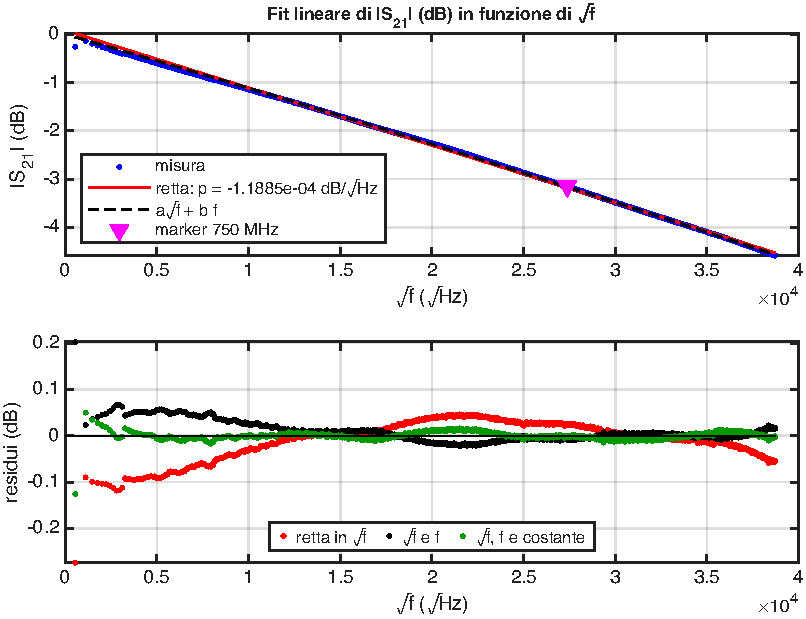
\includegraphics[width=0.8\textwidth]{Images/Relazione1_Foto/p3_fit_sqrtf.pdf}
    \caption{In alto: $|S_{21}|$ in funzione di $\sqrt f$ (punti blu) con la retta di regressione (rosso), il modello $a\sqrt f + bf$ (nero) e il marker del punto~2. In basso: residui della retta e dei due modelli con il termine del dielettrico.}
    \label{fig:p3}
\end{figure}

\section{Costante \texorpdfstring{$\alpha'$}{alpha'} e attenuazione a \texorpdfstring{750\,MHz}{750 MHz}}
Dalla pendenza, con $L = 10$\,m e $20\log_{10}\mathrm{e} = 8.6859$:
\begin{equation}
\alpha' = \frac{1.18847\cdot10^{-4}}{8.6859\cdot\sqrt{2\pi}\cdot10} = (5.4586\pm0.0040)\cdot10^{-7}\ \mathrm{m}^{-1}(\mathrm{rad/s})^{-1/2},
\end{equation}
con incertezza relativa dello 0.07\,\%; il valore è dello stesso ordine di grandezza di quello dell'esempio visto a lezione ($5\cdot10^{-7}$). L'attenuazione a 750\,MHz prevista con $\alpha'$:
\begin{equation}
A_{fit}(750\ \mathrm{MHz}) = -p\sqrt f = 1.18847\cdot10^{-4}\cdot27\,386 = (3.2547\pm0.0024)\ \mathrm{dB},
\end{equation}
con $u(A_{fit}) = \sqrt f\,u(p)$.

\section{Confronto con il marker}
$A_{fit}$ supera il valore del marker, $(3.153\pm0.026)$\,dB, di 0.102\,dB, cioè di 3.9 volte l'incertezza combinata $\sqrt{0.0024^2+0.026^2} = 0.026$\,dB: \textbf{i due valori non sono compatibili}. La causa è il modello, non la misura:
\begin{itemize}
  \item i residui della retta (fig.~\ref{fig:p3}, in basso) non sono rumore ma un arco sistematico, da $-0.12$ a $+0.05$\,dB (escluso il primo punto, a 300\,kHz), molto più grande del rumore della traccia (0.001\,dB);
  \item l'intercetta $q = 0.077$\,dB è diversa da zero di più di 30 volte la sua incertezza, mentre il modello prevede una retta per l'origine: un cavo passivo non può avere $|S_{21}|>0$\,dB, e il fit compensa con l'intercetta una curvatura che il modello non contiene.
\end{itemize}
La retta completa, con l'intercetta, dà invece a 750\,MHz un'attenuazione di 3.178\,dB, a 0.025\,dB dal marker, cioè entro la sua incertezza: le misure dei punti 2 e 3 sono coerenti, è il modello per l'origine con la sola $\alpha'$ a non bastare. Aggiungendo il termine del dielettrico, proporzionale a $f$, lo scarto quadratico medio dei residui scende da 0.0313 a 0.0155\,dB e l'attenuazione a 750\,MHz diventa 3.161\,dB; con anche un piccolo termine costante (connettori, residuo della calibrazione), $A = a\sqrt f + bf + c$, scende a 0.0076\,dB e $A(750\ \mathrm{MHz}) = 3.1525$\,dB, in accordo con il marker. A 750\,MHz questo modello ripartisce l'attenuazione in 2.81\,dB dovuti ai conduttori, 0.26\,dB al dielettrico e 0.08\,dB costanti.

In conclusione: il modello della practice segue bene l'andamento della misura ($r = -0.99958$), ma, attribuendo tutta la perdita alla legge in $\sqrt f$, a 750\,MHz sovrastima l'attenuazione di 0.10\,dB, cioè di circa il 3\,\%. Il valore misurato dell'attenuazione è quello del marker, $(3.153\pm0.026)$\,dB; $\alpha' = (5.4586\pm0.0040)\cdot10^{-7}$\,m$^{-1}$(rad/s)$^{-1/2}$ è il parametro della legge in $\sqrt f$ che meglio approssima la misura su tutta la banda, e la sua incertezza (solo statistica) non comprende l'errore del modello.

% =====================================================================
% Capitolo 4
% =====================================================================
\chapter{Misura della fase di \texorpdfstring{$S_{21}$}{S21} tramite delay elettrico}
Lo scopo della seguente misura è valutare l'electrical delay in funzione del parametro S21, che, essendo un numero complesso, può essere espresso nella seguente forma:
\begin{equation}
S21 = |S21|exp(-j\omega\tau)
\end{equation}
\section{Fase di \texorpdfstring{$S_{21}$}{S21} e compensazione del ritardo}
Andando a visualizzare la fase sul VNA, individueremo un segnale periodico tra -180\(°\) e +180\(°\) come si può osservare in figura \ref{fig:4_1}.
\begin{figure}[H]
    \centering
    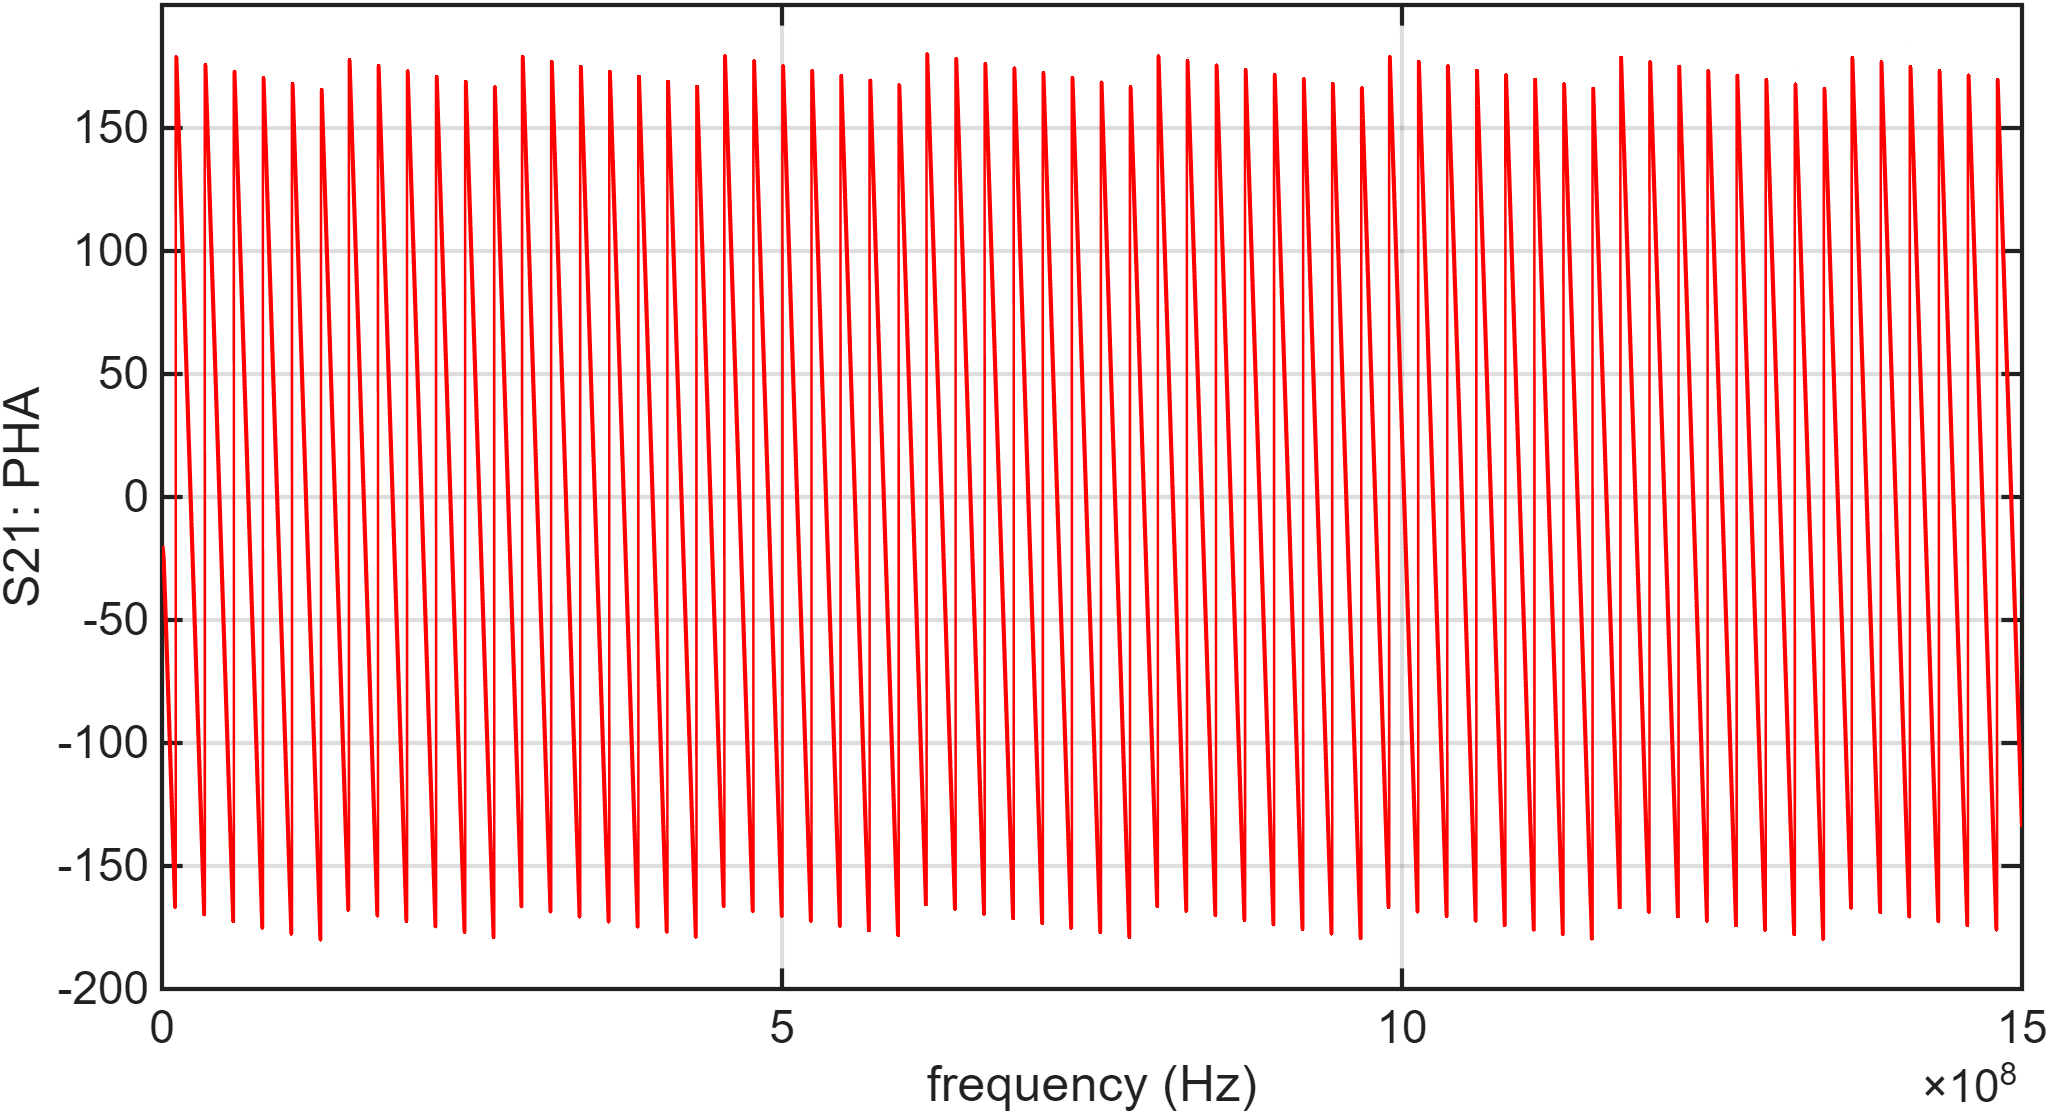
\includegraphics[width=0.6\textwidth]{./Images/Relazione1_Foto/4_1_fase_wrapped_cavo_10m.png} 
    \caption{Fase S21 wrapped}
    \label{fig:4_1}
\end{figure}
Questo andamento periodico è causato dal metodo di visualizzazione adottato dal VNA ed è costituito dalla visualizzazione del valore principale dell'argomento che riporta la fase nel suo intervallo convenzionale [-180,+180], dunque nel momento in cui il valore della fase oltrepassa l'intervallo di visualizzazione del VNA, quest'ultimo la riporta nel range e ciò ne determina il salto e la periodicità della fase.
Come visto nella formula \ref{fig:4_1} la fase di $S_{21}$ decresce linearmente all'aumentare della frequenza e al fine di ricavare l'electrical delay dovuto al cavo coassiale (dopo aver srotolato la fase, ottenendo la fase unwrapped mostrata in figura \ref{fig:4_2}) siamo andati ad aggiungere un ritardo fittizio in modo tale da annullare la pendenza della fase unwrapped di $S_{21}$. 
\begin{equation}
\Phi(S21) = -\omega\tau+\omega\tau' = 0
\end{equation}
con \(\tau'\)=42.88ns, ritardo fittizio che abbiamo aggiunto tramite il VNA.
\begin{figure}[H]
    \centering
    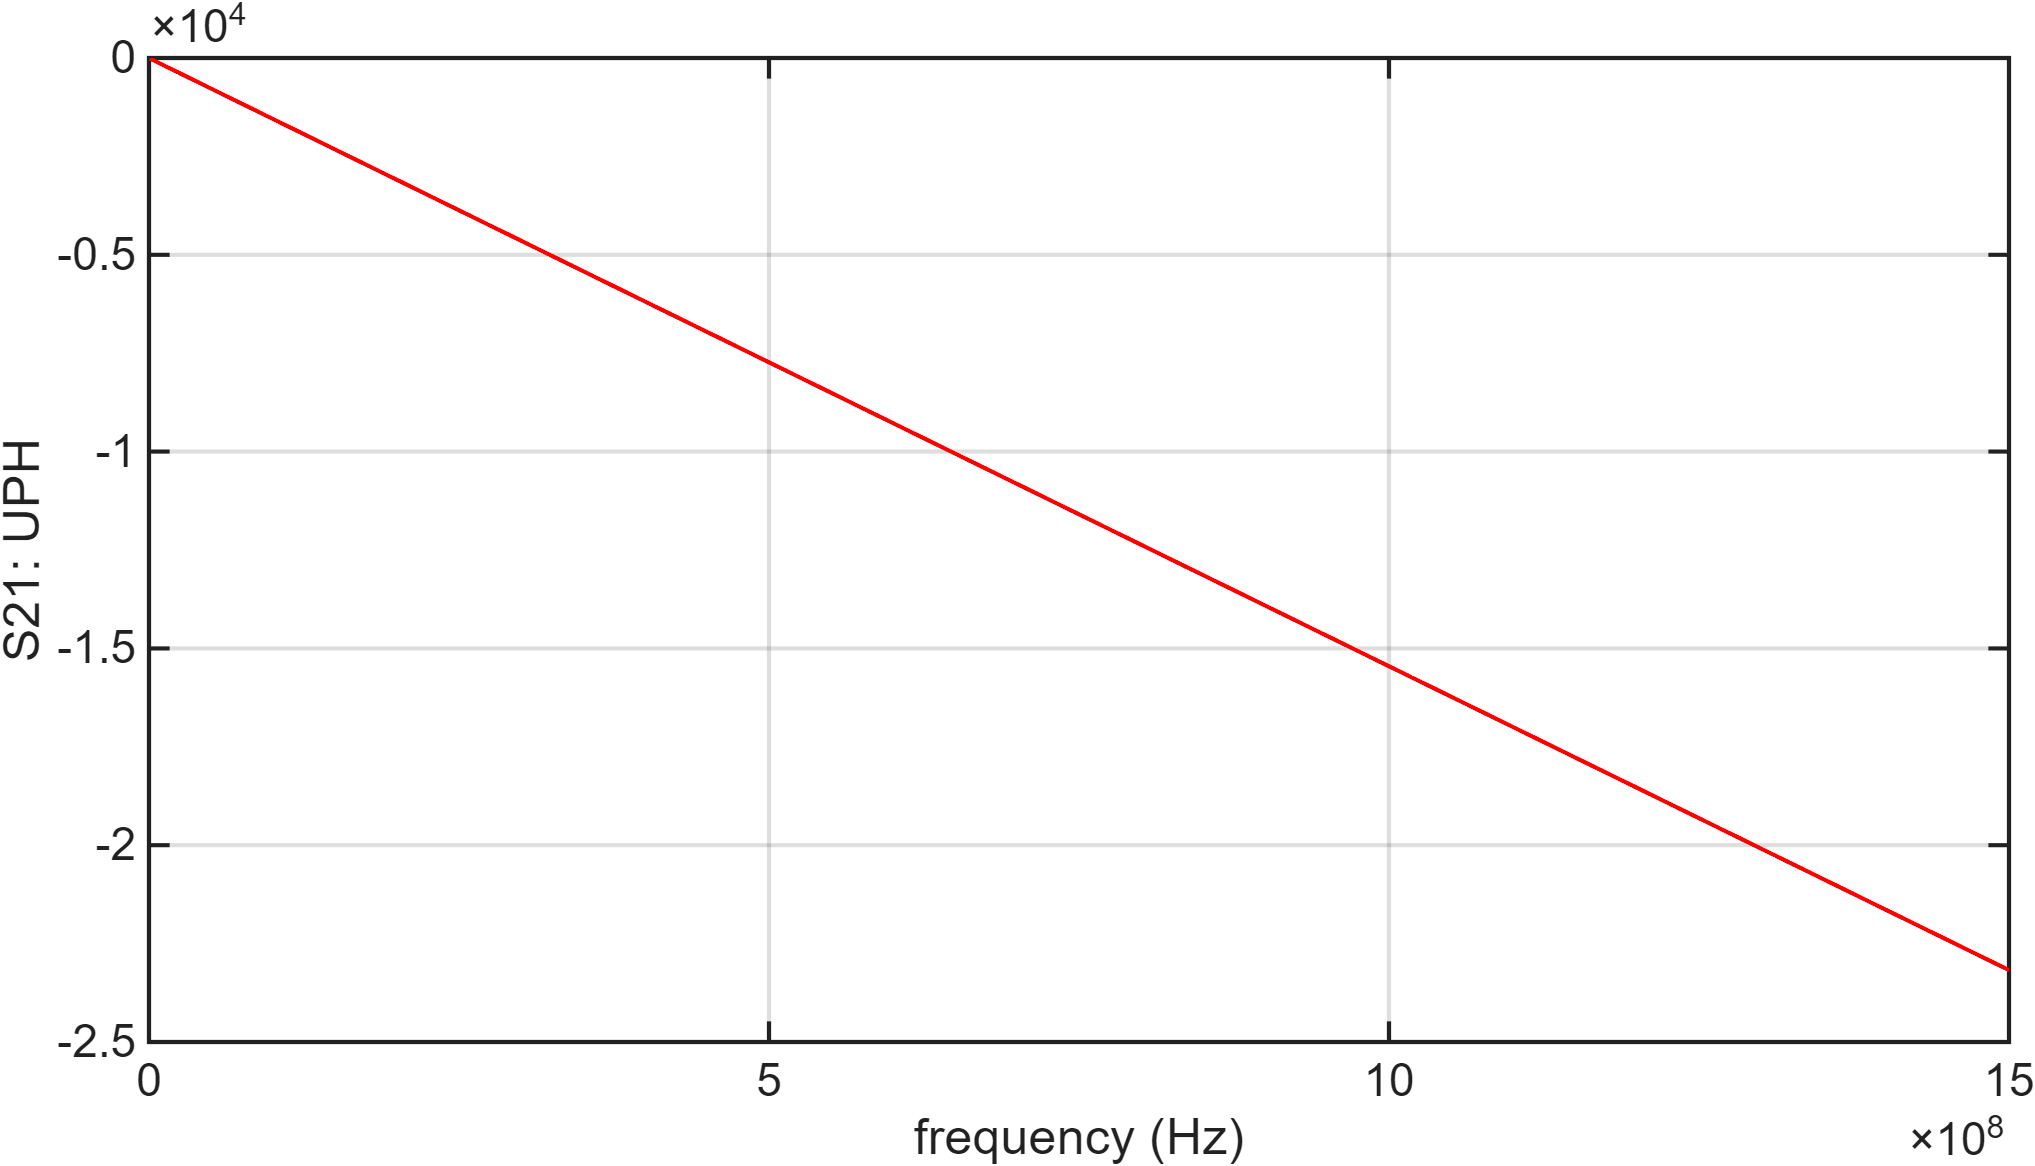
\includegraphics[width=0.6\textwidth]{./Images/Relazione1_Foto/4_2_boh_fase_cavo_10m_unwrap.png} 
    \caption{Fase S21 unwrapped}
    \label{fig:4_2}
\end{figure}
\section{Costante dielettrica e indice di rifrazione}
Dalla teoria, sappiamo che questo tipo di misura ci permette di stimare la costante dielettrica \(\epsilon_r\) e l'indice di rifrazione del cavo sotto test, tramite le seguenti formule:
\begin{equation}
L0 = c\tau'
\end{equation}
\begin{equation}
n = \sqrt{\epsilon_r} = L0/L
\end{equation}
Essendo \(L = 10 m\) la lunghezza del cavo e \(c\) la velocità della luce nel vuoto, otteniamo i seguenti valori misurati:
\begin{equation}
\epsilon_r = 1,6548
\end{equation}
\begin{equation}
n = 1,2864
\end{equation}
\section{Limite dello strumento}
\begin{figure}[H]
    \centering
    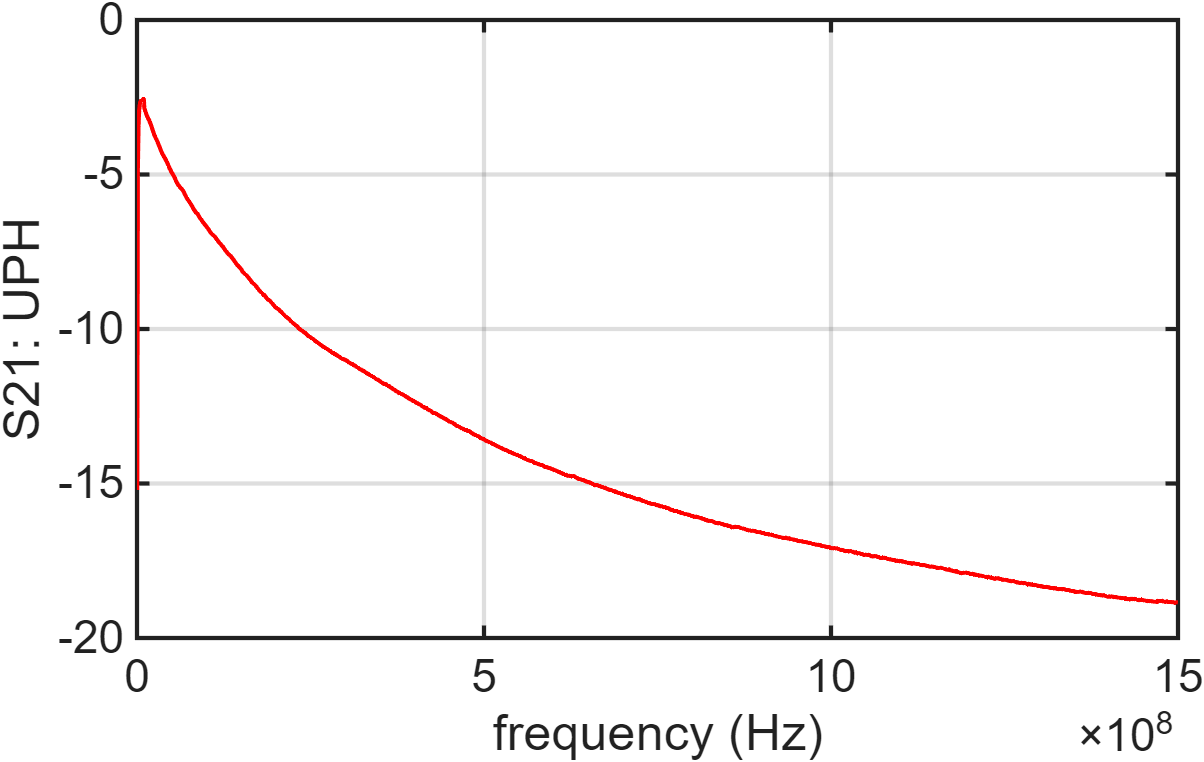
\includegraphics[width=0.6\textwidth]{./Images/Relazione1_Foto/4_3_1_RITARDO_DI_FASE_SCALA_PICCOLA_RIMANE_PARTE_NON_LINEARE.png} 
    \caption{Zoom sulla fase S21 wrapped}
    \label{fig:4_3}
\end{figure}
Nella figura \ref{fig:4_3} osserviamo come, facendo uno zoom sulla pendenza della curva fase S21 in funzione della frequenza, questa non sia stata completamente appiattita; questo effetto ci mostra il limite effettivo dello strumento.

% =====================================================================
% Capitolo 5
% =====================================================================
\chapter{Misura della fase di \texorpdfstring{$S_{21}$}{S21} tramite "phase slope"}
L'obiettivo di questa misura è determinare dalla misura di fase (riportata unwrapped in figura \ref{fig:5_1}) il ritardo elettrico del cavo coassiale tramite la pendenza della fase di $S_{21}$.
\begin{equation}
\tau = \frac{-p(rad)}{2\pi}
\end{equation}
\begin{figure}[H]
    \centering
    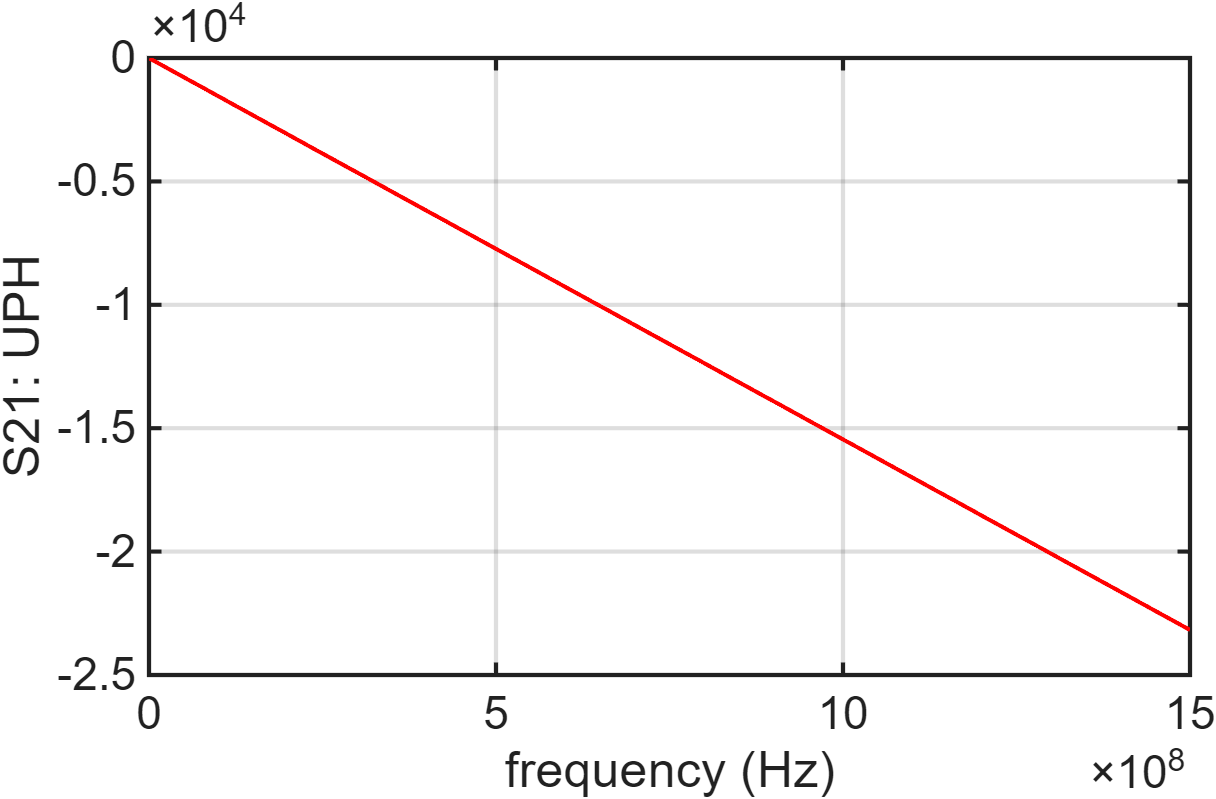
\includegraphics[width=0.6\textwidth]{./Images/Relazione1_Foto/5_1_fase_di_s21_e_basta.png} 
    \caption{Misura di fase unwrapped S21}
    \label{fig:5_1}
\end{figure}
\section{Regressione lineare della fase}
Utilizzando la routine MATLAB LinearFit.m (figura \ref{fig:5_2}) otteniamo il valore della pendenza e la sua incertezza, con unità di misura gradi su hertz.
\begin{figure}[H]
    \centering
    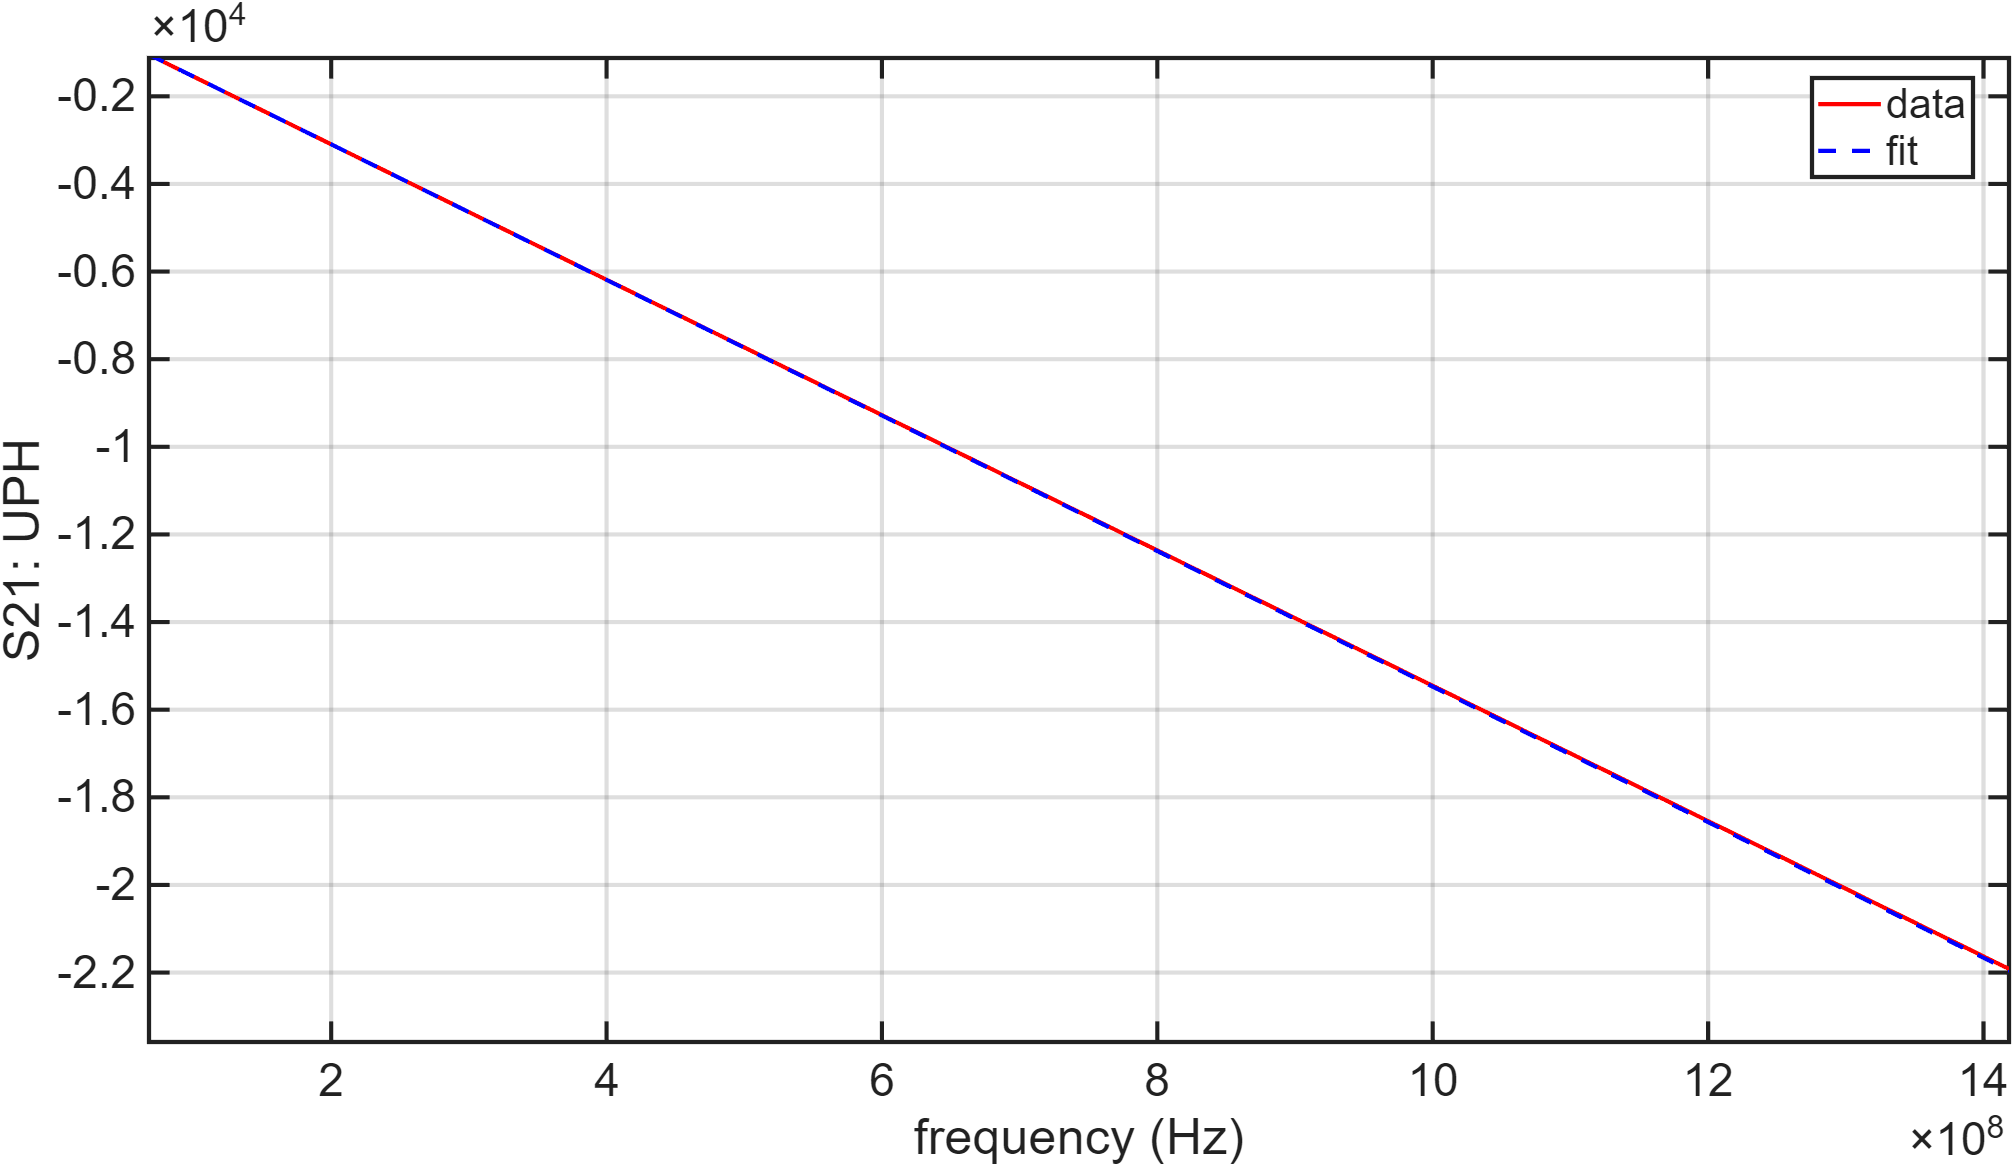
\includegraphics[width=0.6\textwidth]{./Images/Relazione1_Foto/5_2_fase_con_linear_fit.png} 
    \caption{Misura di fase con fit lineare}
    \label{fig:5_2}
\end{figure}

\begin{equation}
p_m = -1,5472\cdot 10^{-5} \quad °/Hz
\end{equation}
\begin{equation}
\sigma_p = 4,6777775720636 \cdot 10^{-9} \quad °/Hz
\end{equation}

\begin{equation}
  p= (-1,5472 \pm 0.0005 )\cdot10^{-5} \quad °/Hz
\end{equation}

\section{Ritardo elettrico}
Ora passiamo a calcolare il ritardo elettrico, ricordando che la pendenza è espressa in gradi:
\begin{equation}
  \tau_m=42,978\ ns
\end{equation}
\begin{equation}
  \sigma_{\tau}=\frac{\sigma_{p}}{360}= 0,013\ ns
\end{equation}
\begin{equation}
  \tau= [42,978 \pm 0,013]\ ns 
\end{equation}
\section{Confronto con il delay elettrico}
Infine andiamo a confrontare le misure del ritardo elettrico del cavo coassiale eseguite al punto 4 e al punto 5 della relazione.

I due valori (42,88 ns e 42,978 ns) differiscono di circa un decimo di nanosecondo, cioè di circa lo 0,2\%. Questa differenza è circa 7,5 volte l'incertezza del fit, che però è solo statistica; inoltre il valore del punto 4 è ottenuto regolando il ritardo fino ad annullare la pendenza della fase e non ha un'incertezza associata. Le due misure sono quindi in buon accordo, ma non possiamo affermare che siano compatibili entro l'incertezza.

% =====================================================================
% Capitolo 6
% =====================================================================
\chapter{Misura di riflessione del cavo}

Il setup sperimentale di questa misura è stato fatto collegando il cavo coassiale alla porta 1 del VNA e lasciandone l'altra estremità aperta.

\section{Ritardo dalle oscillazioni di \texorpdfstring{$|S_{11}|$}{|S11|}}
La figura \ref{fig:6_1} grafica l'andamento del modulo di $S_{11}$ in dB. Da questo setup possiamo misurare l'electrical delay, attraverso l'utilizzo delle seguenti formule:
\begin{equation}
\Delta f = \frac{f_2-f_1}{N} = 0.0115 GHz
\end{equation}
dove $f_2$ e $f_1$ sono i valori di frequenza presi dallo zoom della figura \ref{fig:6_2}, ed $N$ è il numero di oscillazioni periodiche tra i due marker.
\begin{figure}[H]
    \centering
    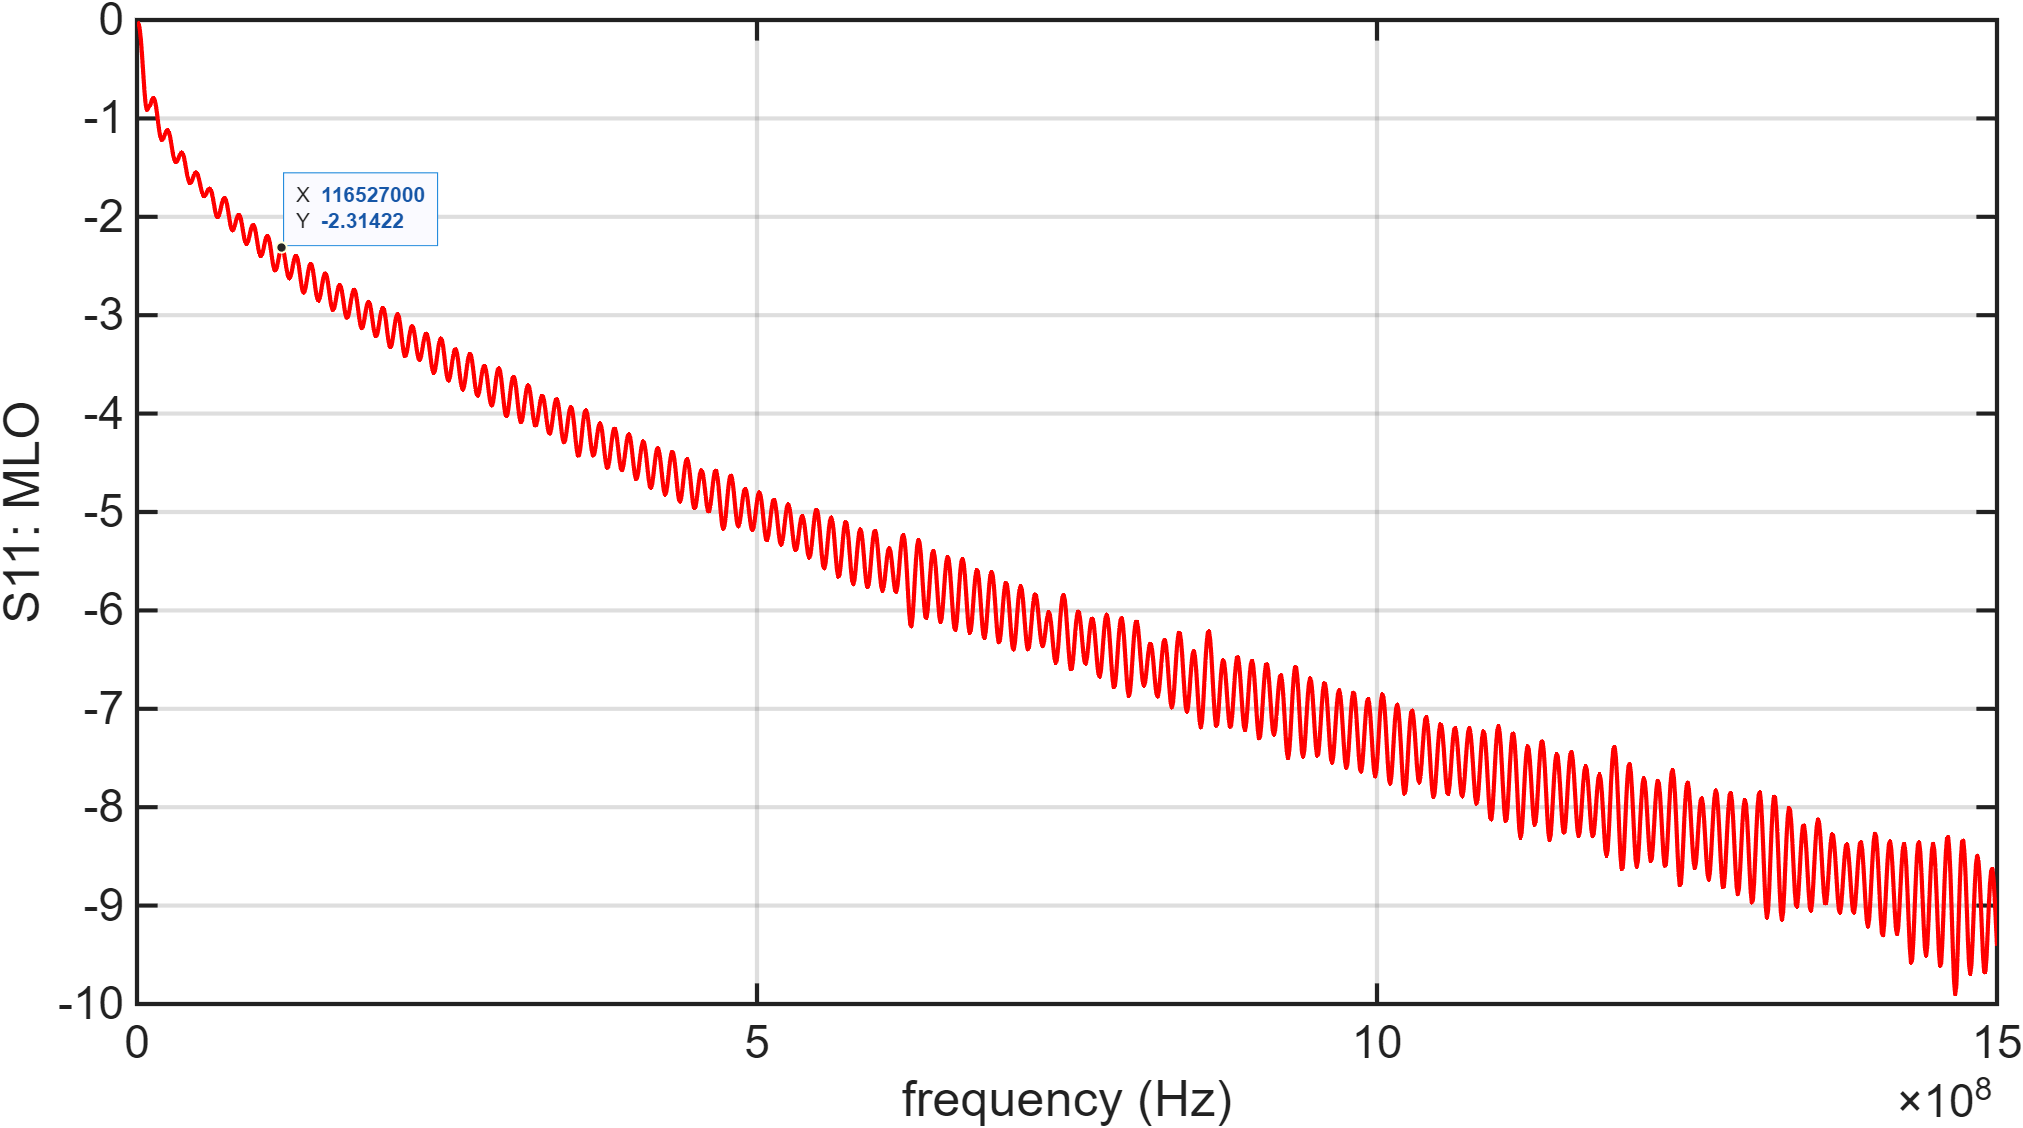
\includegraphics[width=0.6\textwidth]{./Images/Relazione1_Foto/6_1_modulo_dB_S11_porta2_aperta.png} 
    \caption{Modulo S11 open end}
    \label{fig:6_1}
\end{figure}
\begin{figure}[H]
    \centering
    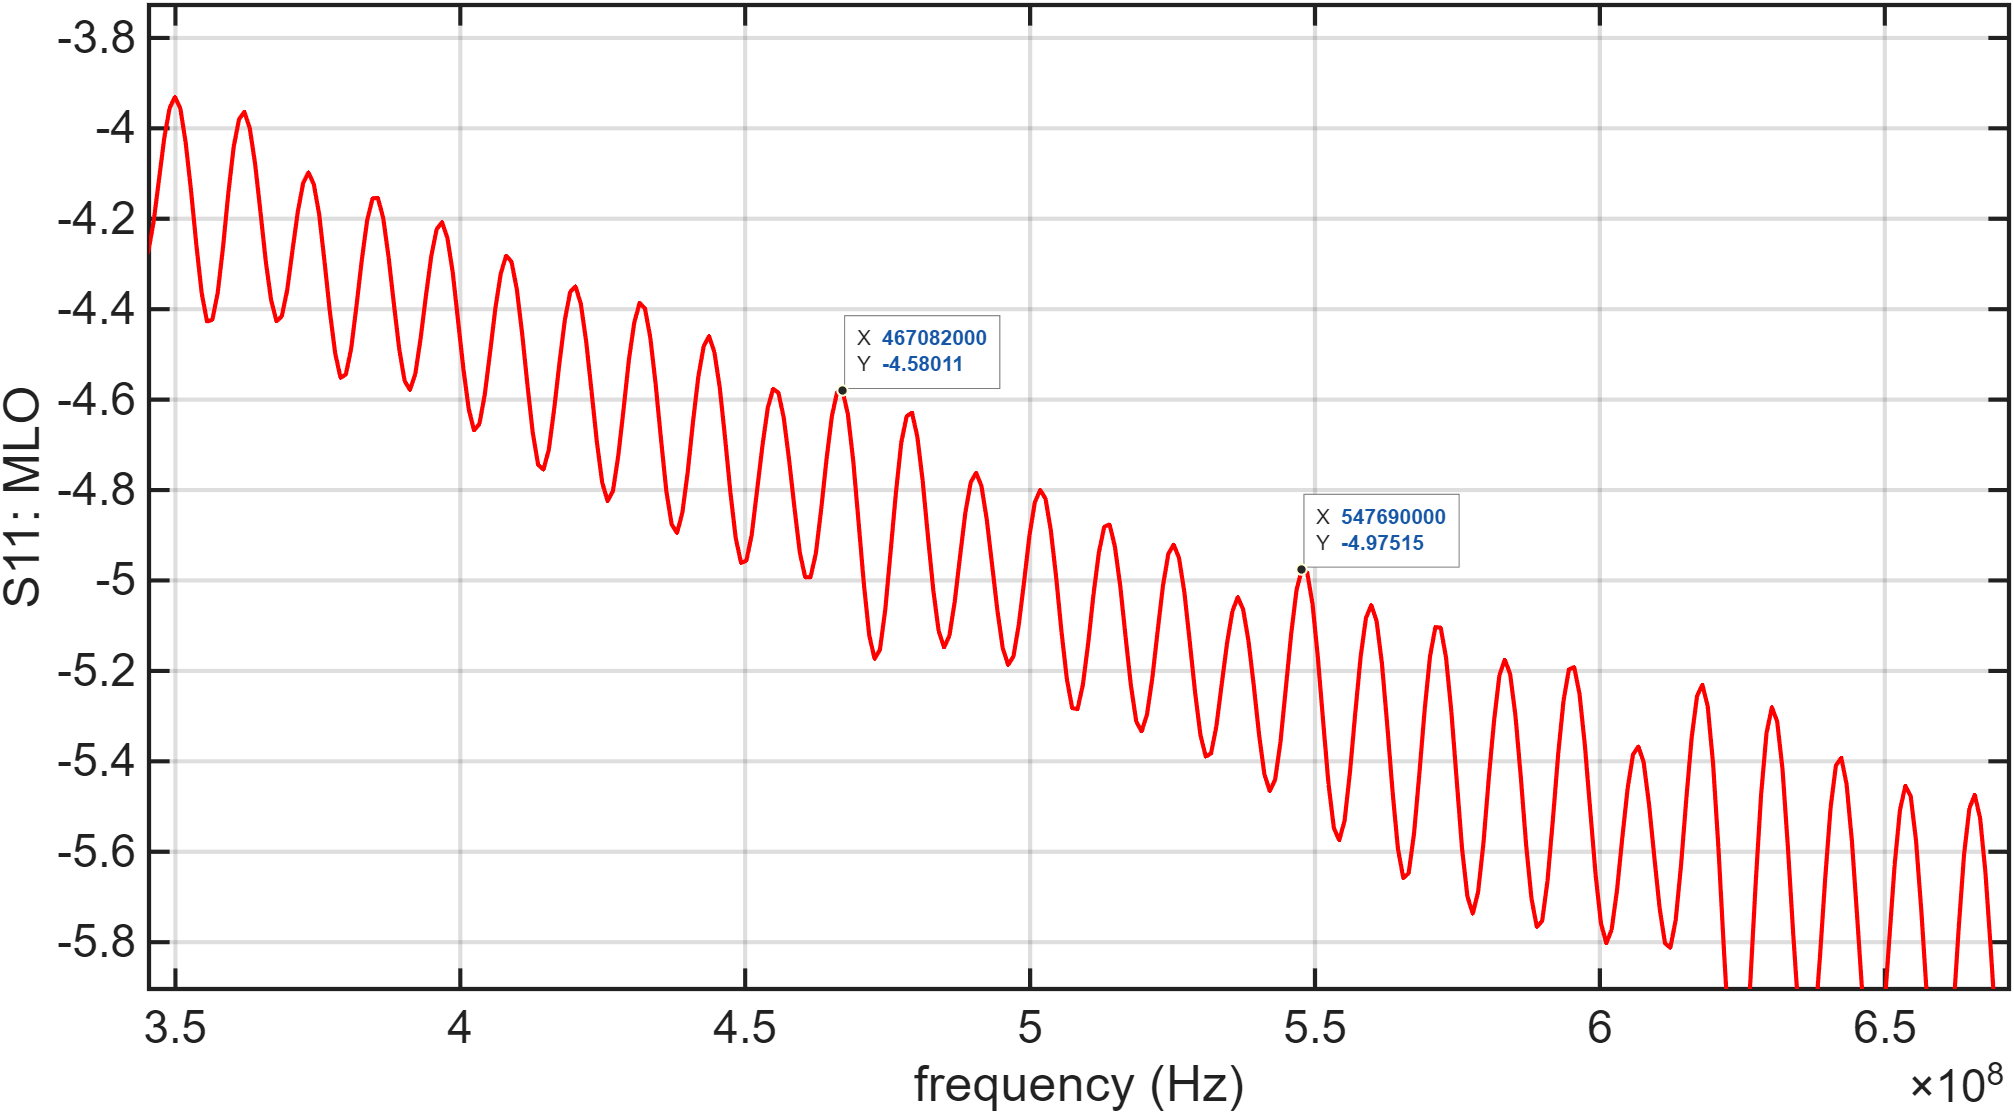
\includegraphics[width=0.6\textwidth]{./Images/Relazione1_Foto/6_2_extra.png} 
    \caption{Zoom modulo S11 open end}
    \label{fig:6_2_extra}
\end{figure}
L'electrical delay può essere calcolato mediante:
\begin{equation}
\tau = \frac{1}{2\Delta f}\ = 43,42 ns
\end{equation}
Successivamente possiamo ricavare l'indice di rifrazione $n$:
\begin{equation}
n = \frac{c}{2L\Delta f} = 1.303,
\end{equation}
il quale non si discosta molto dal valore ricavato al punto 4, ovvero: \( n = 1,2864\).

\section{Ritardo dalla pendenza della fase di \texorpdfstring{$S_{11}$}{S11}}
\begin{figure}[H]
    \centering
    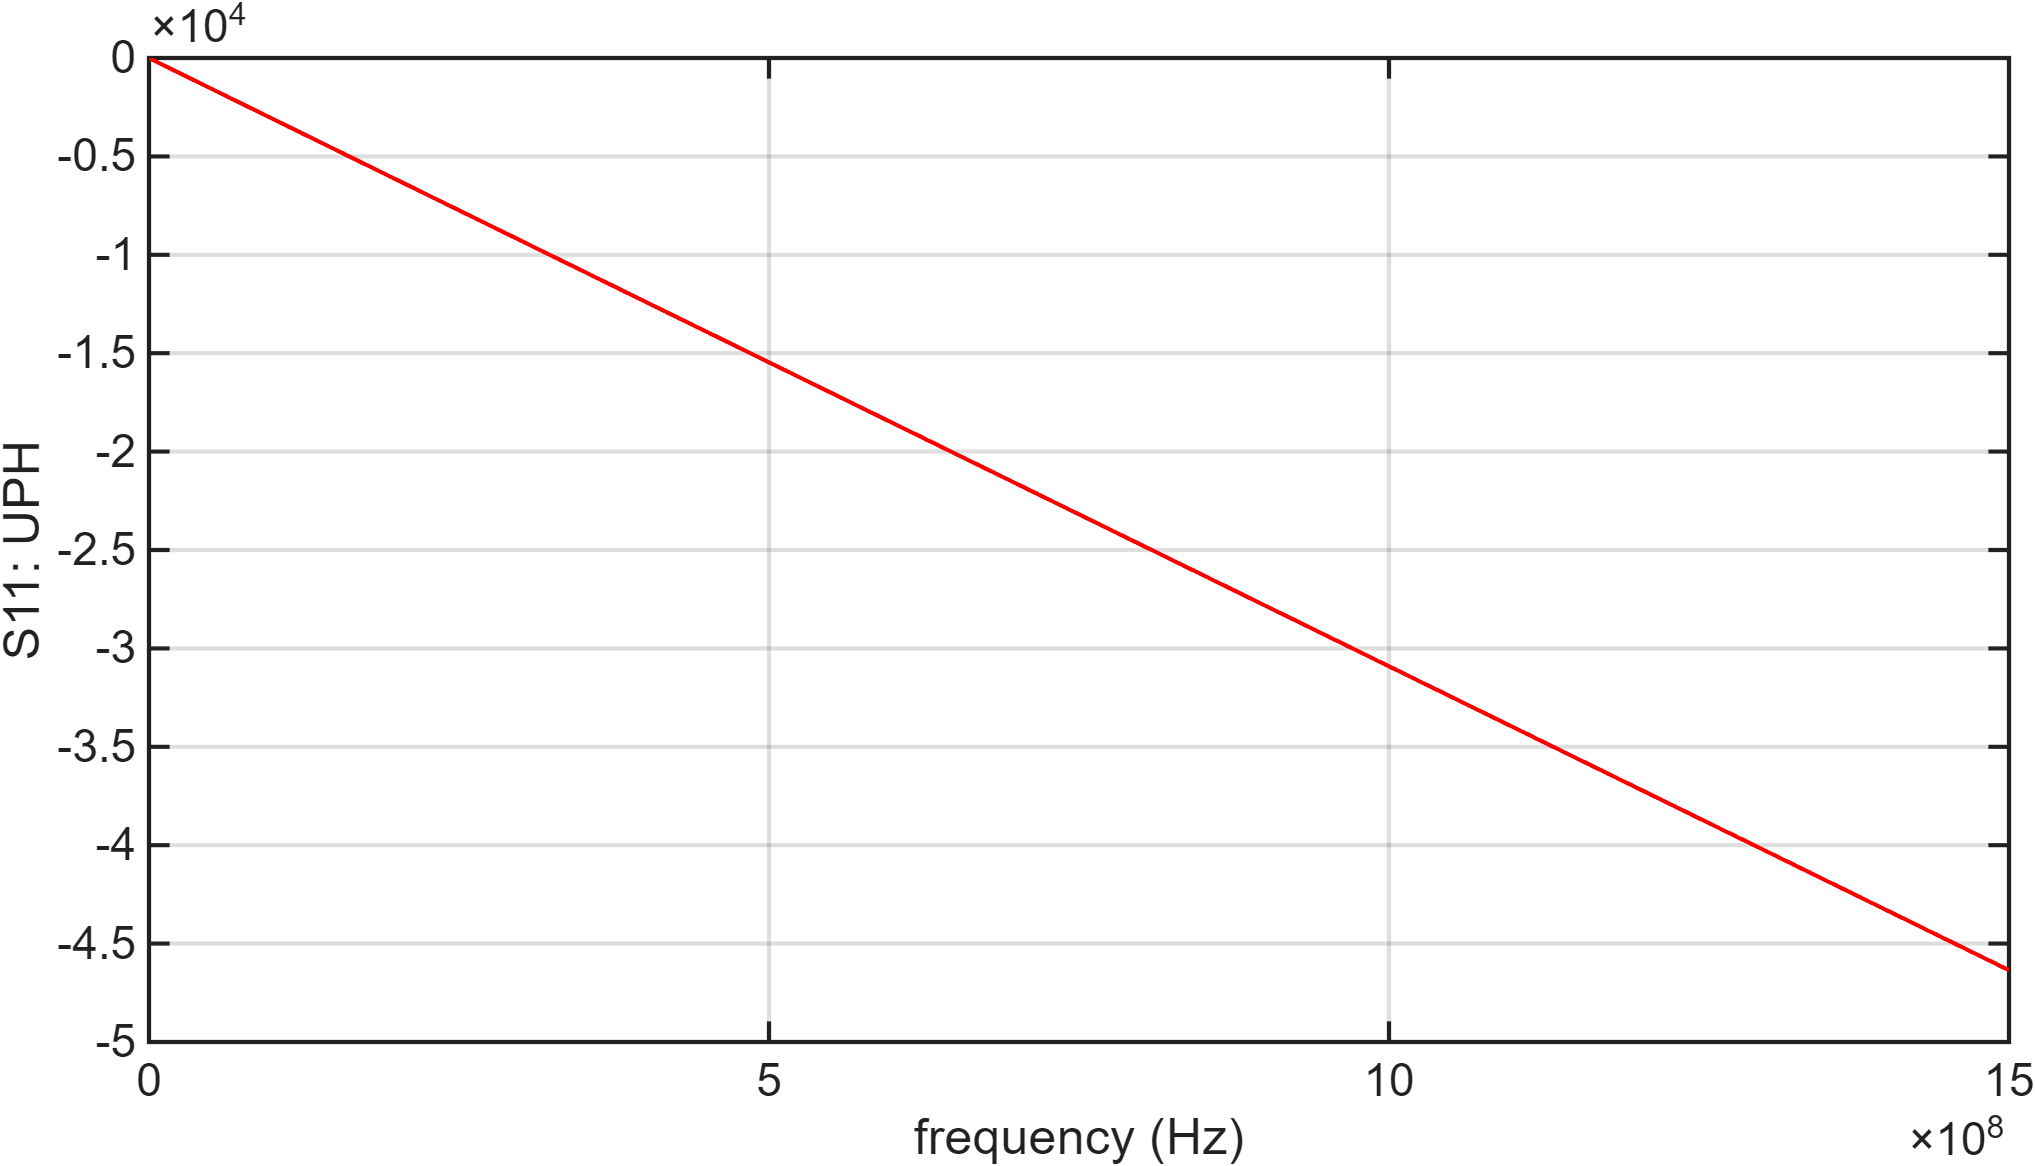
\includegraphics[width=0.6\textwidth]{./Images/Relazione1_Foto/6_2_Fase_S11_unwrapped_porta_2_in_aperto.png} 
    \caption{}
    \label{fig:6_2}
\end{figure}
\begin{figure}[H]
    \centering
    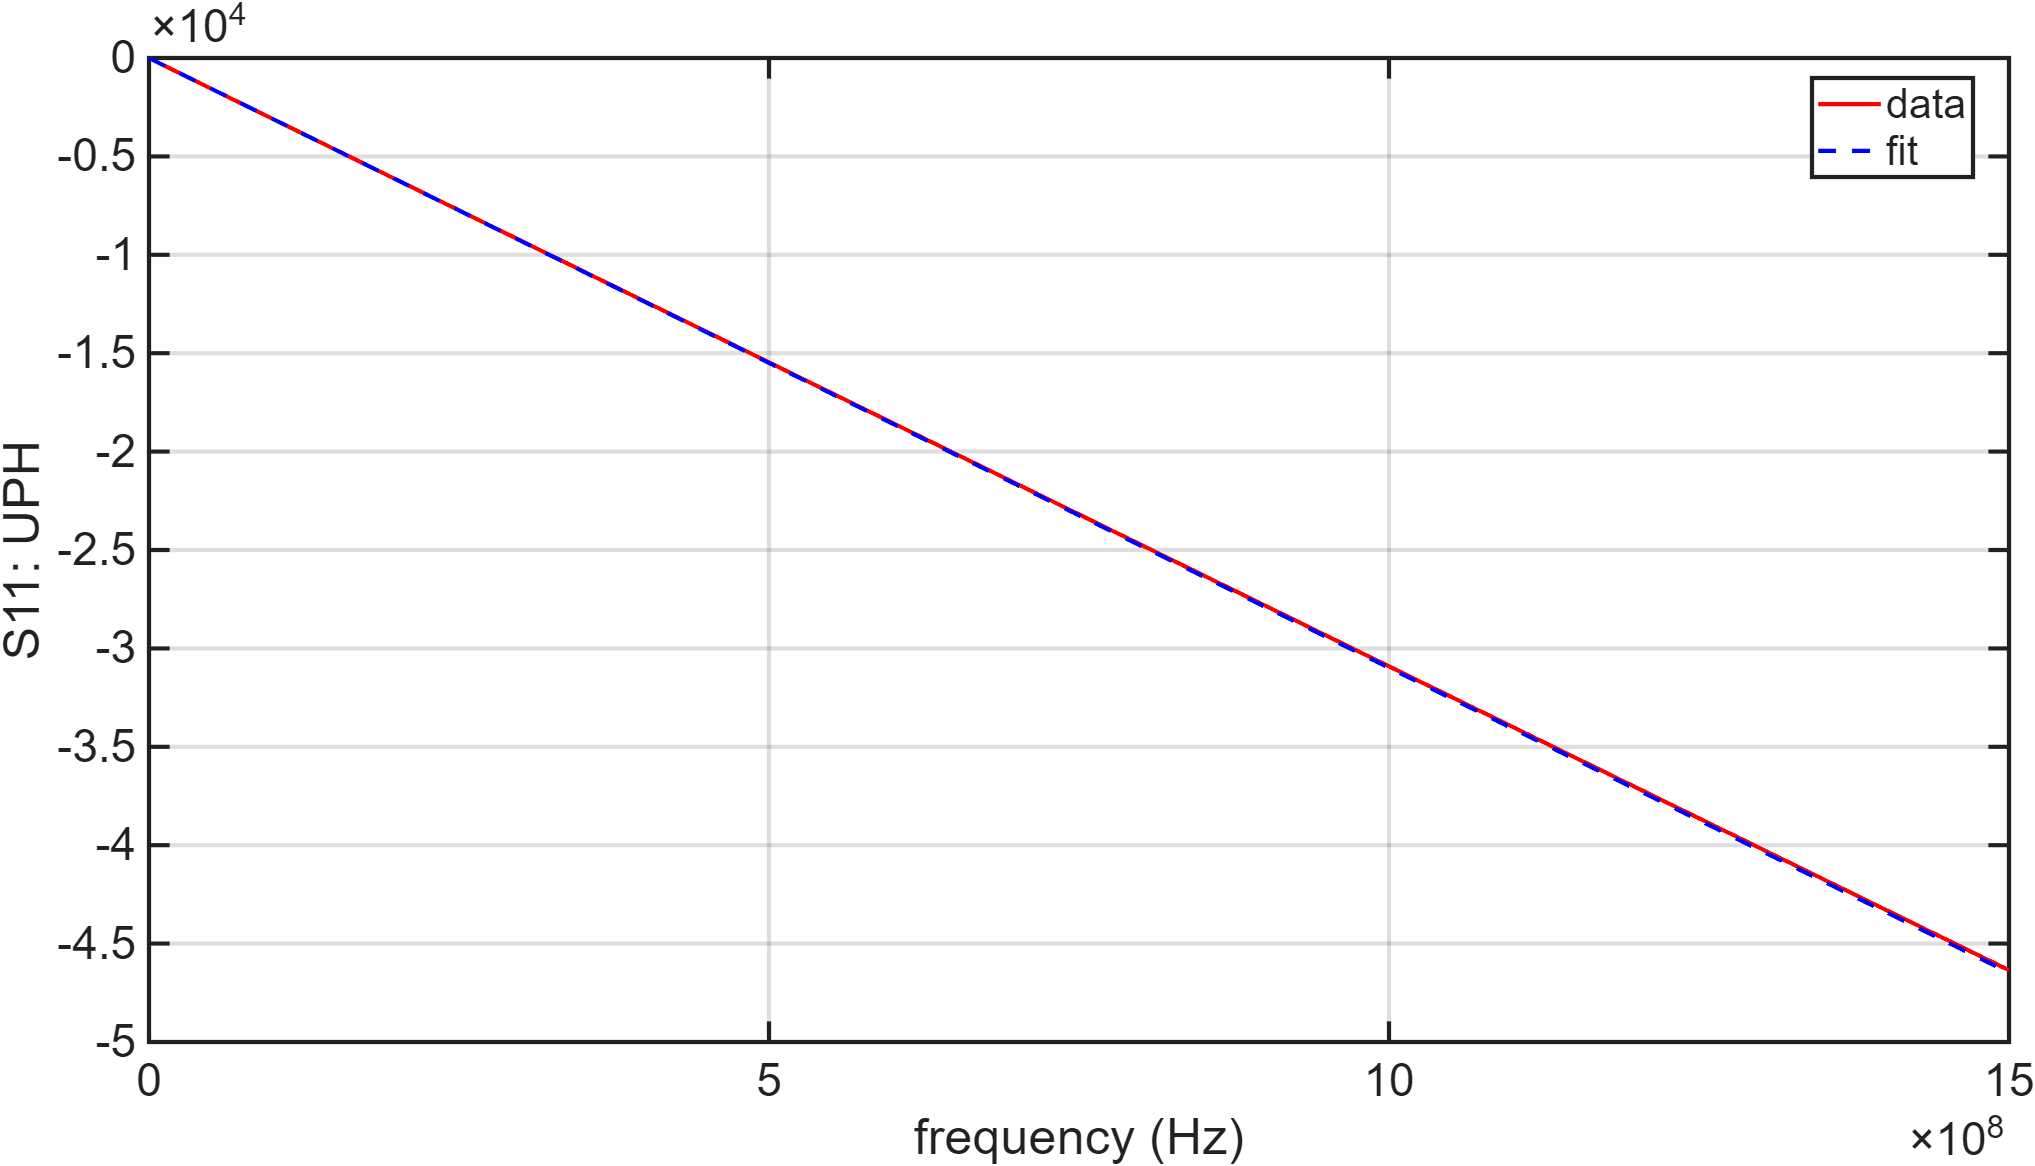
\includegraphics[width=0.6\textwidth]{./Images/Relazione1_Foto/6_2_1_Fase_S11_unwrapped_porta_2_in_aperto_linear_fit.png} 
    \caption{}
    \label{fig:6_2_1}
\end{figure}

\section{Confronto fra i quattro metodi}
\begin{center}
\begin{tabular}{|c|c|c|c|c|}
\hline
Metodo & \shortstack{Electrical delay\\(punto 4)} & \shortstack{Pendenza fase $S_{21}$\\(punto 5)} & \shortstack{Oscillazioni $|S_{11}|$\\(punto 6)} & \shortstack{Pendenza fase $S_{11}$\\(punto 6)} \\ \hline
$\tau$ [ns] & 42,88 & 42,98 & 43,42 & 43,03 \\ \hline
\end{tabular}
\end{center}
I quattro metodi danno valori molto vicini: la differenza massima è di 0,54 ns, cioè circa l'1,3\%. Il valore più lontano è quello ricavato dalle oscillazioni di $|S_{11}|$, che dipende dai minimi scelti per calcolare $\Delta f$; gli altri tre differiscono al massimo di 0,15 ns.

% =====================================================================
% Capitolo 7
% =====================================================================
\chapter{Misura di impedenza e permettività di una microstriscia}
\section{Misura dell'impedenza caratteristica}
Per la misurazione avevamo due microstrisce, che distingueremo in seguito come "microstriscia larga" e "microstriscia stretta" in base 
alla larghezza del metallo della microstriscia. Per
entrambe le microstrisce abbiamo usato la tecnica di trasformazione a "$\lambda/4$" e la tecnica di misura "corto circuito-
circuito aperto". Le misurazioni sono state fatte tra 2MHz e 200MHz, con calibrazione dello strumento in queste frequenze, tranne quelle in circuito aperto e in corto circuito della microstriscia larga, fatte tra 1MHz e 100MHz.

\subsection{Microstriscia larga}
Per prima abbiamo valutato la microstriscia larga. Graficata l'impedenza misurata, ci siamo spostati con il marker fino al punto 
in cui la parte immaginaria è nulla (non esattamente nulla, ma il valore più piccolo riscontrato). In questo punto l'impedenza vale:
\begin{equation}
Z_{IN}=12.37 +j0.2 \quad \Omega
\end{equation}

\begin{figure}[H]
\centering
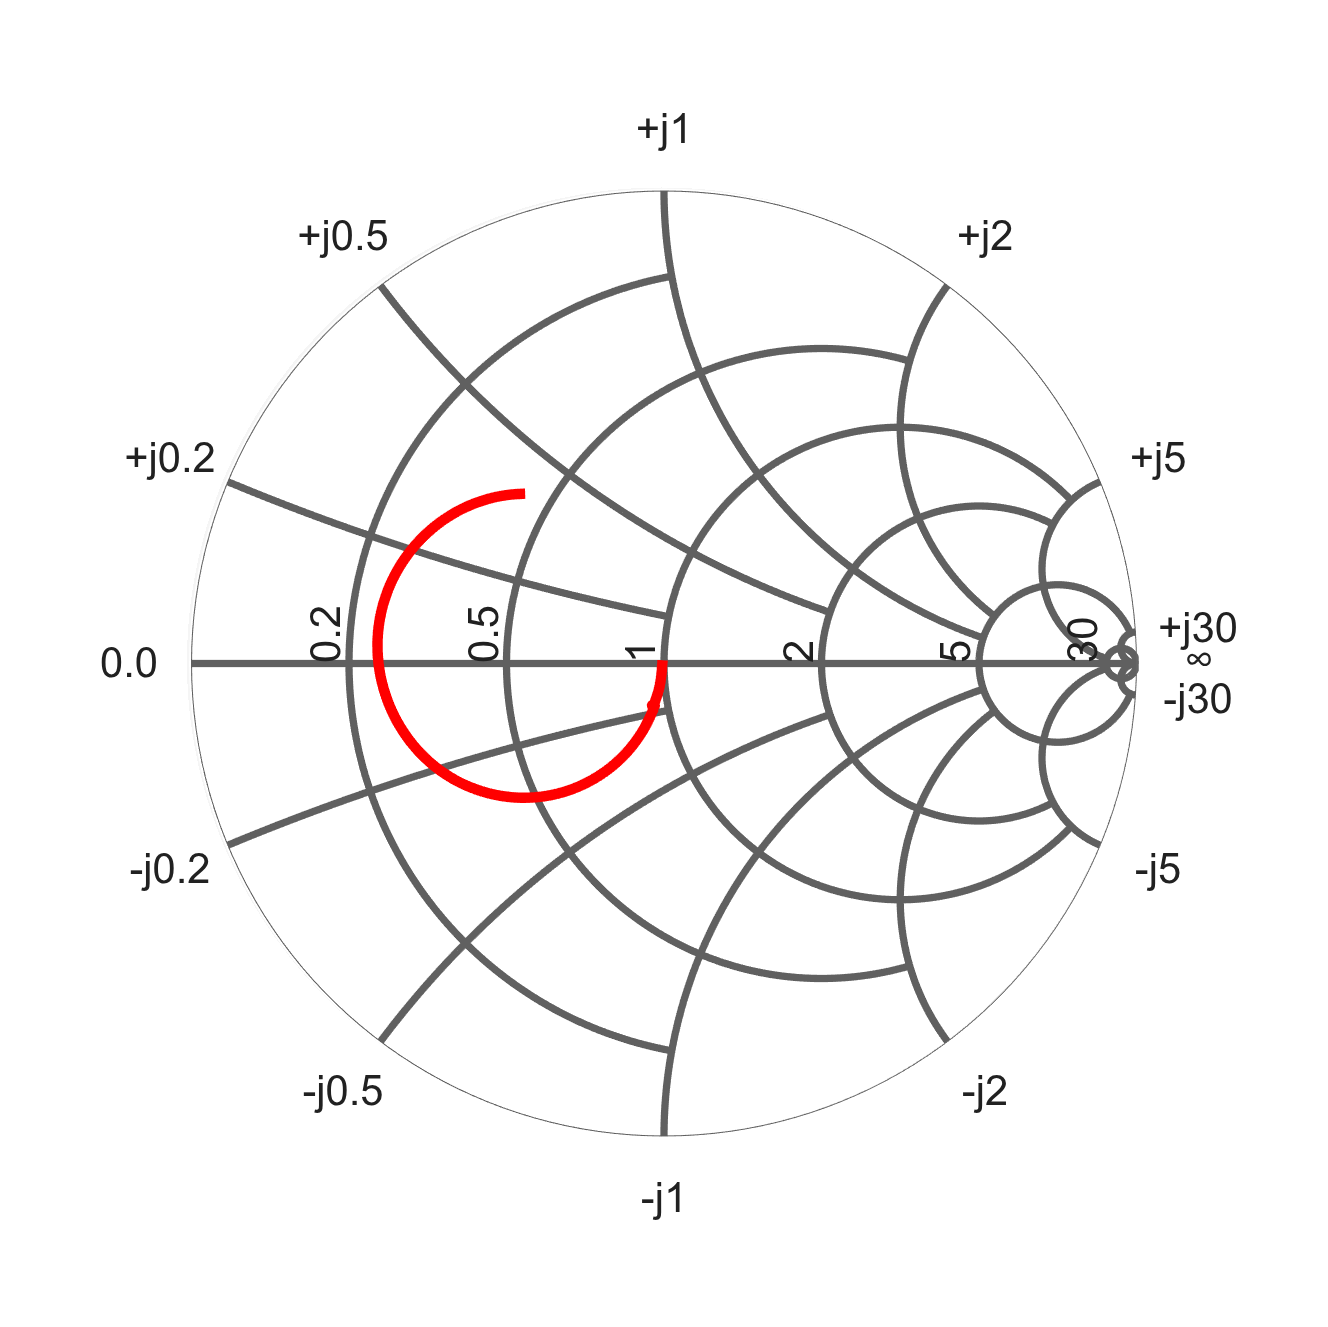
\includegraphics[width=0.4\textwidth]{./Images/Relazione1_Foto/7_1_microstrip_larga_lambda_quarti.png}
\caption{Smith chart dell'impedenza tramite tecnica "$\lambda/4$".}
\end{figure}

Da ciò l'impedenza caratteristica è:
\begin{equation}
Z_C=\sqrt{Z_{IN}\cdot Z_0}=\sqrt{12.37\cdot50}\simeq 24.87 \quad \Omega
\end{equation}
Siamo passati poi a valutare la stessa impedenza tramite il secondo metodo. In questo caso sono necessarie due misurazioni, 
una con chiusura in circuito aperto (impedenza indicata con $Z_{OC}$) e una con chiusura in corto (impedenza indicata con $Z_{SC}$).
 Siamo partiti con la misura in circuito aperto, e ci siamo tenuti a basse frequenze per tenere l'impedenza il più possibile immaginaria.
A 50MHz abbiamo misurato: 
\begin{equation}
Z_{OC}=0.845-j32 \quad \Omega
\end{equation}
\begin{figure}[H]
  \centering
  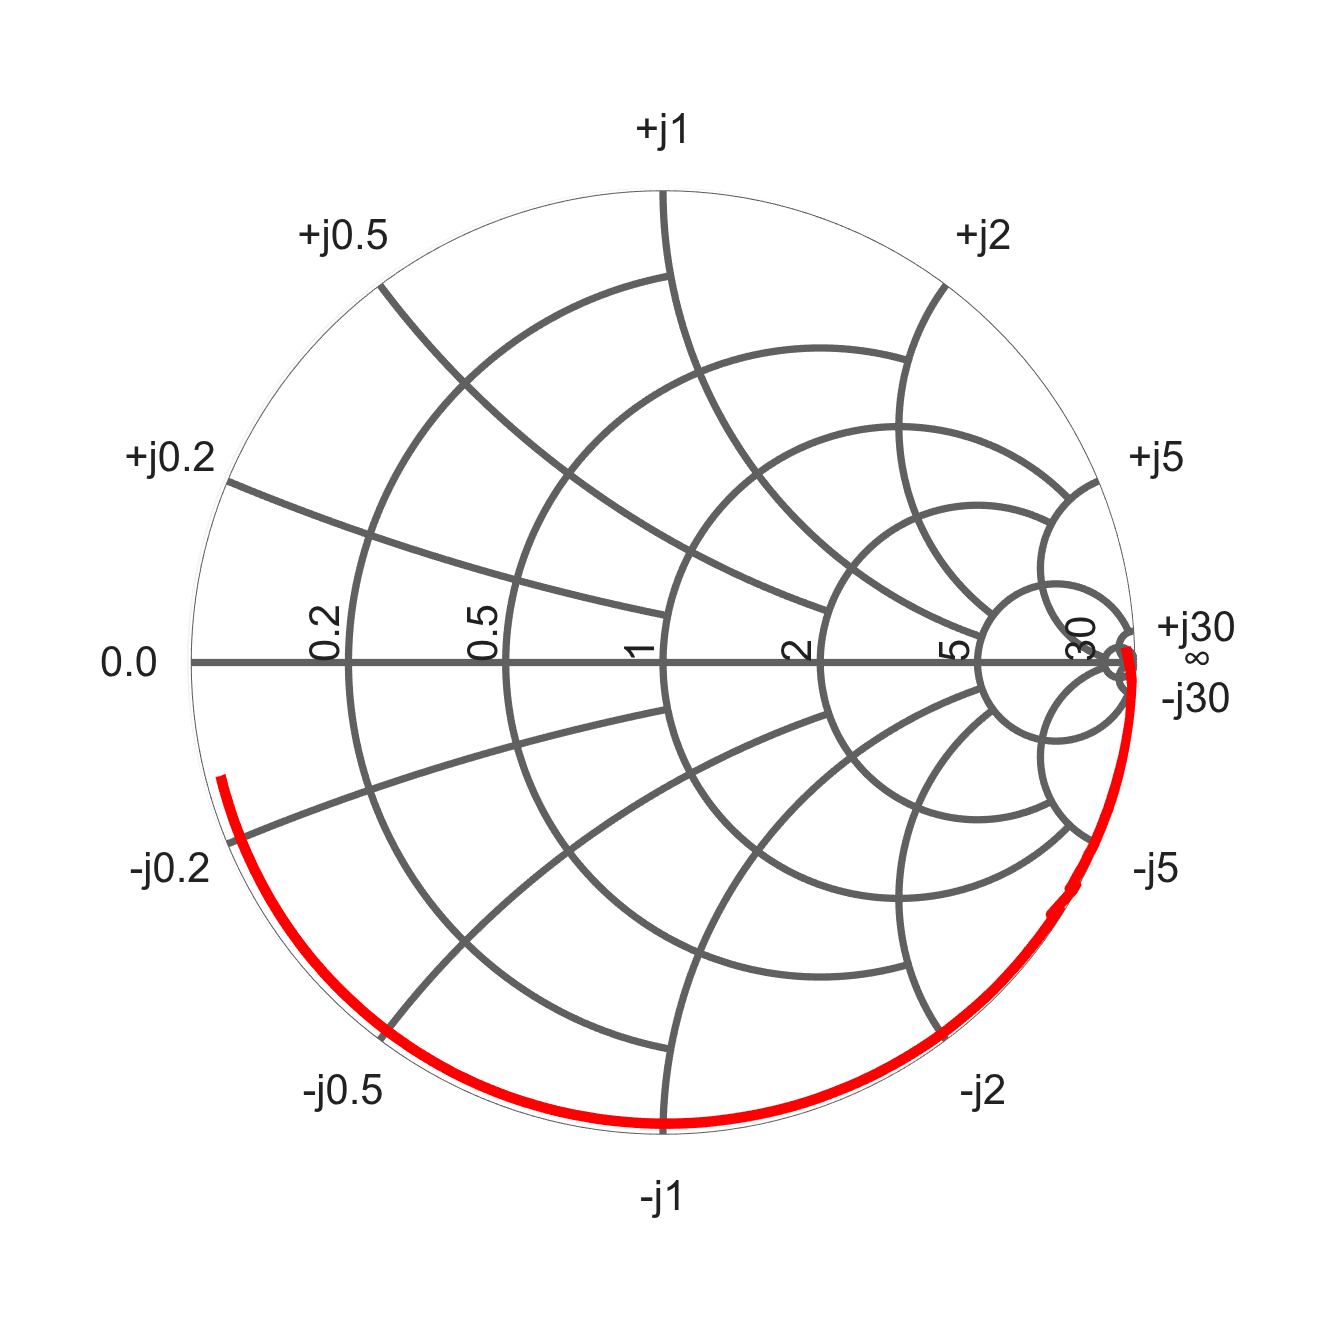
\includegraphics[width=0.4\textwidth]{./Images/Relazione1_Foto/7_1_microstrip_larga_aperto.png}
\caption{Smith chart con chiusura in circuito aperto misurata tra 1MHz e 100MHz.}
\end{figure}


Ripetendo la misura alla stessa frequenza, con la linea chiusa in corto circuito, abbiamo misurato:
\begin{equation}
Z_{SC}=0.6+j 20.32 \quad \Omega
\end{equation}
\begin{figure}[H]
  \centering
  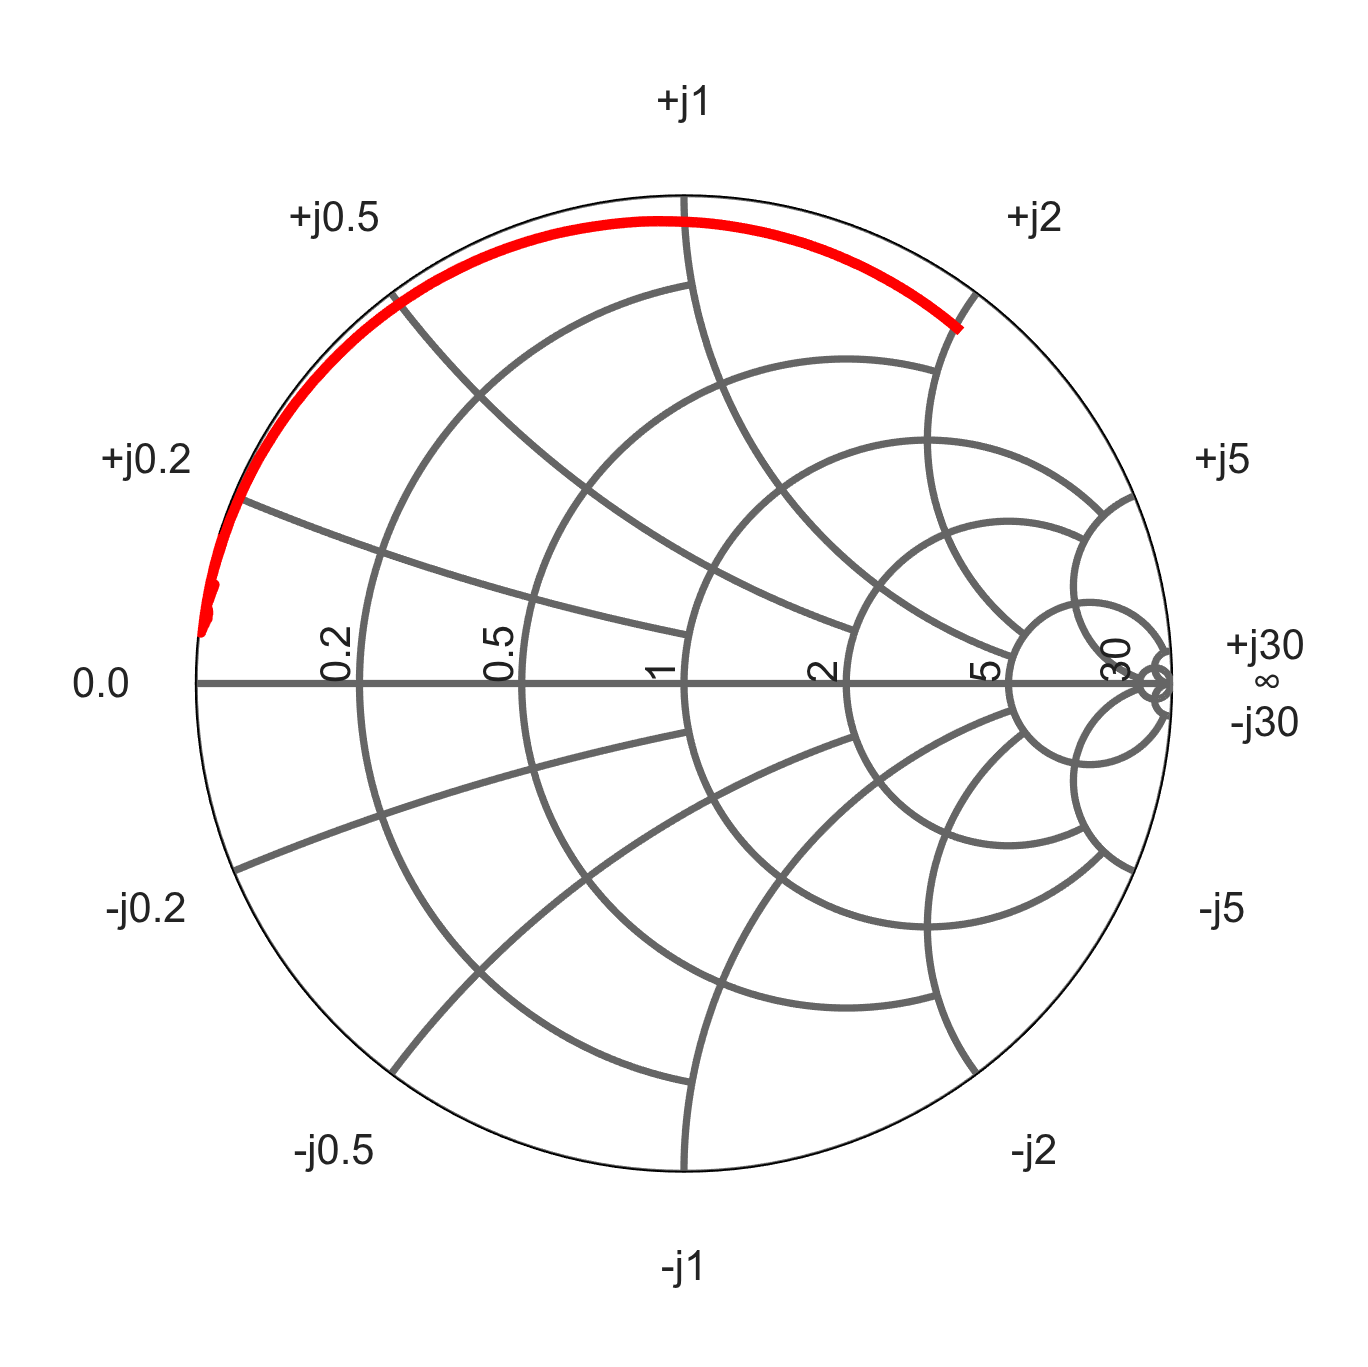
\includegraphics[width=0.4\textwidth]{./Images/Relazione1_Foto/7_1_microstrip_larga_corto.png}
\caption{Smith chart con chiusura in corto circuito misurata tra 1MHz e 100MHz.}
\end{figure}

Dalla teoria sappiamo che:
  \begin{align}
  Z_{SC} &= j\,Z_C \tan(\beta l) \\
  Z_{OC} &= -j\,Z_C \cot(\beta l) \\
  Z_C &= \sqrt{Z_{SC}\cdot Z_{OC}}
  \end{align}

Da queste misurazioni valutiamo l'impedenza caratteristica, trascurando le parti reali delle due impedenze dovute a non idealità e che sono molto minori rispetto alle parti immaginarie, come:
\begin{equation}
Z_C=\sqrt{Z_{OC}\cdot Z_{SC}}=25.5 \quad \Omega 
\end{equation}
Come si nota facilmente, le due misurazioni danno valori molto vicini tra loro.
\subsection{Microstriscia stretta}
Applichiamo i due metodi anche alla seconda microstriscia. Siamo partiti sempre dalla misurazione tramite la tecnica a "$\lambda/4$", e abbiamo ottenuto il seguente grafico:
\begin{figure}[H]
\centering
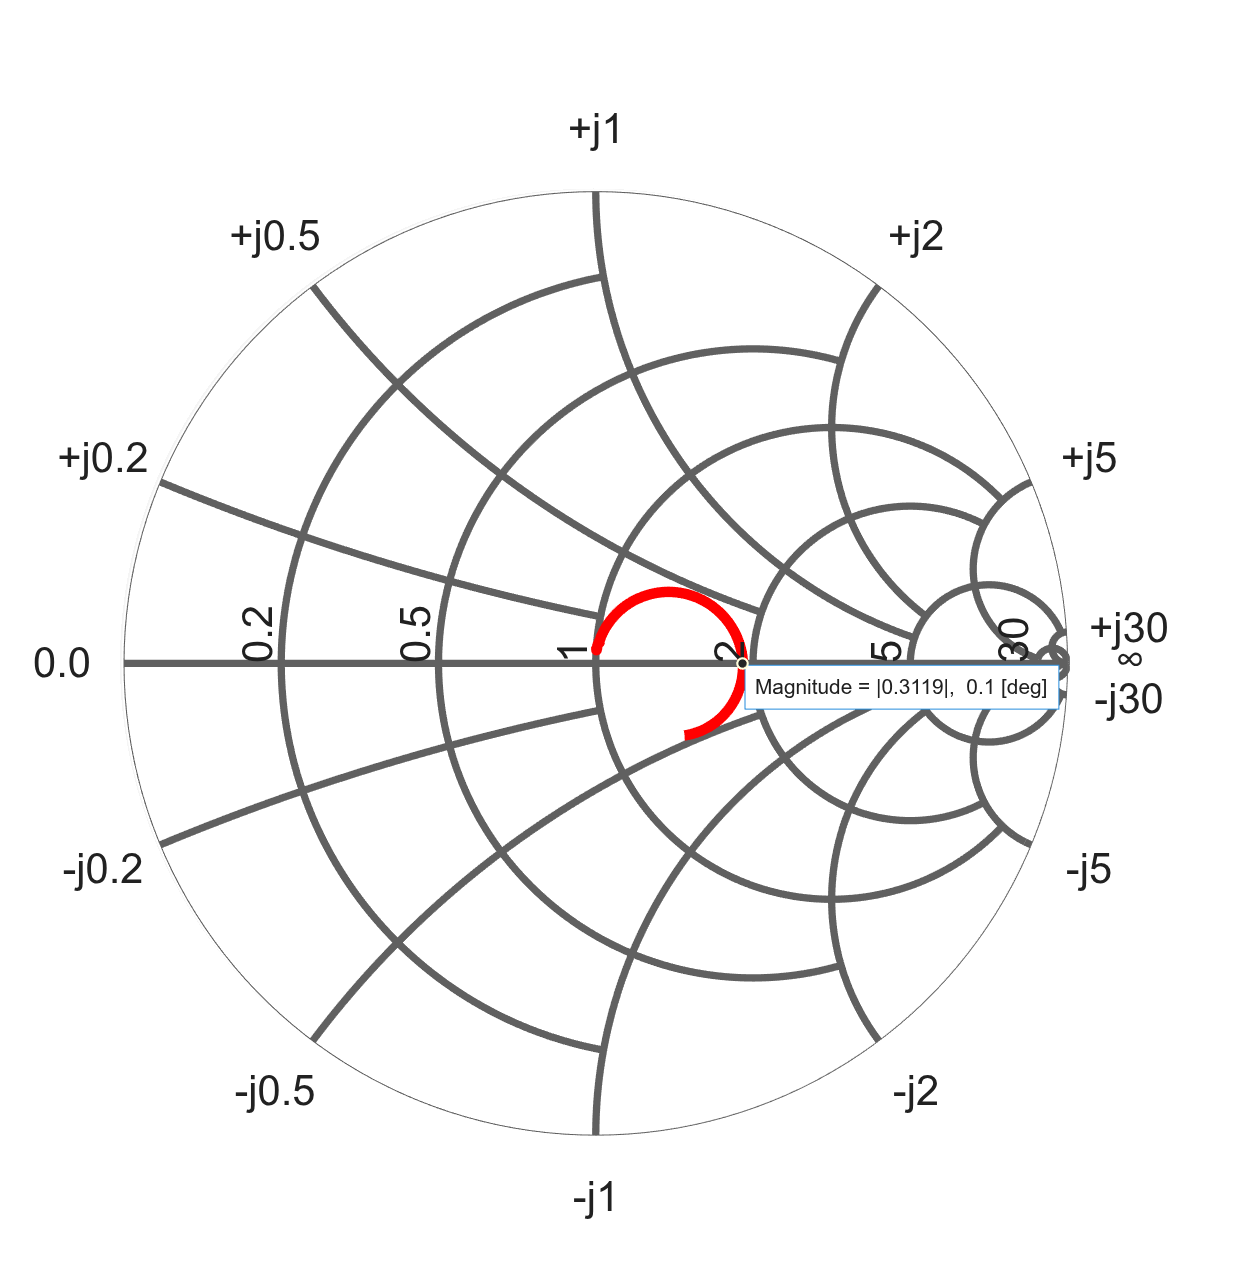
\includegraphics[width=0.4\textwidth]{./Images/Relazione1_Foto/7_1_microstrip_stretta_lambda_quarti.png}
\caption{Smith chart dell'impedenza tramite tecnica "$\lambda/4$".}
\end{figure}
Il valore misurato è:
\begin{equation}
Z_{IN}=95.36 - j0.4 \quad \Omega
\end{equation}
E quindi ricaviamo:
\begin{equation}
Z_C=\sqrt{Z_{IN}\cdot Z_0}=\sqrt{95.36\cdot50}\simeq 69.05 \quad \Omega
\end{equation}

Anche in questo caso passiamo a valutare l'impedenza caratteristica tramite la tecnica di misura "corto circuito-
circuito aperto". Abbiamo ottenuto i seguenti valori, presi a 81.2MHz, frequenza alla quale, nella misura in circuito aperto, la parte reale è minima, con span tra 2MHz e 200MHz:
\begin{equation}
Z_{OC}=1.79-j46.37 \quad \Omega
\end{equation}
\begin{figure}[H]
  \centering
  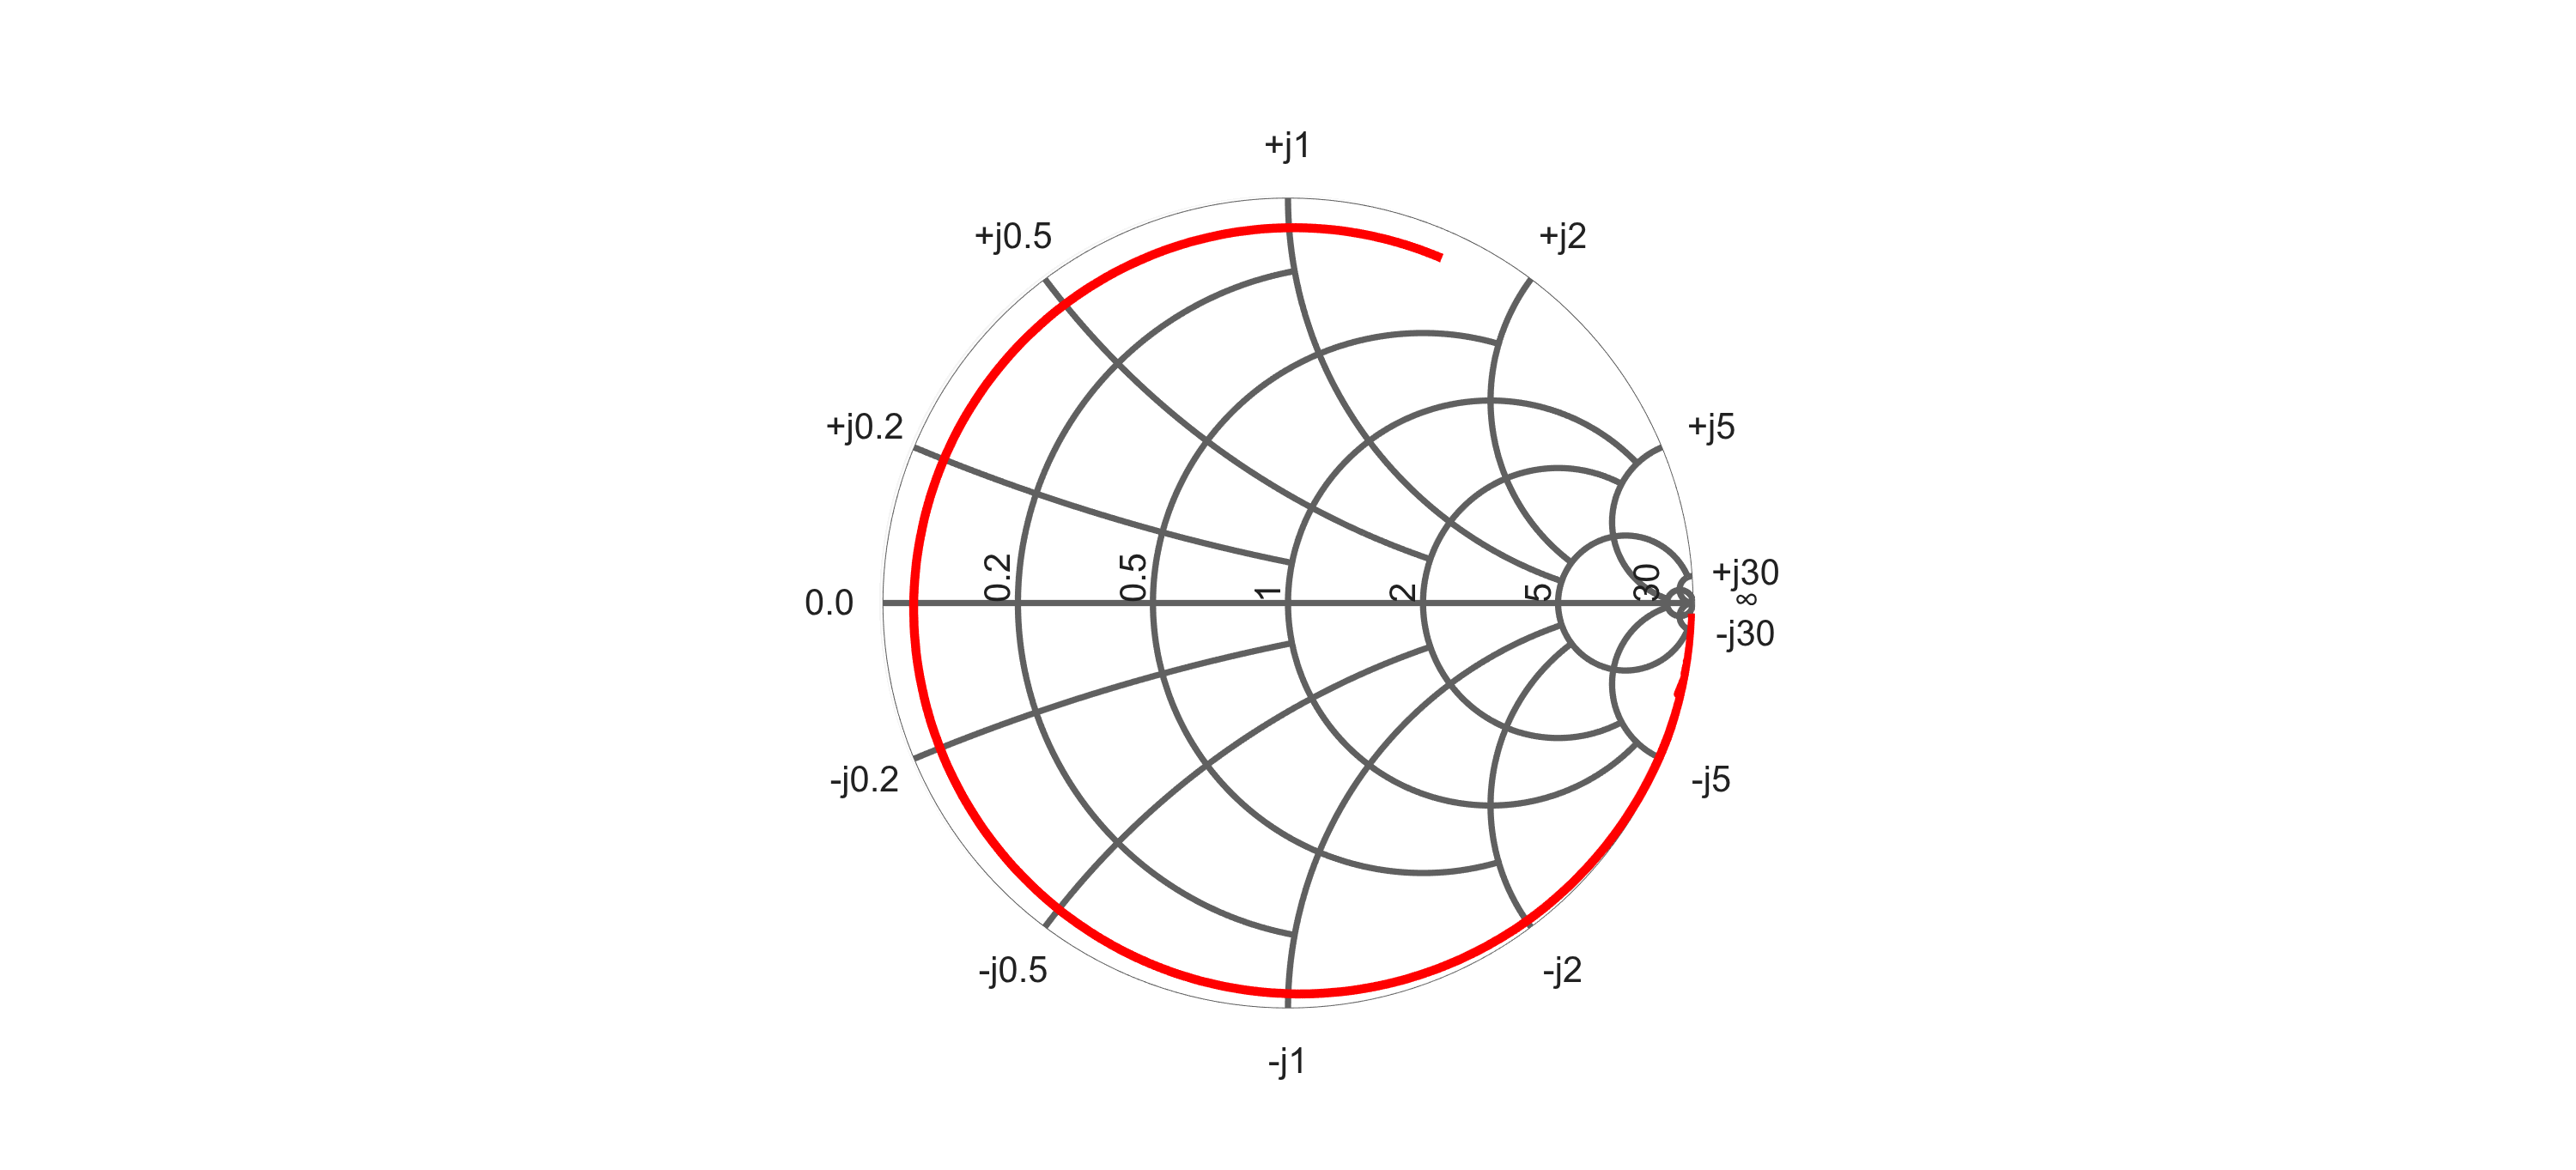
\includegraphics[width=0.8\textwidth]{./Images/Relazione1_Foto/7_1_microstrip_stretta_open.png}
\caption{Smith chart con chiusura in circuito aperto misurata tra 2MHz e 200MHz.}
\end{figure}

\begin{equation}
Z_{SC}=6.76+j 103.56 \quad \Omega
\end{equation}
\begin{figure}[H]
  \centering
  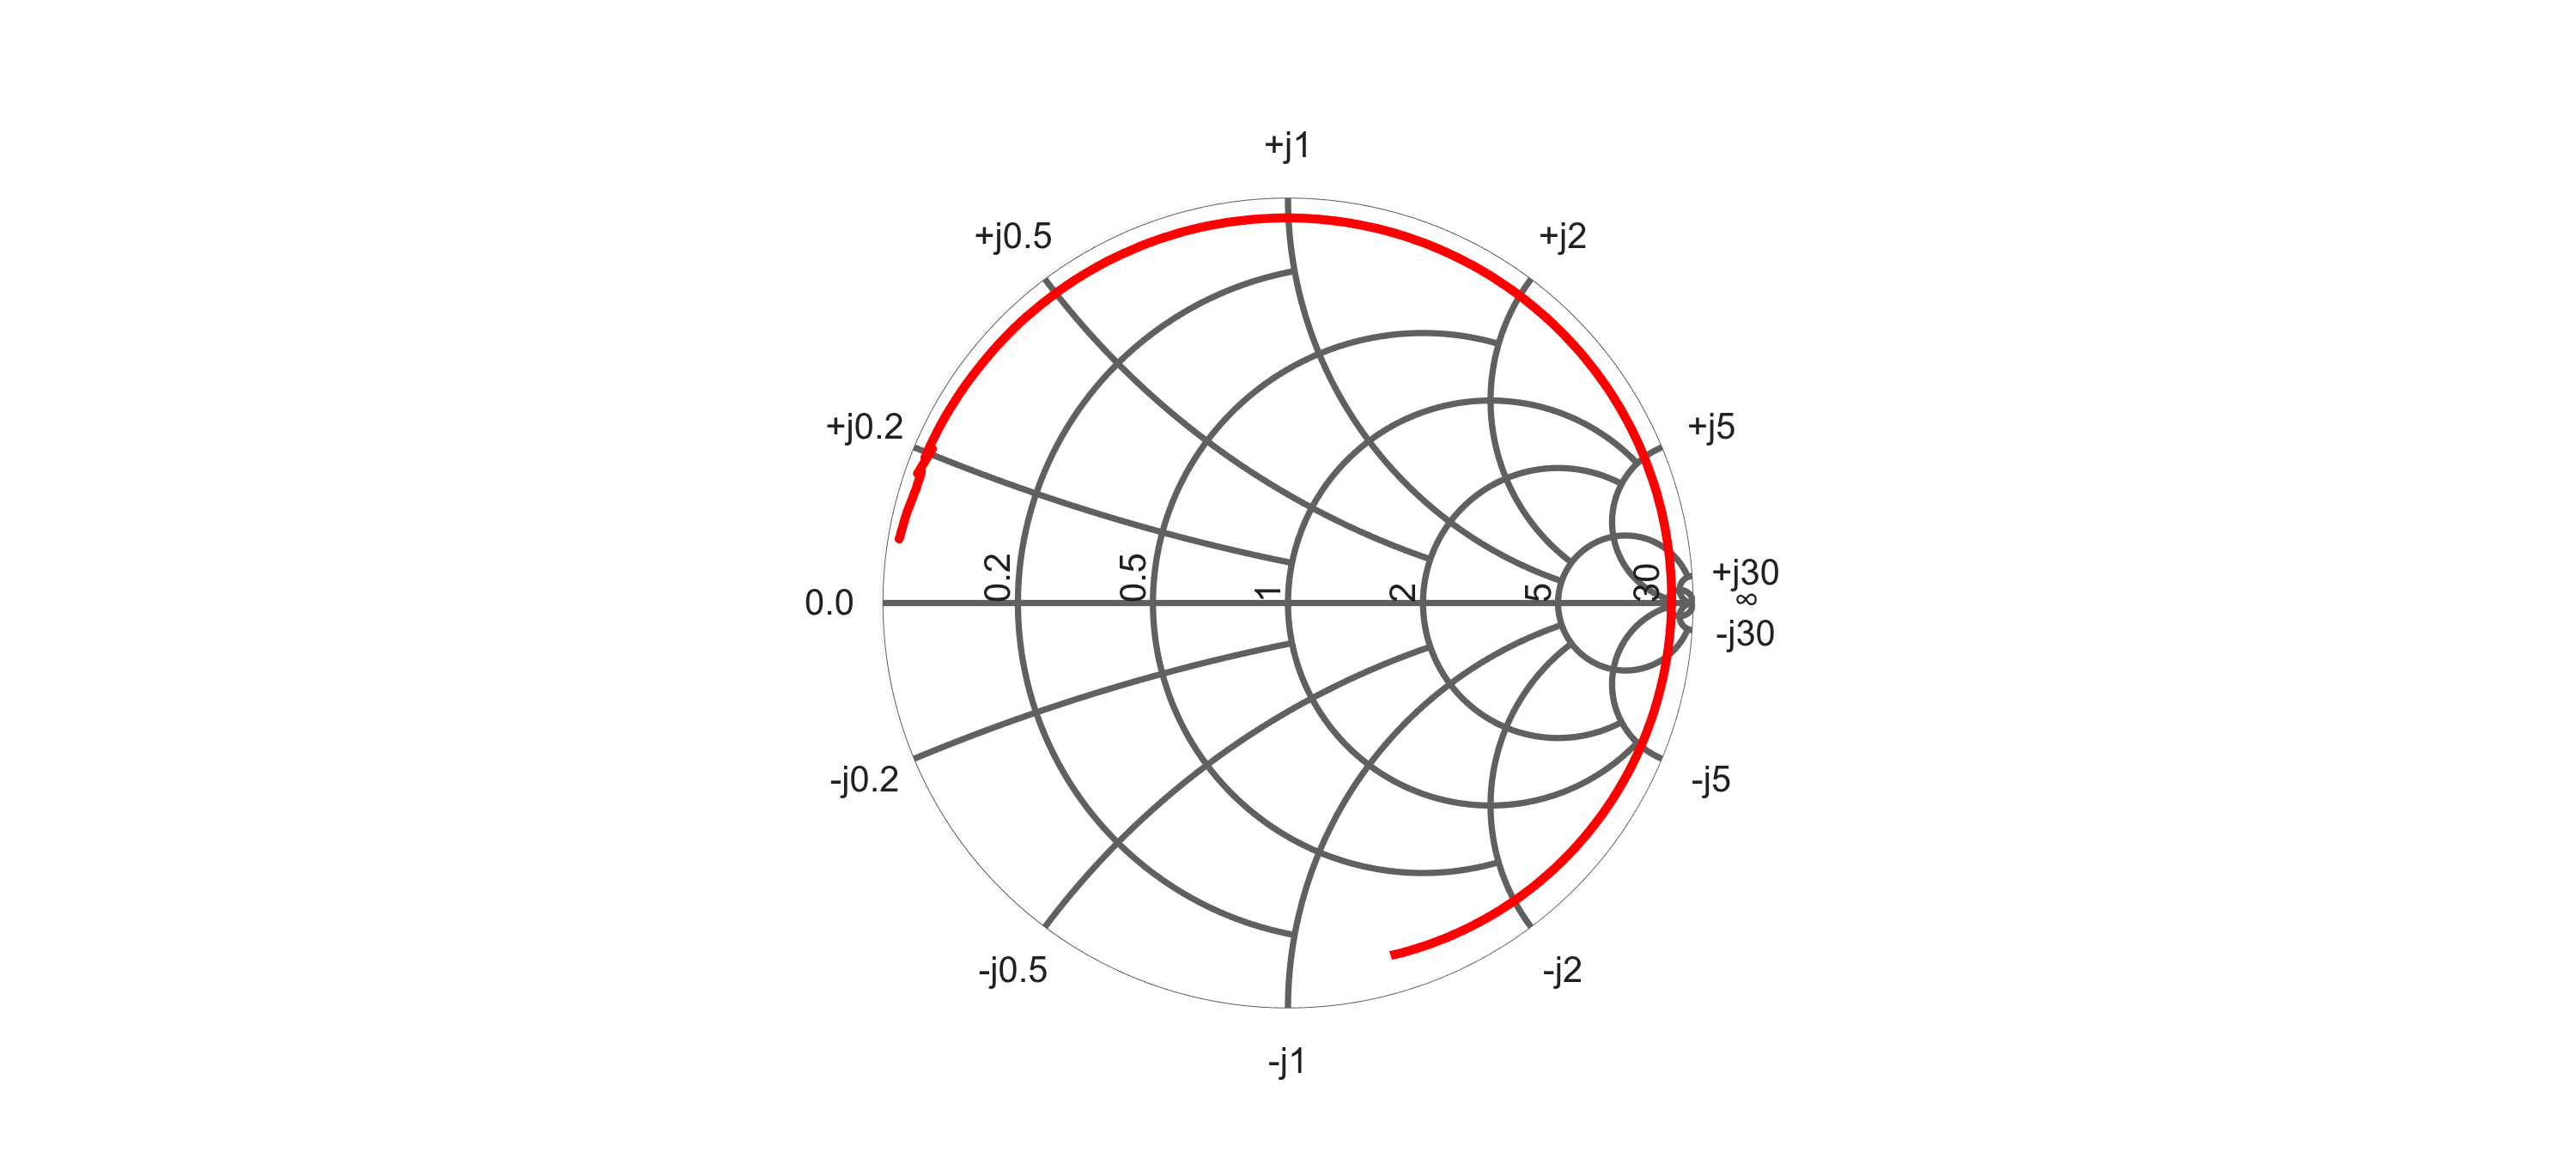
\includegraphics[width=0.8\textwidth]{./Images/Relazione1_Foto/7_1_microstrip_stretta_short.png}
\caption{Smith chart con chiusura in corto circuito misurata tra 2MHz e 200MHz.}
\end{figure}
Quindi l'impedenza caratteristica misurata con questo metodo è (trascurando anche qui le parti reali, nettamente inferiori rispetto alle parti immaginarie, e dovute a non idealità):
\begin{equation}
  Z_{C}=\sqrt{Z_{SC}\cdot Z_{OC}}\simeq 69.30 \quad \Omega
\end{equation}
Anche in questo caso si può notare che le due impedenze sono molto vicine tra loro.

\section{Misura della permettività}
Date le due microstrisce precedenti, vogliamo misurare la loro permettività. Per farlo esistono vari
metodi; tra questi noi abbiamo scelto di usare la misura del parametro di trasmissione $S_{21}$.
Come nel capitolo 4 abbiamo misurato la fase di $S_{21}$ in formato unwrapped, e abbiamo aggiunto dallo
strumento un electrical delay che portasse la fase circa a 0 (non esattamente, ovviamente, per via della presenza di una dipendenza non lineare della 
fase dalla frequenza e poiché il metodo per basse frequenze perde validità).
\subsection{Microstriscia stretta}
Nel primo caso abbiamo annullato la fase con un electrical delay di 1.81 ns.
\begin{figure}[H]
  \centering
  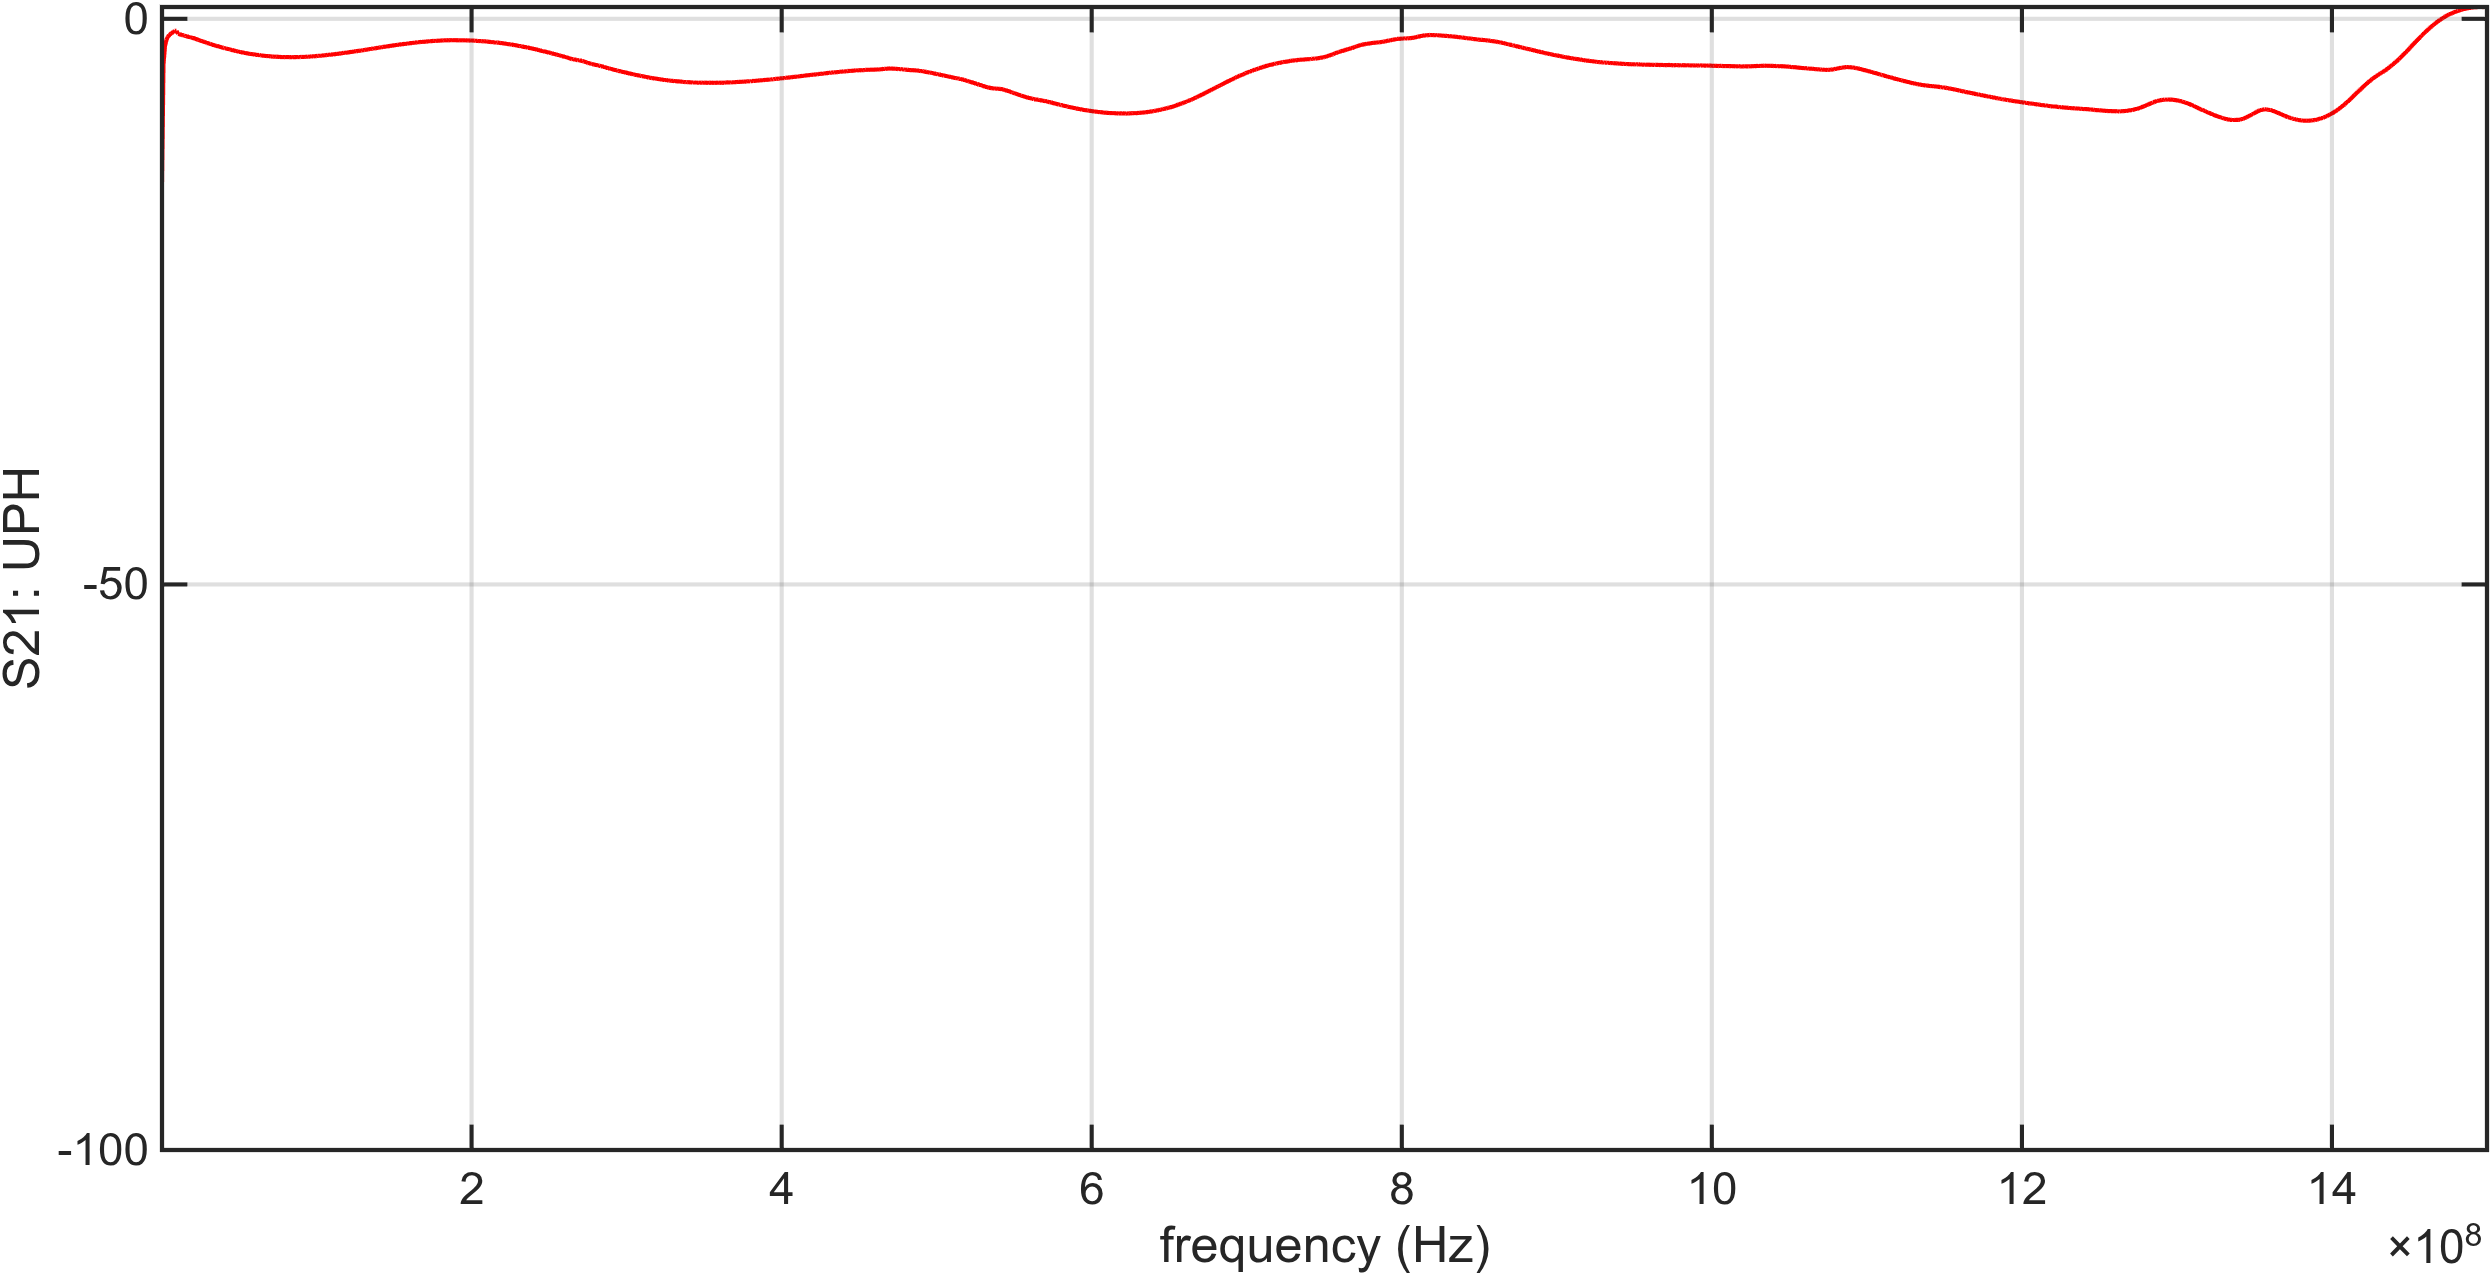
\includegraphics[width=0.6\textwidth]{./Images/Relazione1_Foto/7_2_fase_microstrip_stretta.png}
  \caption{Grafico della fase di $S_{21}$ con electrical delay di 1.81 ns.}
\end{figure}
A partire dall'electrical delay, $\tau$, abbiamo poi:
\begin{equation}
  L_0=c \tau=3\cdot 10^8\cdot1.81\cdot 10^{-9}=0.543\ \mathrm{m}
\end{equation}
Dalla $L_0$, lunghezza nel vuoto, ricaviamo la permettività dalla lunghezza effettiva, pari a 29.5 cm.
\begin{align}
  n &=\sqrt{\epsilon_r}=\frac{L_0}{L}=1.8407 \\
  \epsilon_r &= n^2=3.3881
\end{align}

\subsection{Microstriscia larga}
In questo caso abbiamo annullato la fase con un electrical delay di 1.991 ns.
\begin{figure}[H]
  \centering
  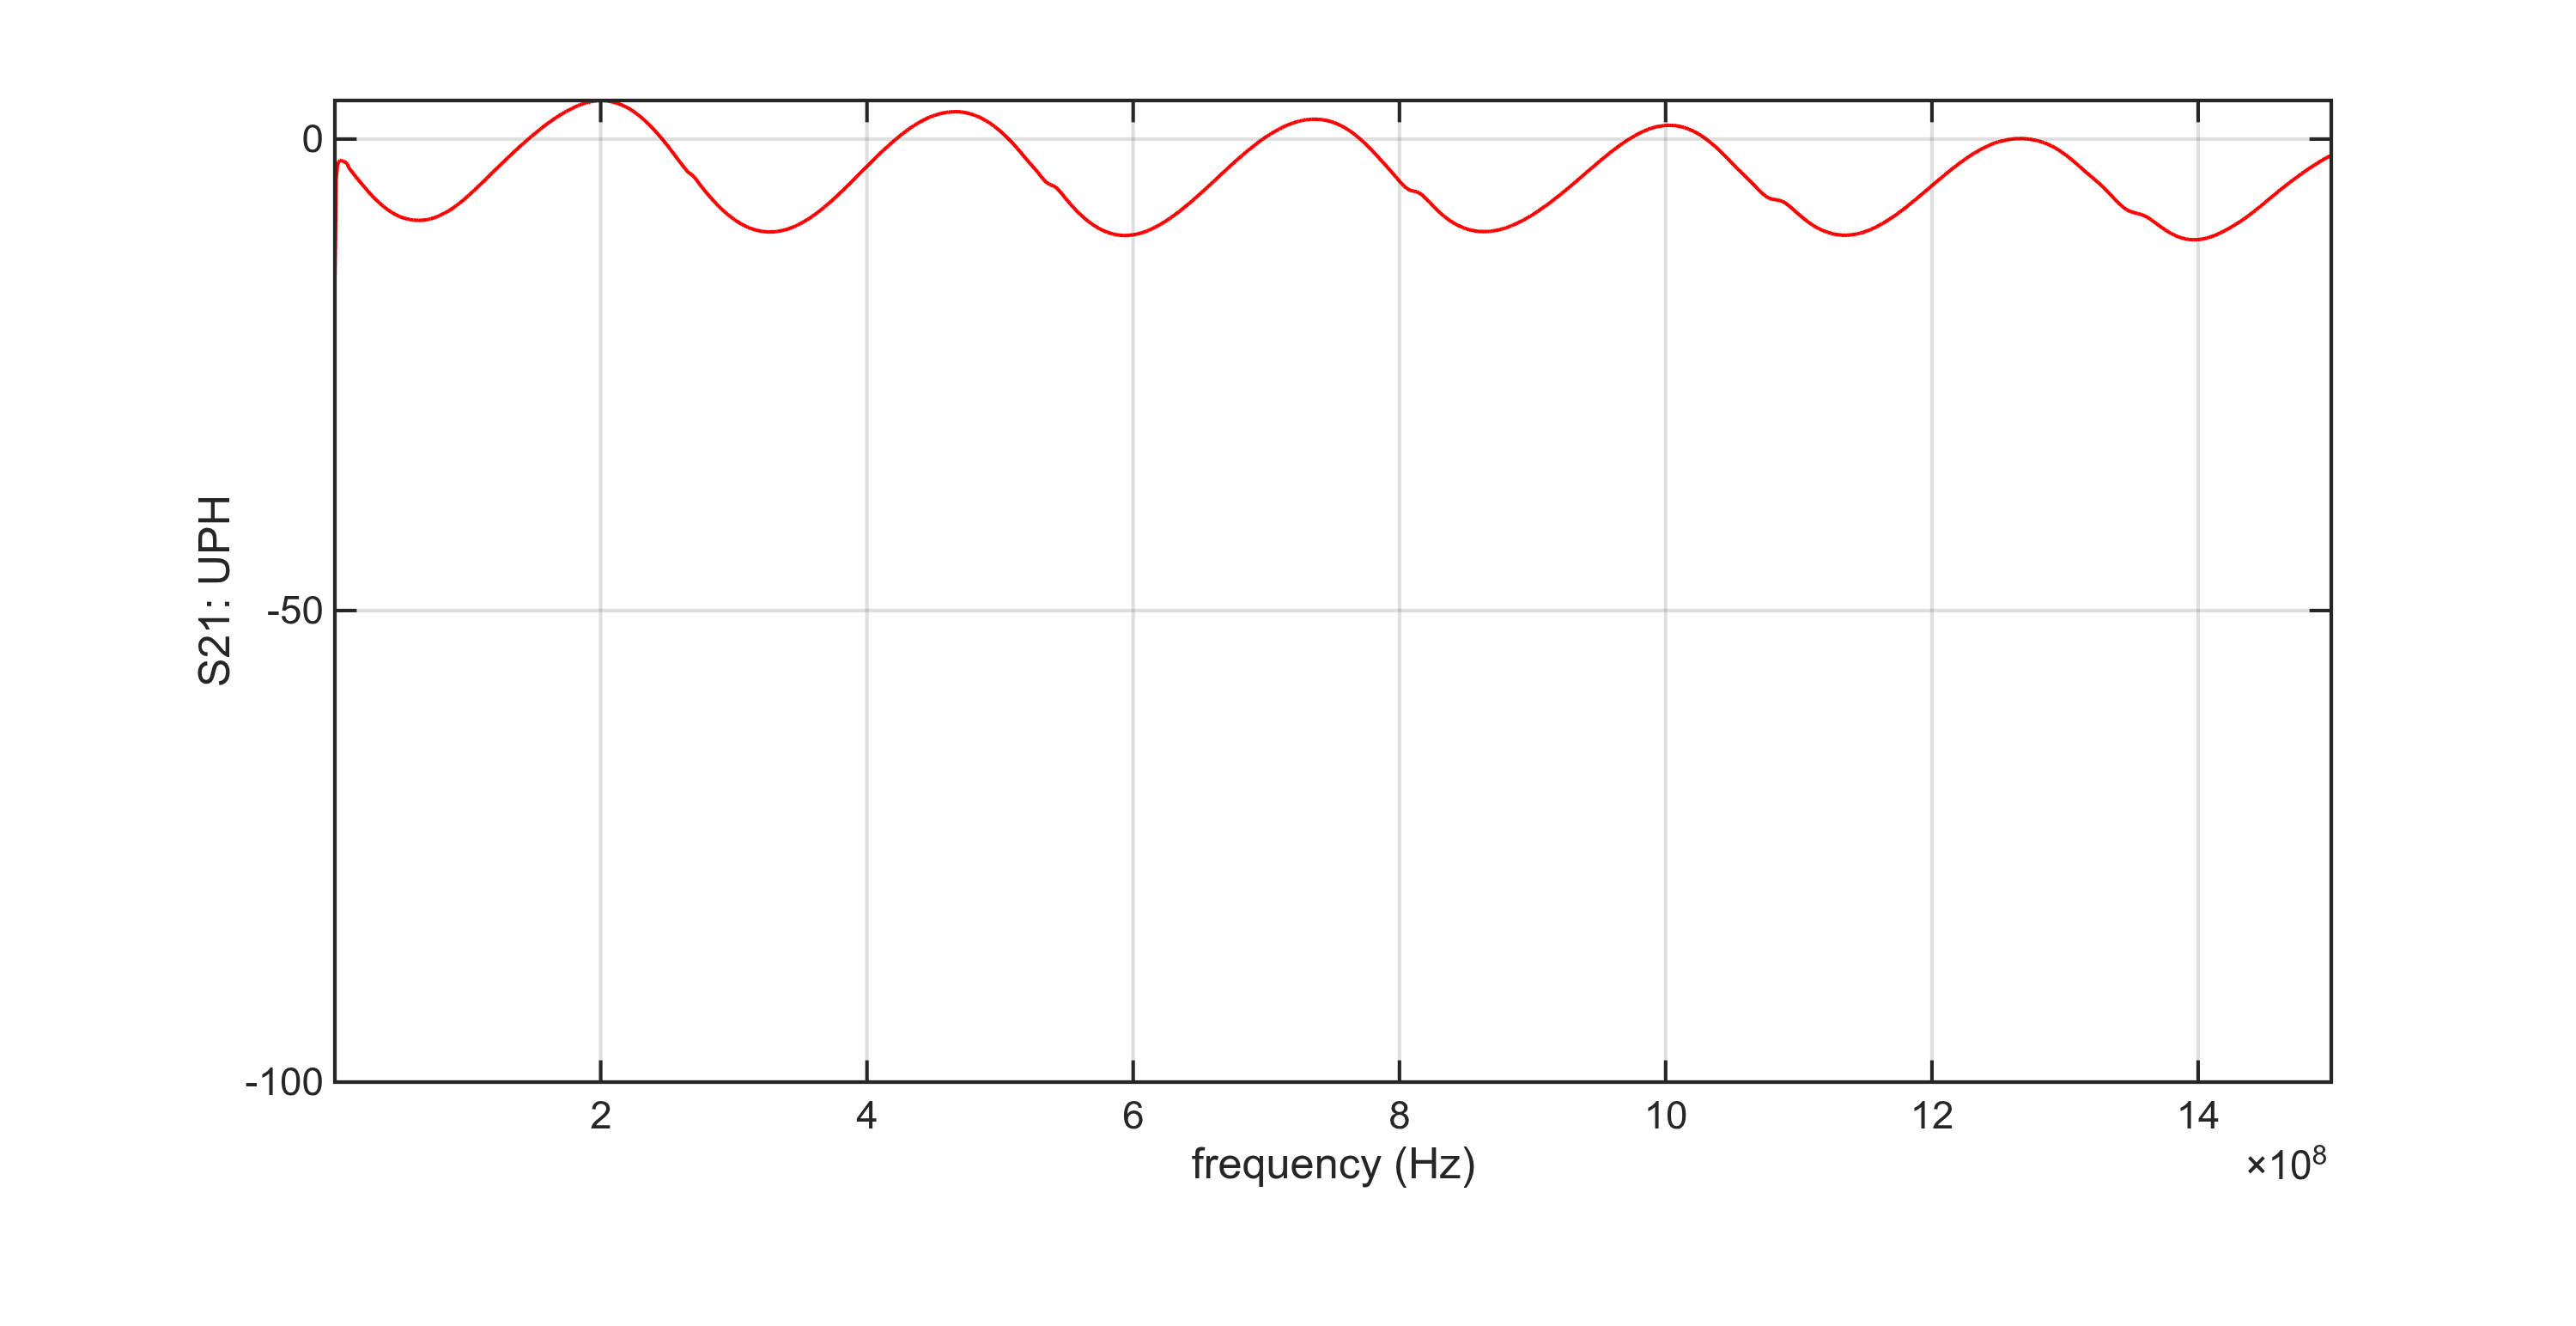
\includegraphics[width=0.6\textwidth]{./Images/Relazione1_Foto/7_2_fase_microstrip_larga.png}
  \caption{Grafico della fase di $S_{21}$ con electrical delay di 1.991 ns.}
\end{figure}
A partire dall'electrical delay, $\tau$, abbiamo poi:
\begin{equation}
  L_0=c \tau=3\cdot 10^8\cdot1.991\cdot 10^{-9}= 0.5973\ \mathrm{m}
\end{equation}
Dalla $L_0$, lunghezza nel vuoto, ricaviamo la permettività dalla lunghezza effettiva, pari a 29.5 cm.
\begin{align}
  n &=\sqrt{\epsilon_r}=\frac{L_0}{L}=    2.0247 \\
  \epsilon_r &= n^2=    4.0996
\end{align}

% =====================================================================
% Capitolo 8
% =====================================================================
\chapter{Costante di propagazione di una guida d'onda per il modo TE10}
\section{Misura della costante di propagazione}
Tramite lo strumento abbiamo misurato la fase di $S_{21}$ per valutare il comportamento
della costante di propagazione in funzione della frequenza. 

\begin{figure}[H]
  \centering
  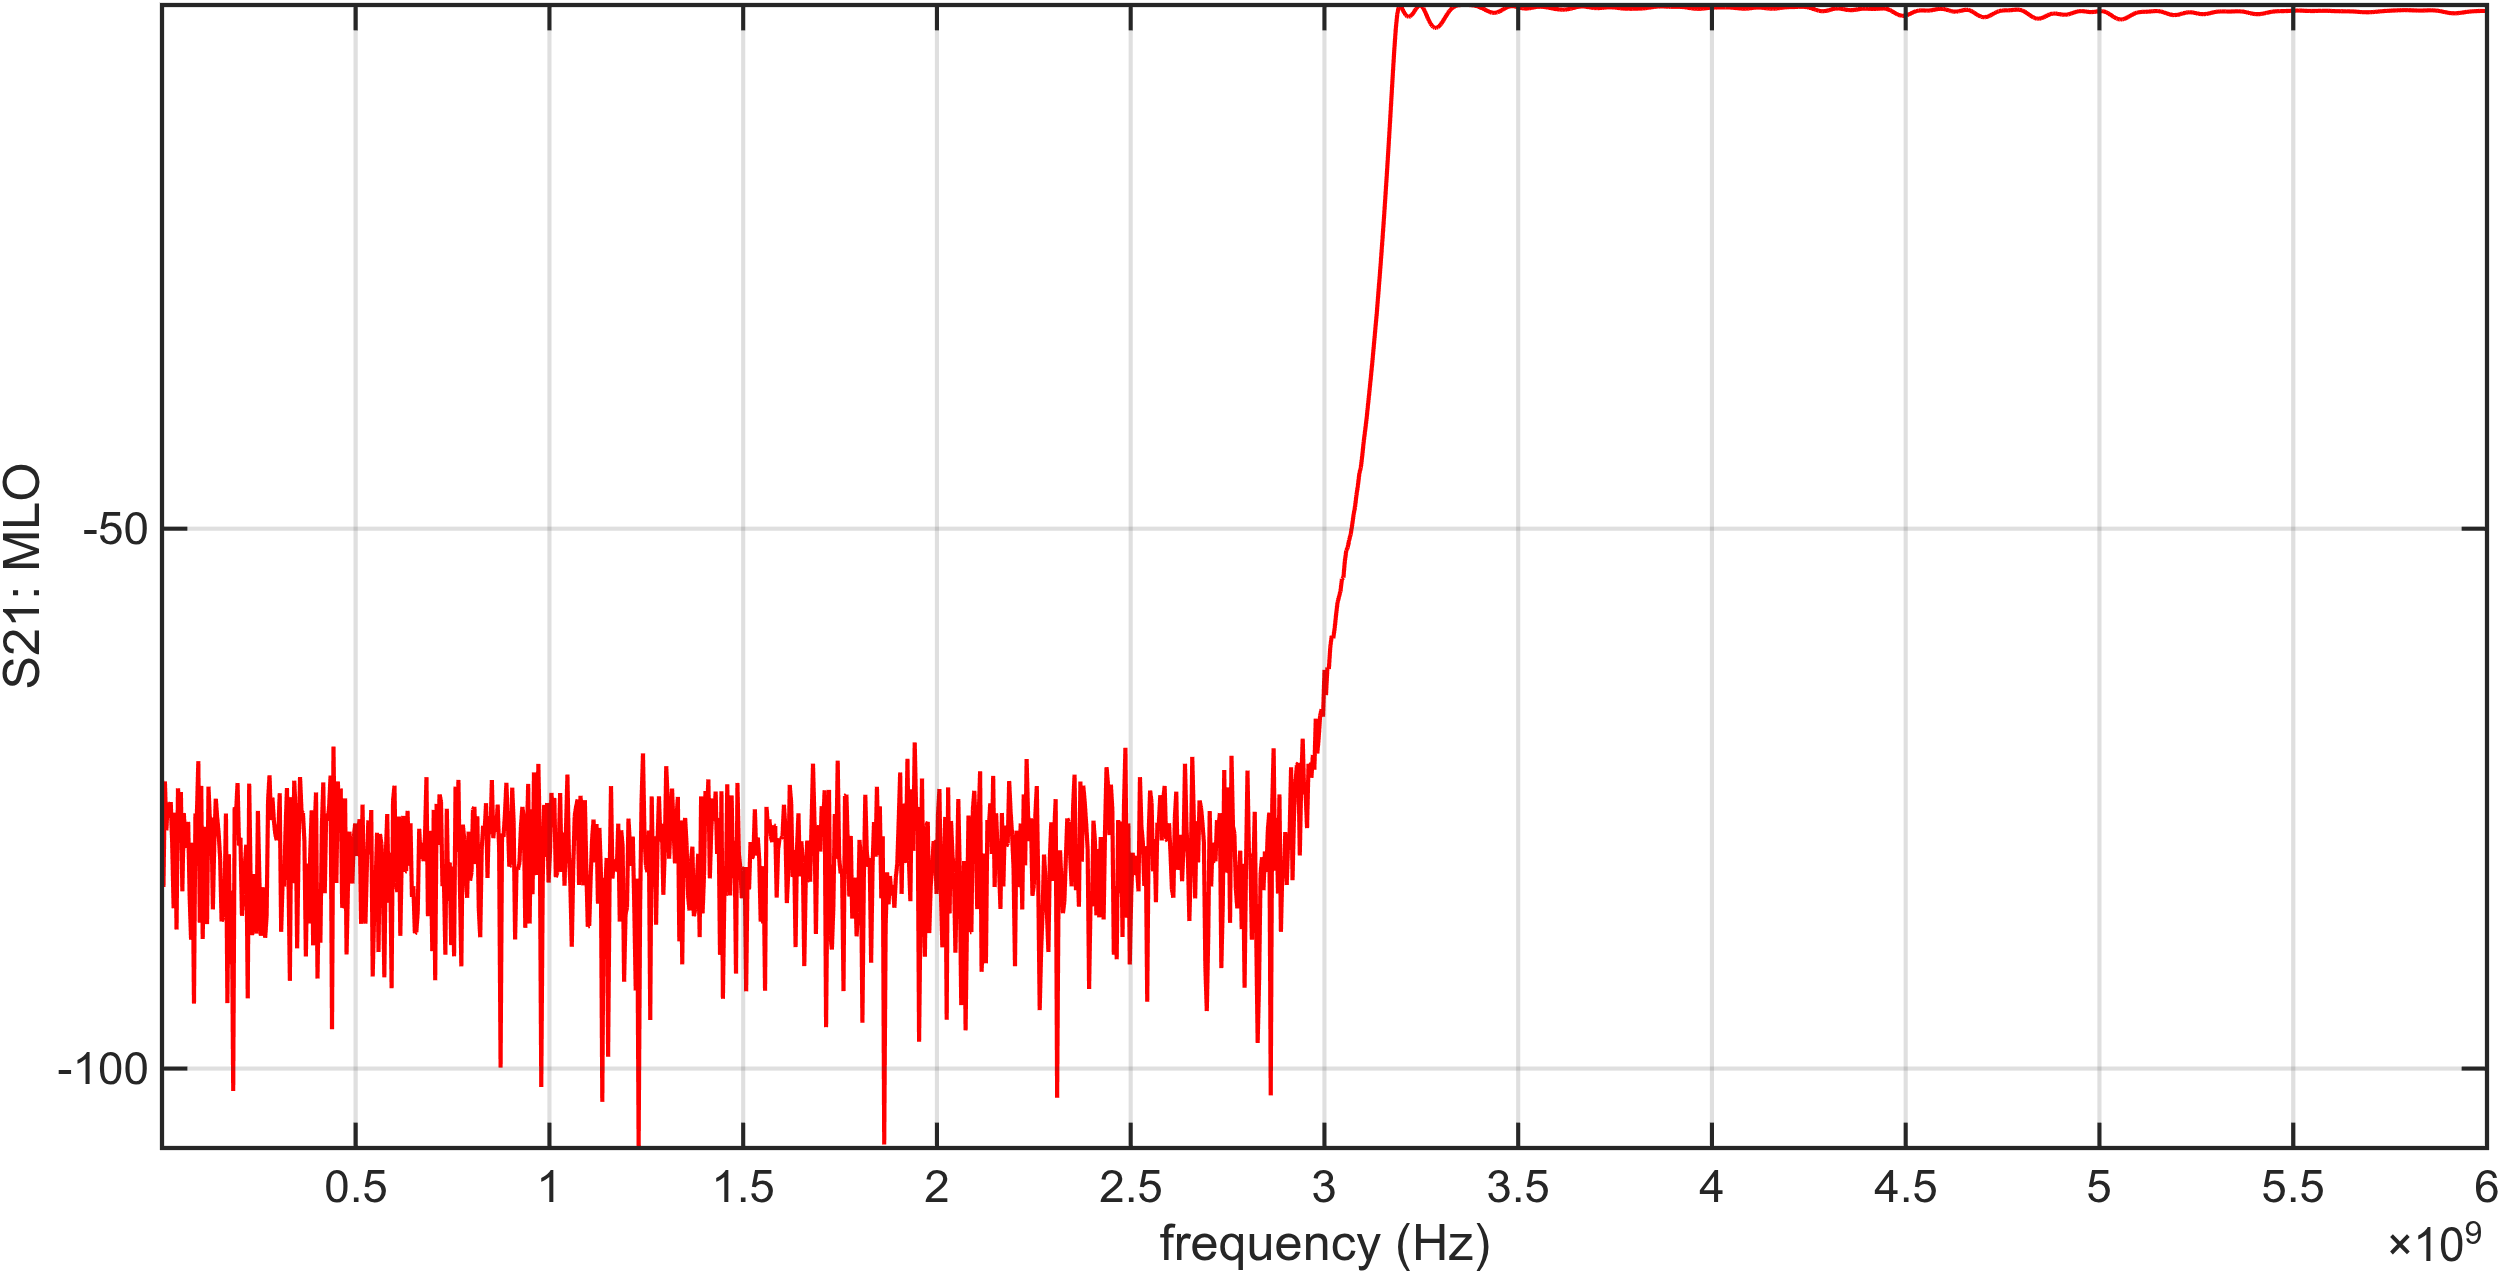
\includegraphics[width=0.6\textwidth]{./Images/Relazione1_Foto/8_1_fase_S21_modo_guida.png}
  \caption{Andamento in frequenza della fase di $S_{21}$ tra 0 e 6 GHz.}
\end{figure}


\begin{figure}[H]
  \centering
  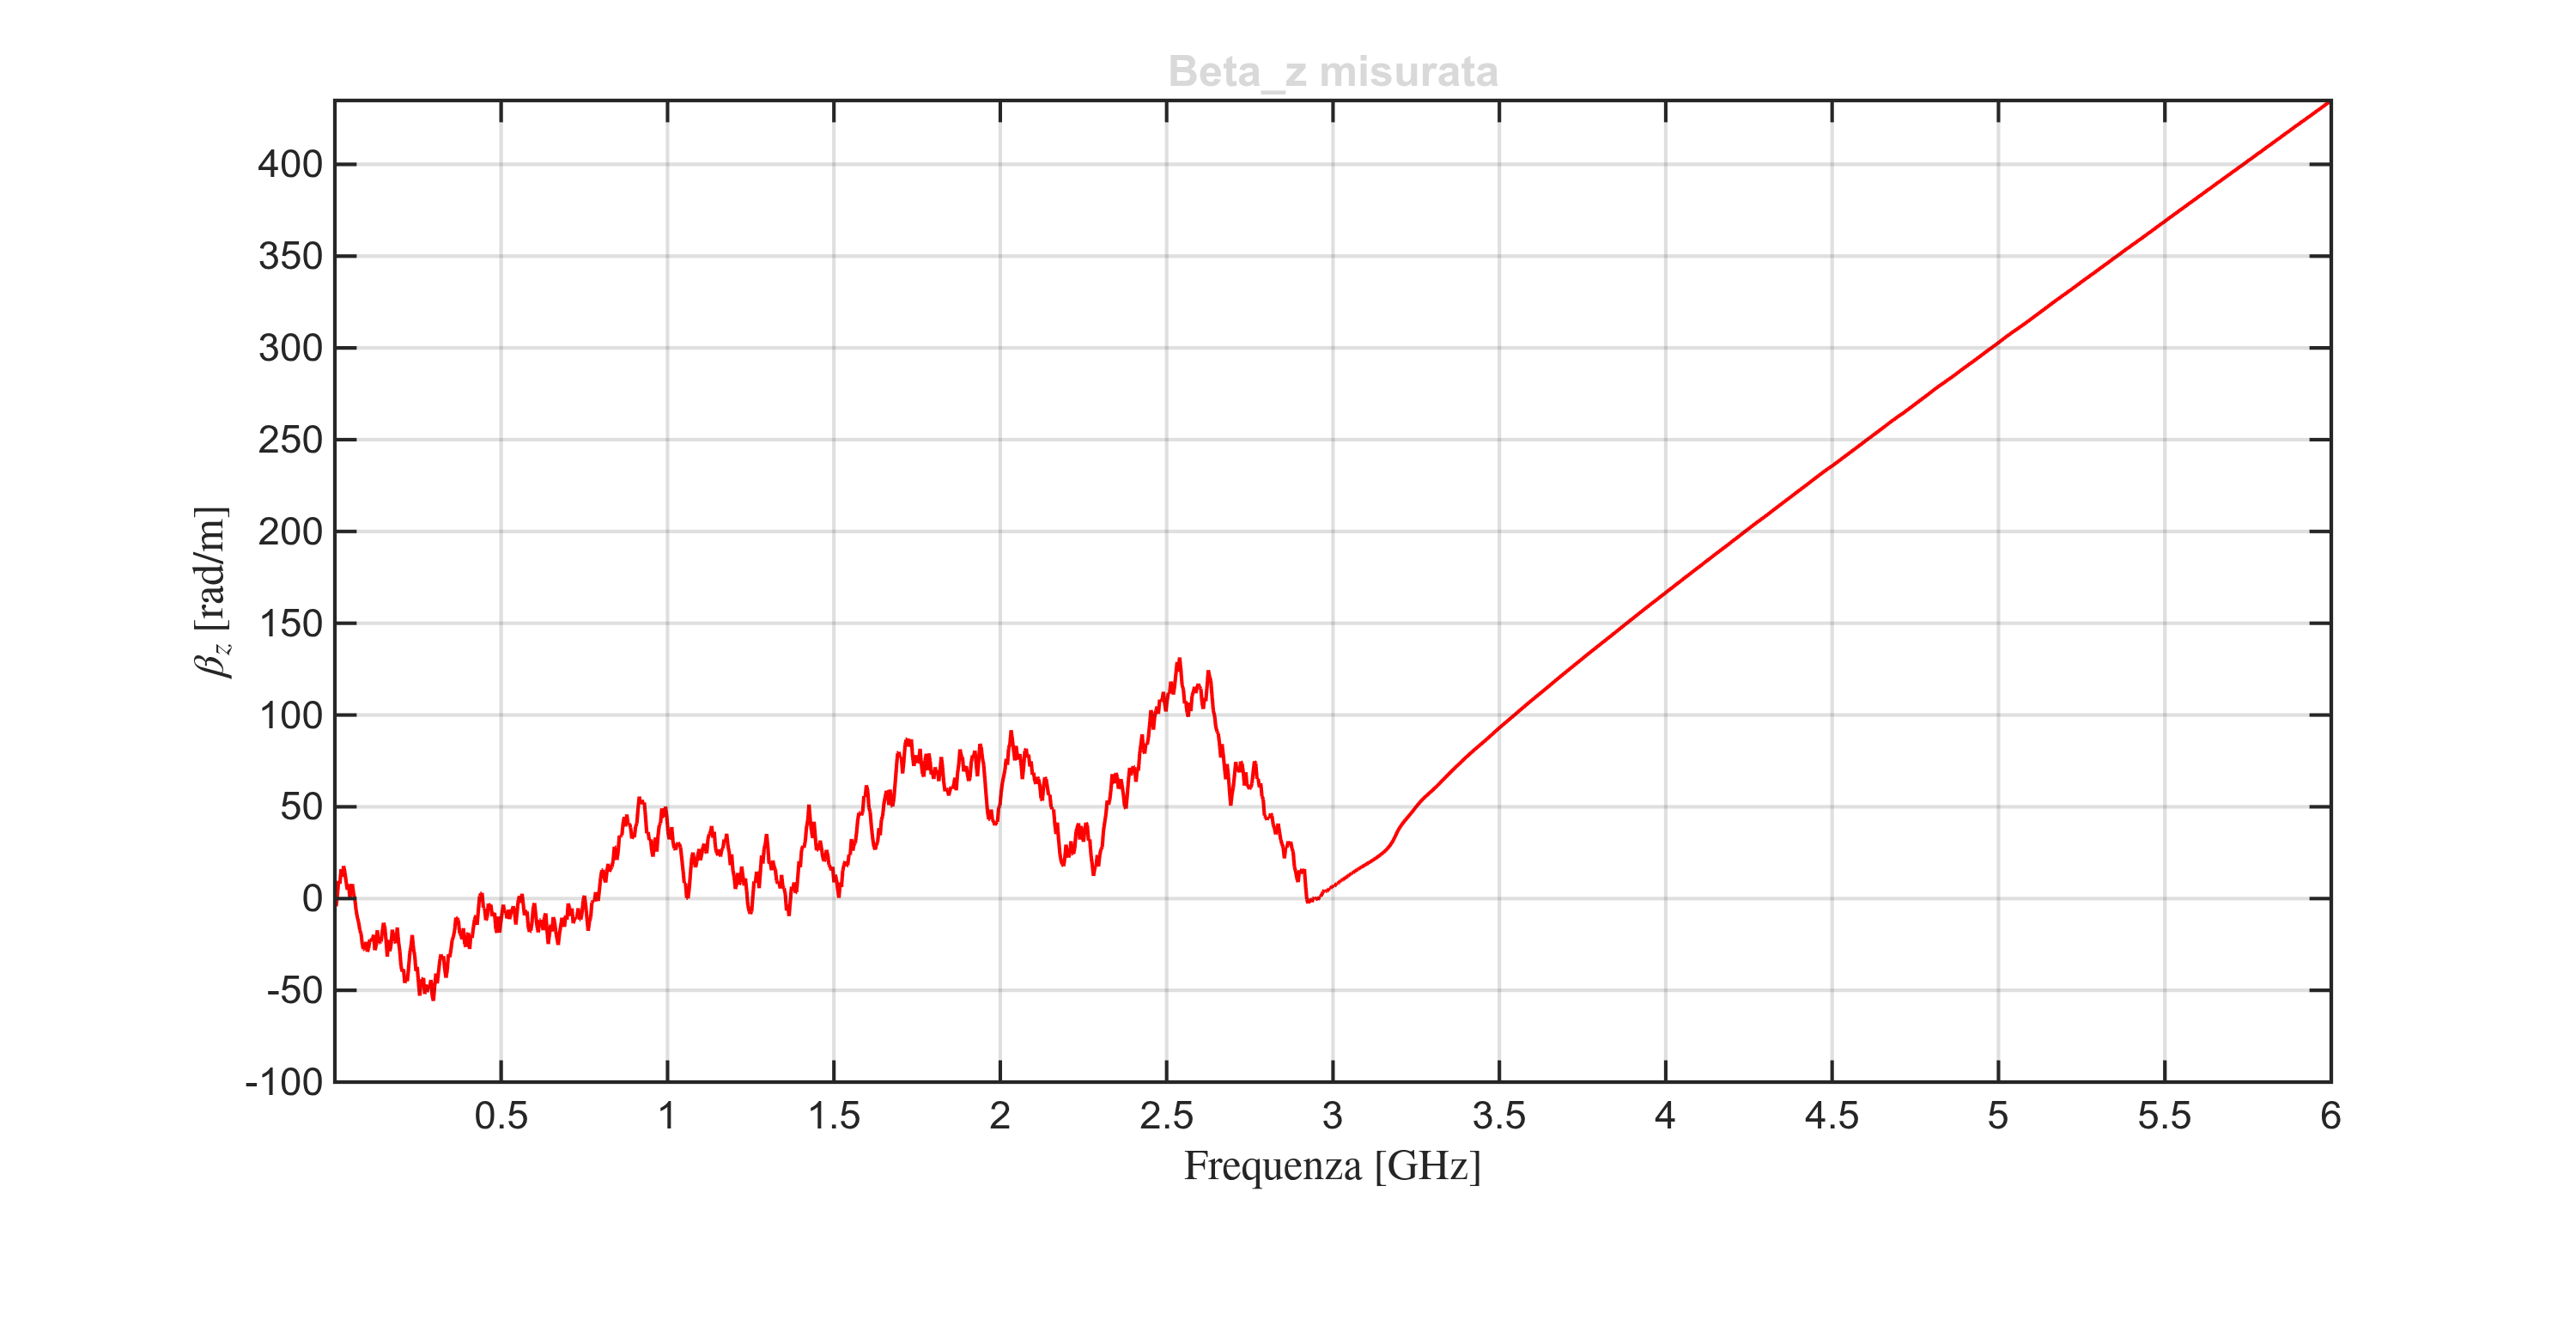
\includegraphics[width=0.7\textwidth]{./Images/Relazione1_Foto/8_2_fase_beta_zeta_misurato.png}
  \caption{Andamento in frequenza della costante di propagazione tra 0 e 6 GHz.}
\end{figure}

Dalla teoria, per una guida d'onda rettangolare, sappiamo che il primo modo, il TE10, ha frequenza di cutoff pari a:
\begin{equation}
  f_{c,10}=\frac{c}{2a}=\frac{3\cdot 10^8}{2\cdot 0.04755}=   3.1546 \cdot 10^9\ \mathrm{Hz}
\end{equation}
dove $a$ è il lato più lungo della guida.
La costante di propagazione $\beta_z$ è:
\begin{equation}
  \beta_z = \sqrt{\left(\frac{2\pi f}{c}\right)^2 - \left(\frac{\pi}{a}\right)^2}
\end{equation}
Di seguito il grafico con $\beta_z$ teorico e misurato confrontati.
\begin{figure}[H]
  \centering
  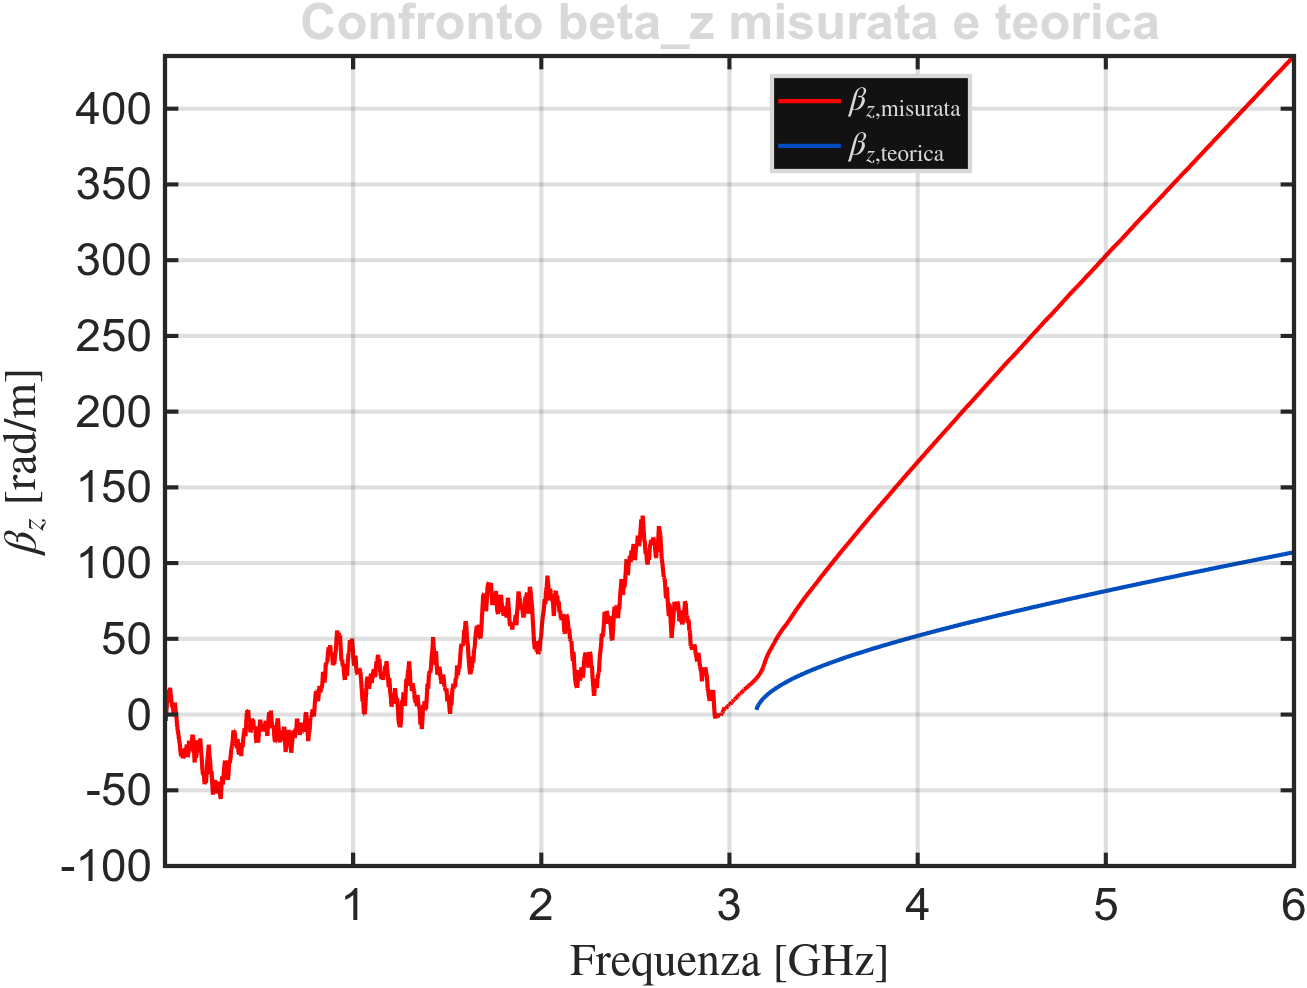
\includegraphics[width=0.6\textwidth]{./Images/Relazione1_Foto/8_2_grafico_beta_mixed.png}
  \caption{Grafico della costante di propagazione misurata e teorica tra 0 e 6GHz.}
\end{figure}

\section{Misura di \texorpdfstring{$S_{11}$}{S11} con carico adattato}
Siamo passati a valutare il coefficiente di riflessione mettendo il carico adattato ad un estremo della guida.

Il carico è progettato per funzionare a 5.712 GHz. Il grafico della $S_{11}$ è il seguente:
\begin{figure}[H]
  \centering
  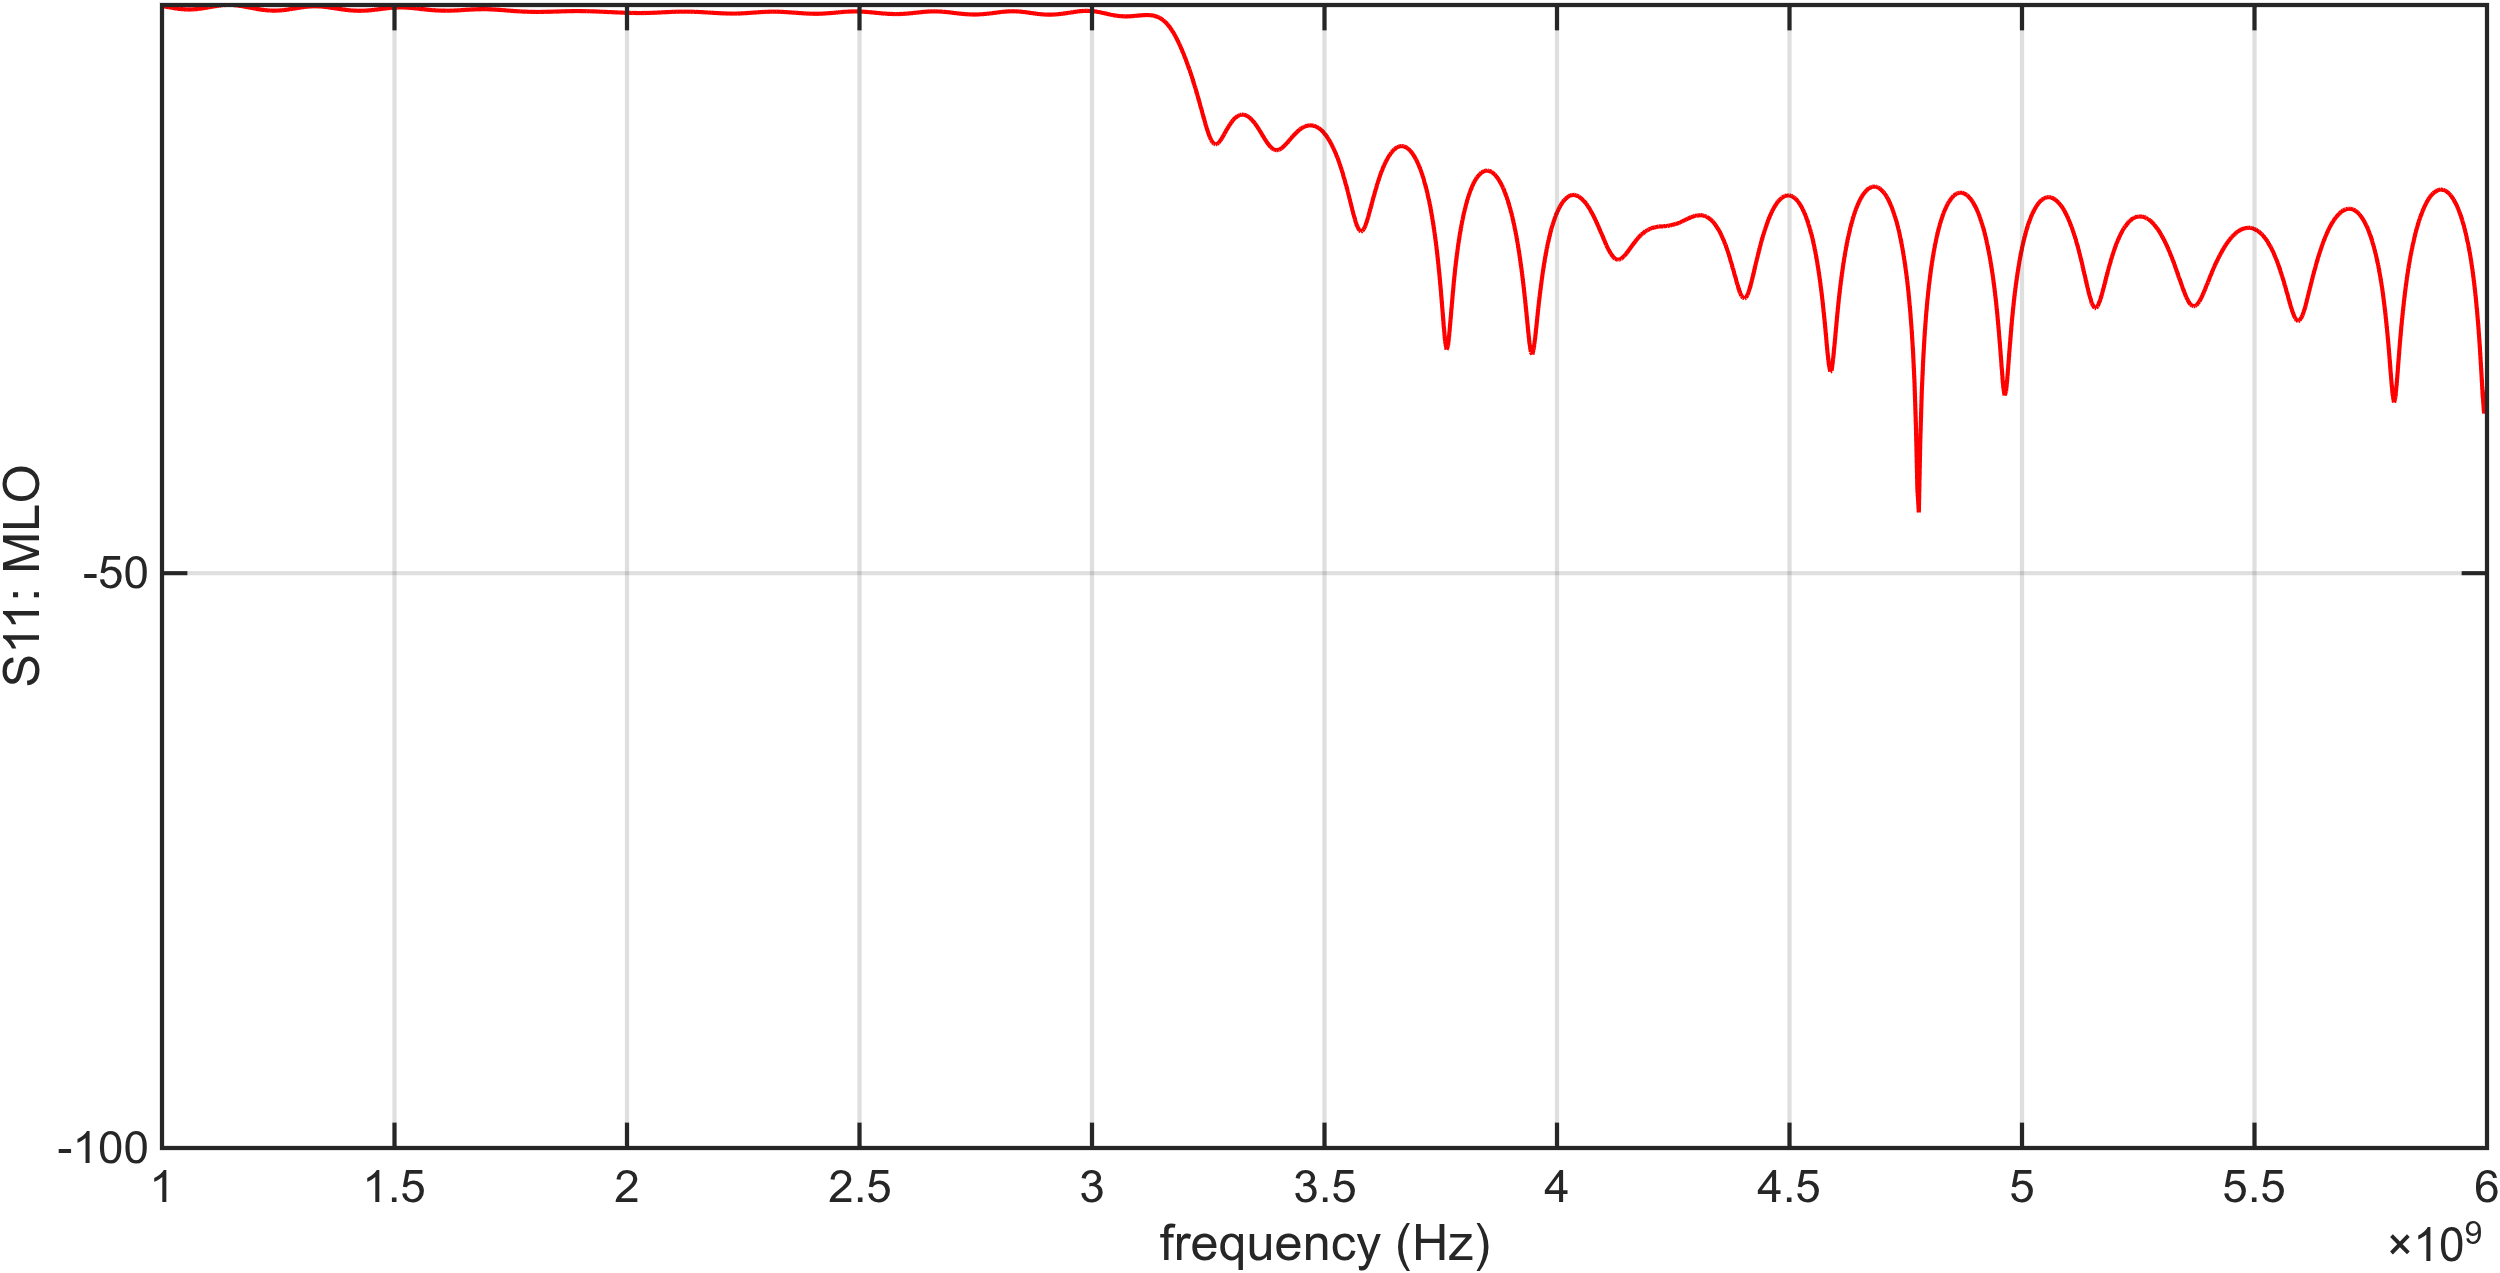
\includegraphics[width=0.6\textwidth]{./Images/Relazione1_Foto/8_b_S11_adattato_per_guida_rect.png}
  \caption{Grafico del coefficiente di riflessione della guida con carico adattato.}
\end{figure}
L'SWR si ricava dalla seguente relazione (con $S_{11}$ in lineare); il grafico è il seguente:
\begin{equation}
  \mathrm{SWR} = \frac{1 + |\Gamma|}{1 - |\Gamma|}= \frac{1 + |S_{11}|}{1 - |S_{11}|}
\end{equation}
\begin{figure}[H]
  \centering
  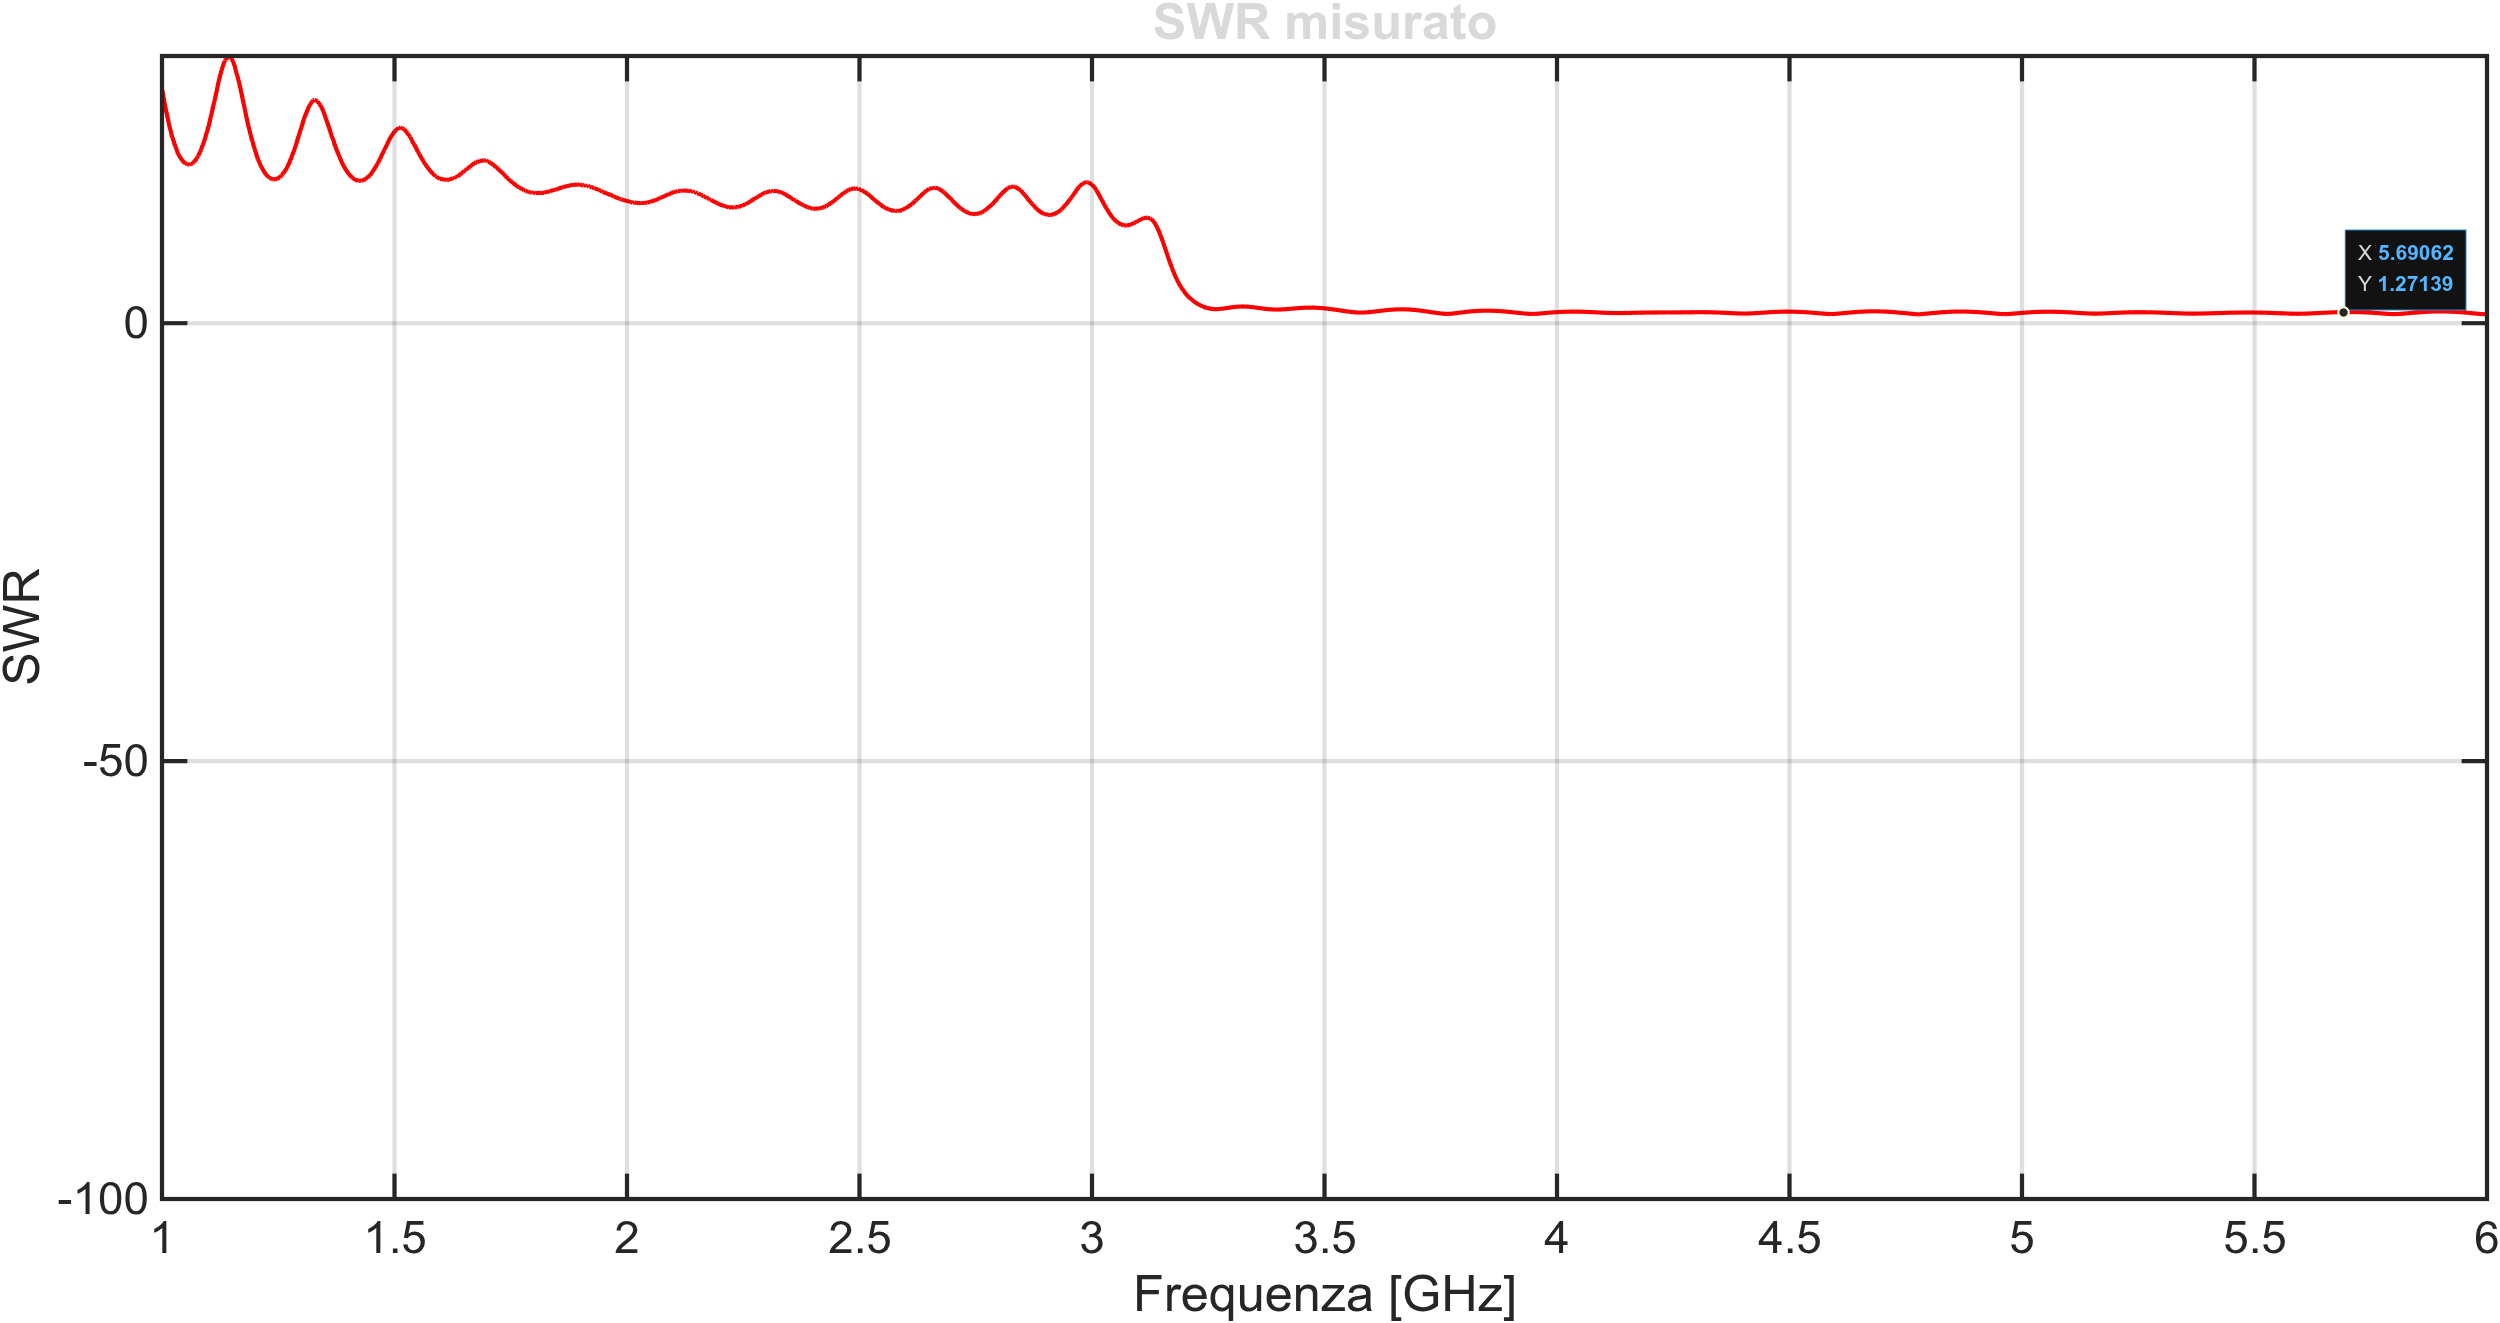
\includegraphics[width=0.6\textwidth]{./Images/Relazione1_Foto/8_c_swr.png}
  \caption{Grafico di SWR in funzione della frequenza.}
\end{figure}
Come si può notare, nella banda del modo TE10, il coefficiente di riflessione assume valori molto piccoli, come ci aspettavamo,
e di conseguenza il valore di SWR tende a 1, come risulta effettivamente dalla misurazione.

% =====================================================================
% Capitolo 9
% =====================================================================
\chapter{Linea di ritardo (delay line)}
\section{Misura della banda della linea}
Per prima cosa abbiamo valutato la banda della linea di ritardo vedendo quando il segnale scende di 3dB, e come si vede
dal grafico accade a circa 55MHz.
\begin{figure}[H]
  \centering
  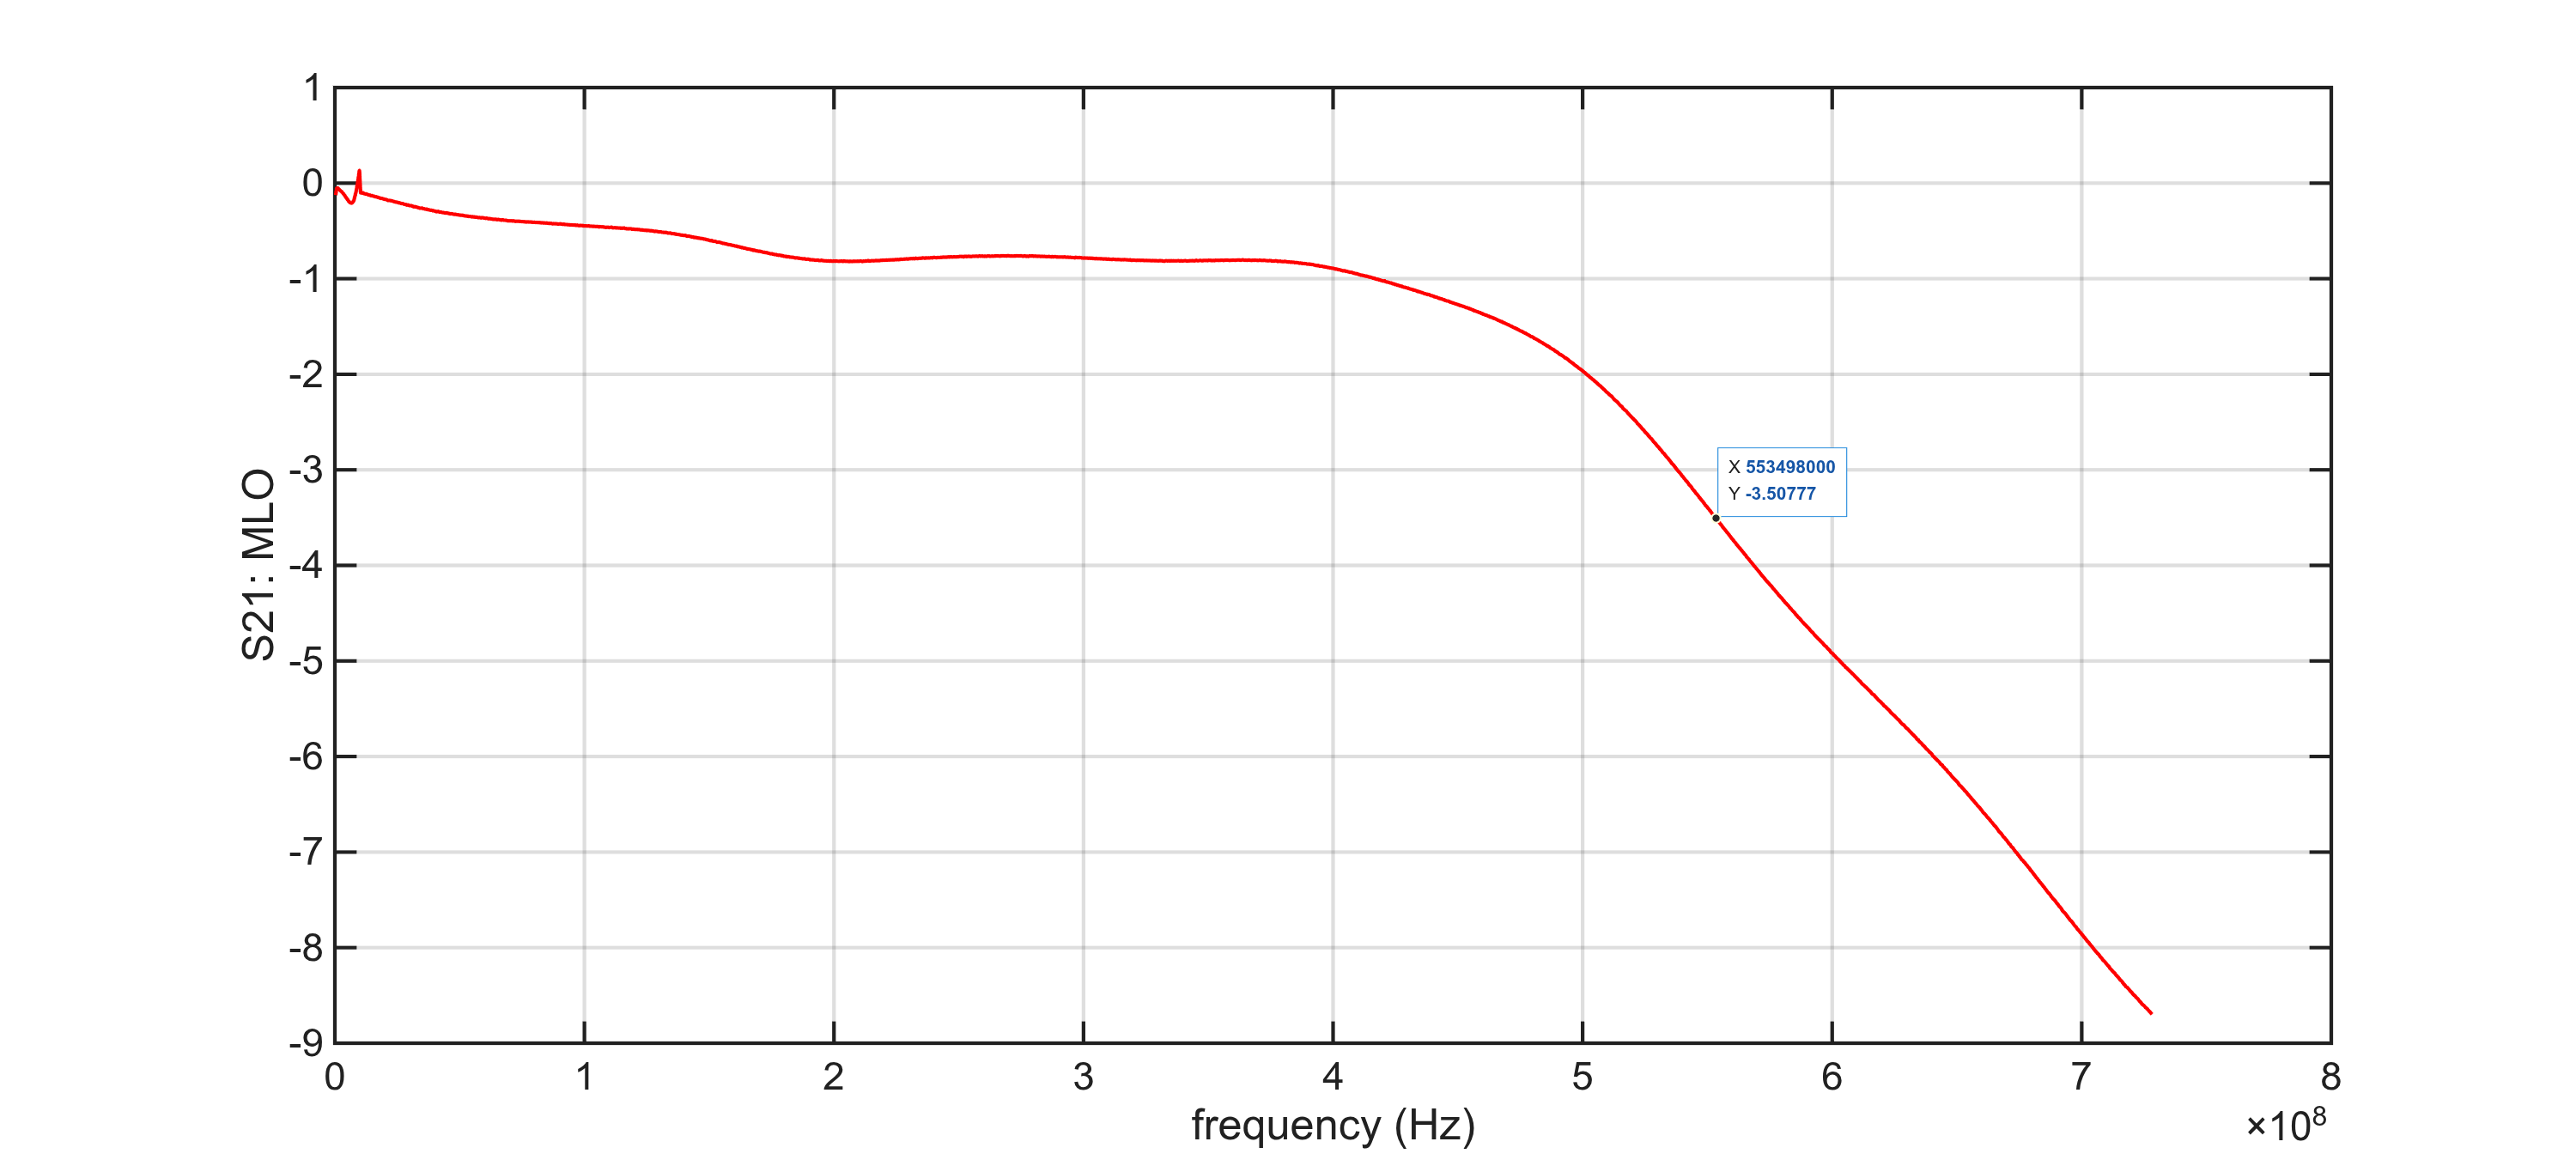
\includegraphics[width=0.6\textwidth]{./Images/Relazione1_Foto/9_1_risposta_linea.png}
  \caption{Andamento in frequenza della delay line, con banda a -3dB.}
\end{figure}
\section{Misura del ritardo massimo}
Una volta valutata la banda passiamo a valutare il ritardo a partire dalla misura di fase con linear fit.
Ricordiamo che la linea di ritardo ha la vite completamente svitata, quindi ci troviamo nel caso di ritardo massimo.
\begin{figure}[H]
  \centering
  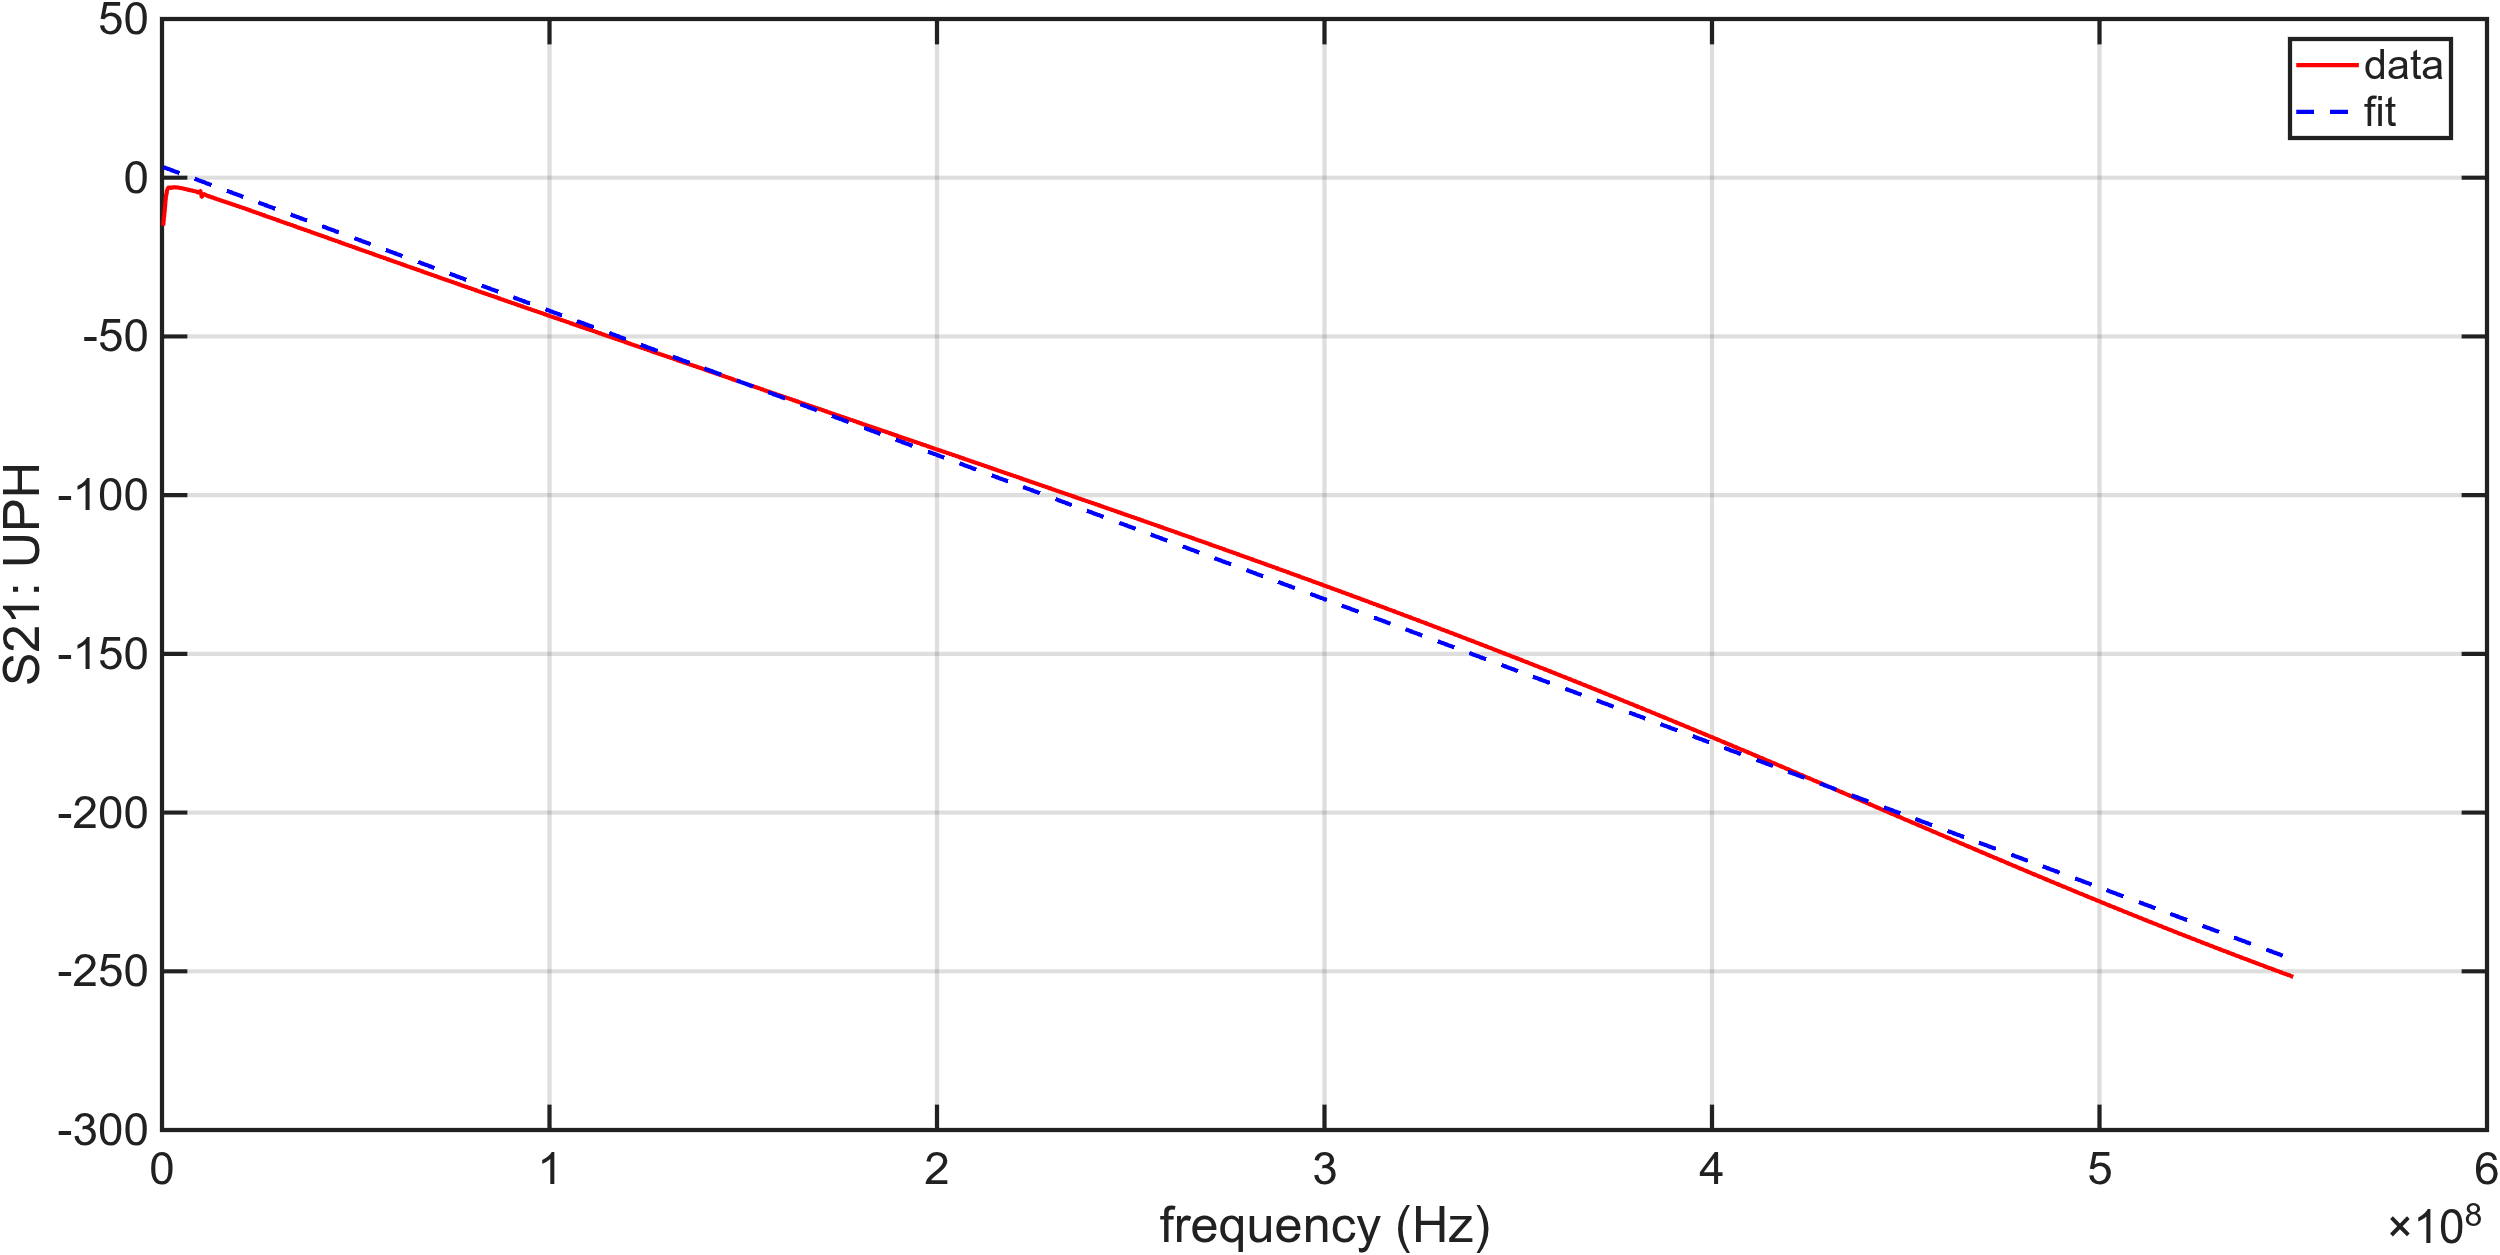
\includegraphics[width=0.6\textwidth]{./Images/Relazione1_Foto/9_2_delay_con_fit.png}
  \caption{Misura della fase di $S_{21}$ con linear fit.}
\end{figure}
Dal linear fit abbiamo una pendenza $ -4.5419 \cdot 10^{-7}$°/Hz e una $\sigma_p = 5.005631105905910 \cdot 10^{-10}$°/Hz.

Dalla pendenza troviamo il ritardo elettrico come nei capitoli precedenti:
\begin{equation}
  \tau_m= \frac{-p(deg)}{360}= 1.2616 \cdot 10^{-9}\ \mathrm{s}
\end{equation}
\begin{equation}
  \tau= [1,2616 \pm 0,0014]\ ns 
\end{equation}
Un altro metodo per valutare il ritardo della linea è tramite l'aggiunta di un ritardo elettrico che annulli la fase.

Nel nostro caso questo accade per un ritardo $\tau=1.22ns$, un valore prossimo a quello valutato con il metodo precedente.

\begin{figure}[H]
  \centering
    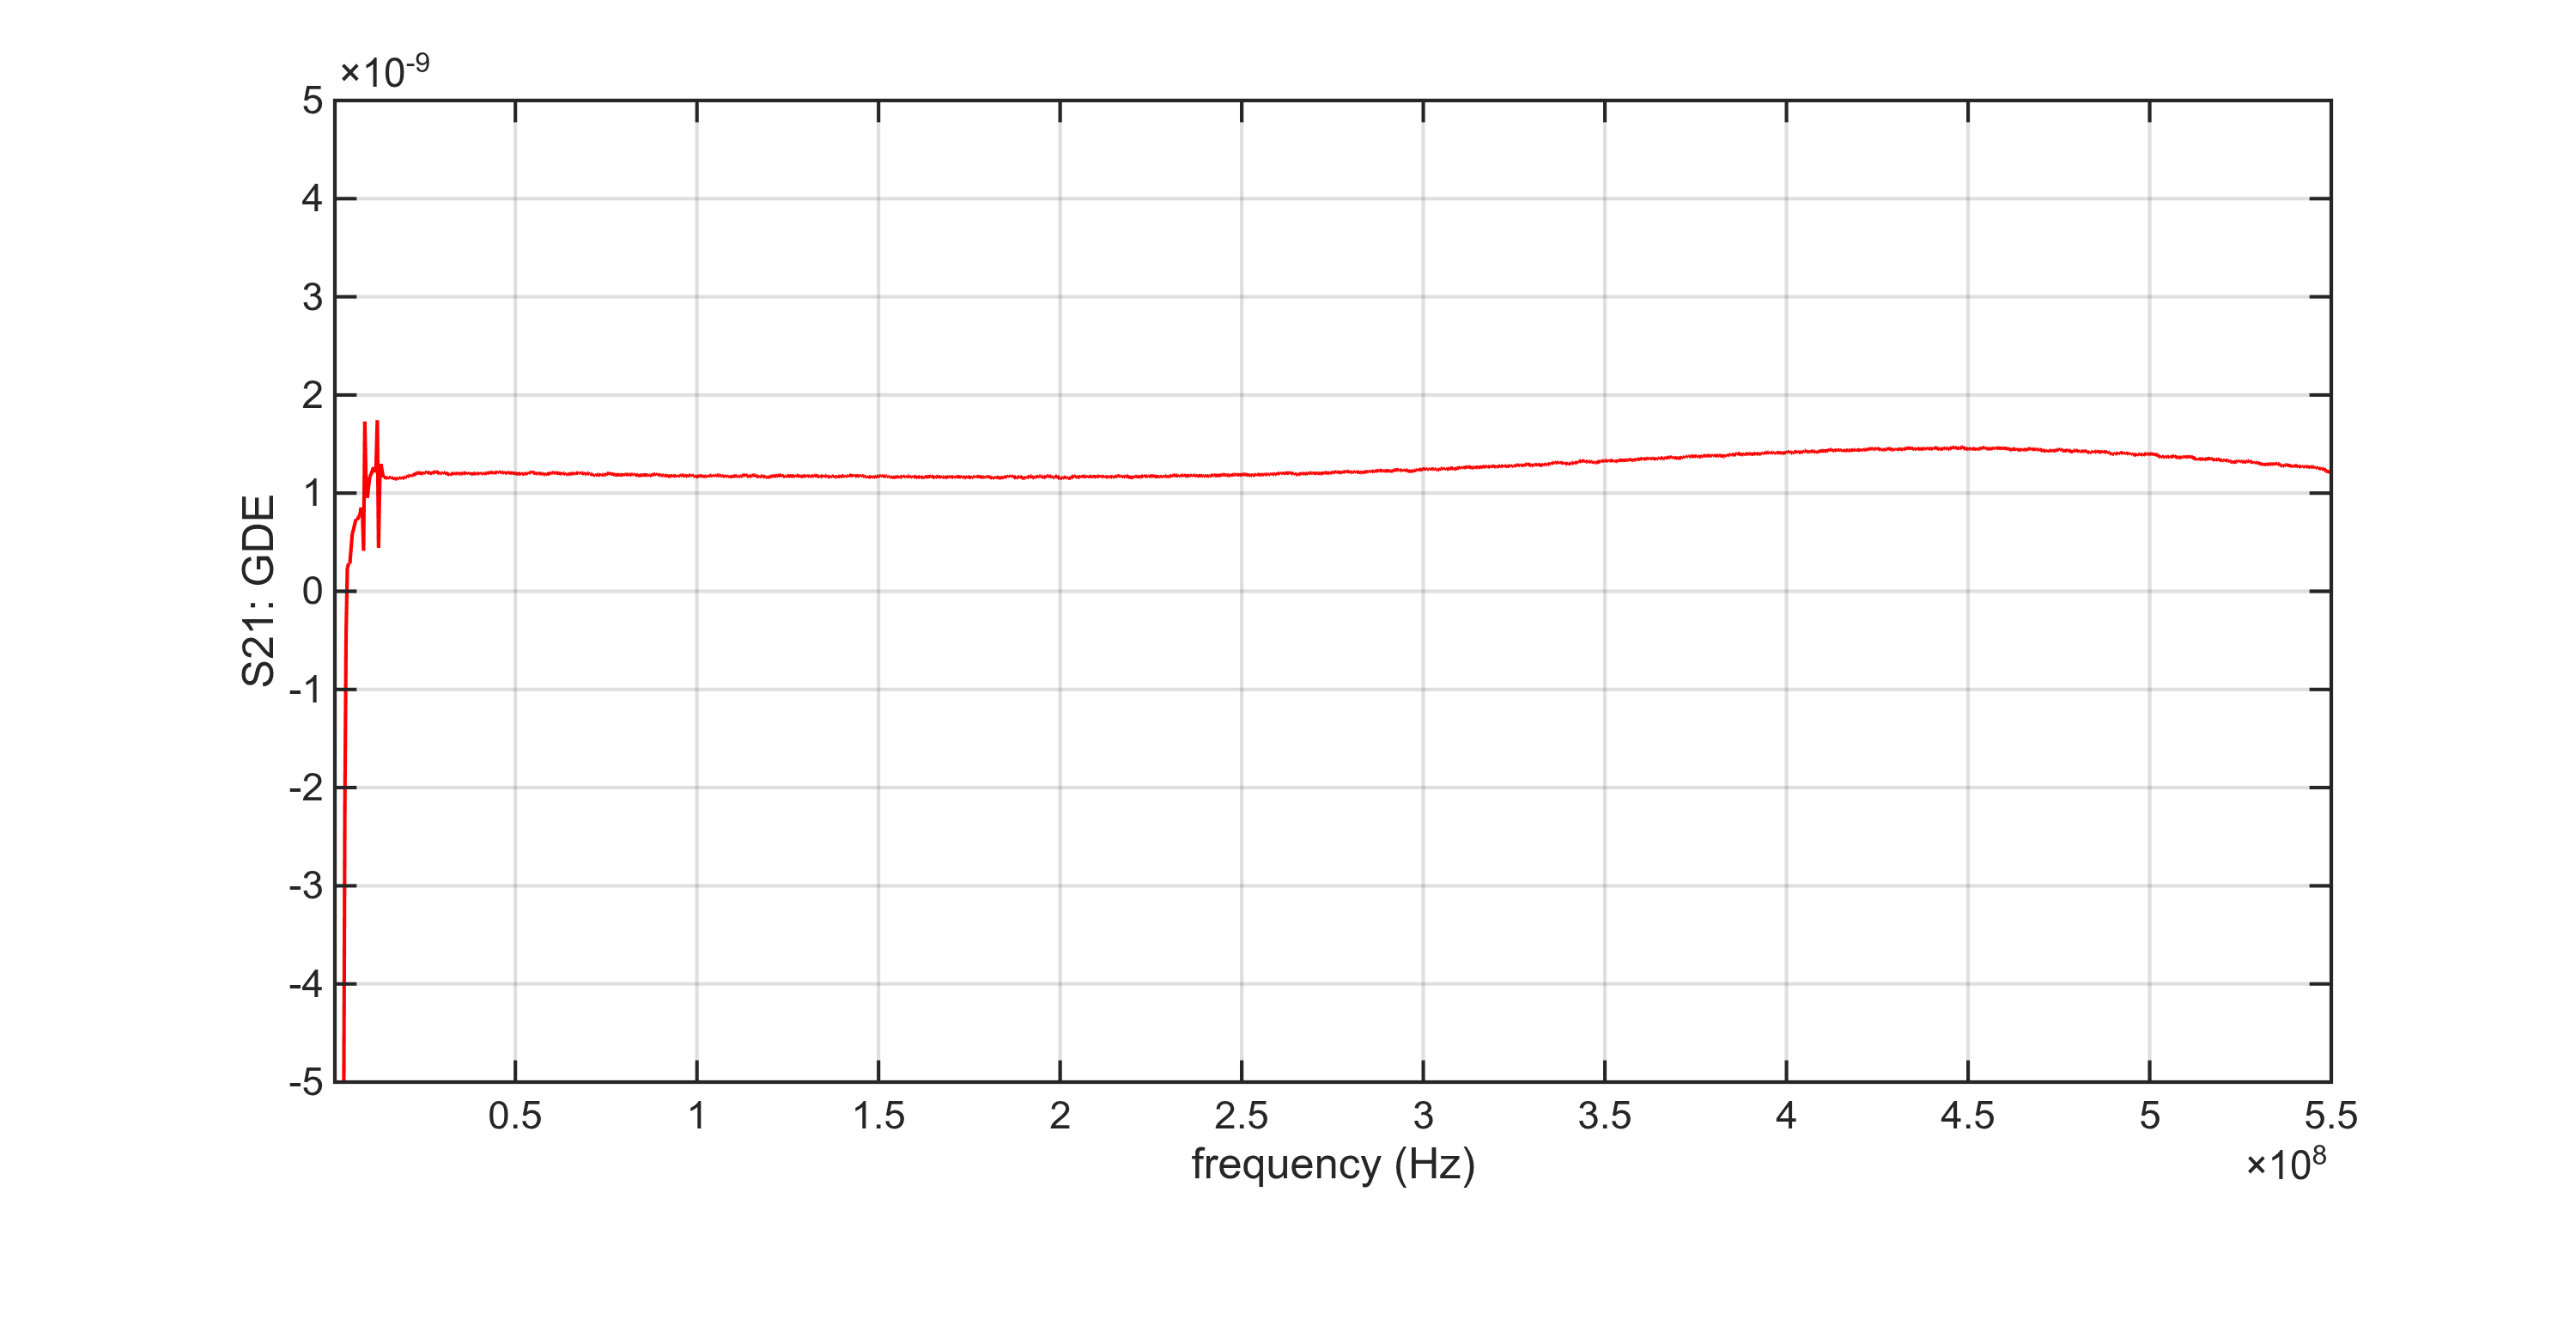
\includegraphics[width=0.6\textwidth]{./Images/Relazione1_Foto/9_3_delay.png}
        \caption{Grafico della fase di $S_{21}$ con electrical delay per ritardo massimo.}

\end{figure}

\section{Misura del ritardo minimo}
In questo caso prendiamo la misura del ritardo della linea con lo stesso metodo del paragrafo precedente ma con la vite completamente avvitata,
quindi con il ritardo minimo. In questo caso l'electrical delay è di 1.12 ns.

\begin{figure}[H]
  \centering
    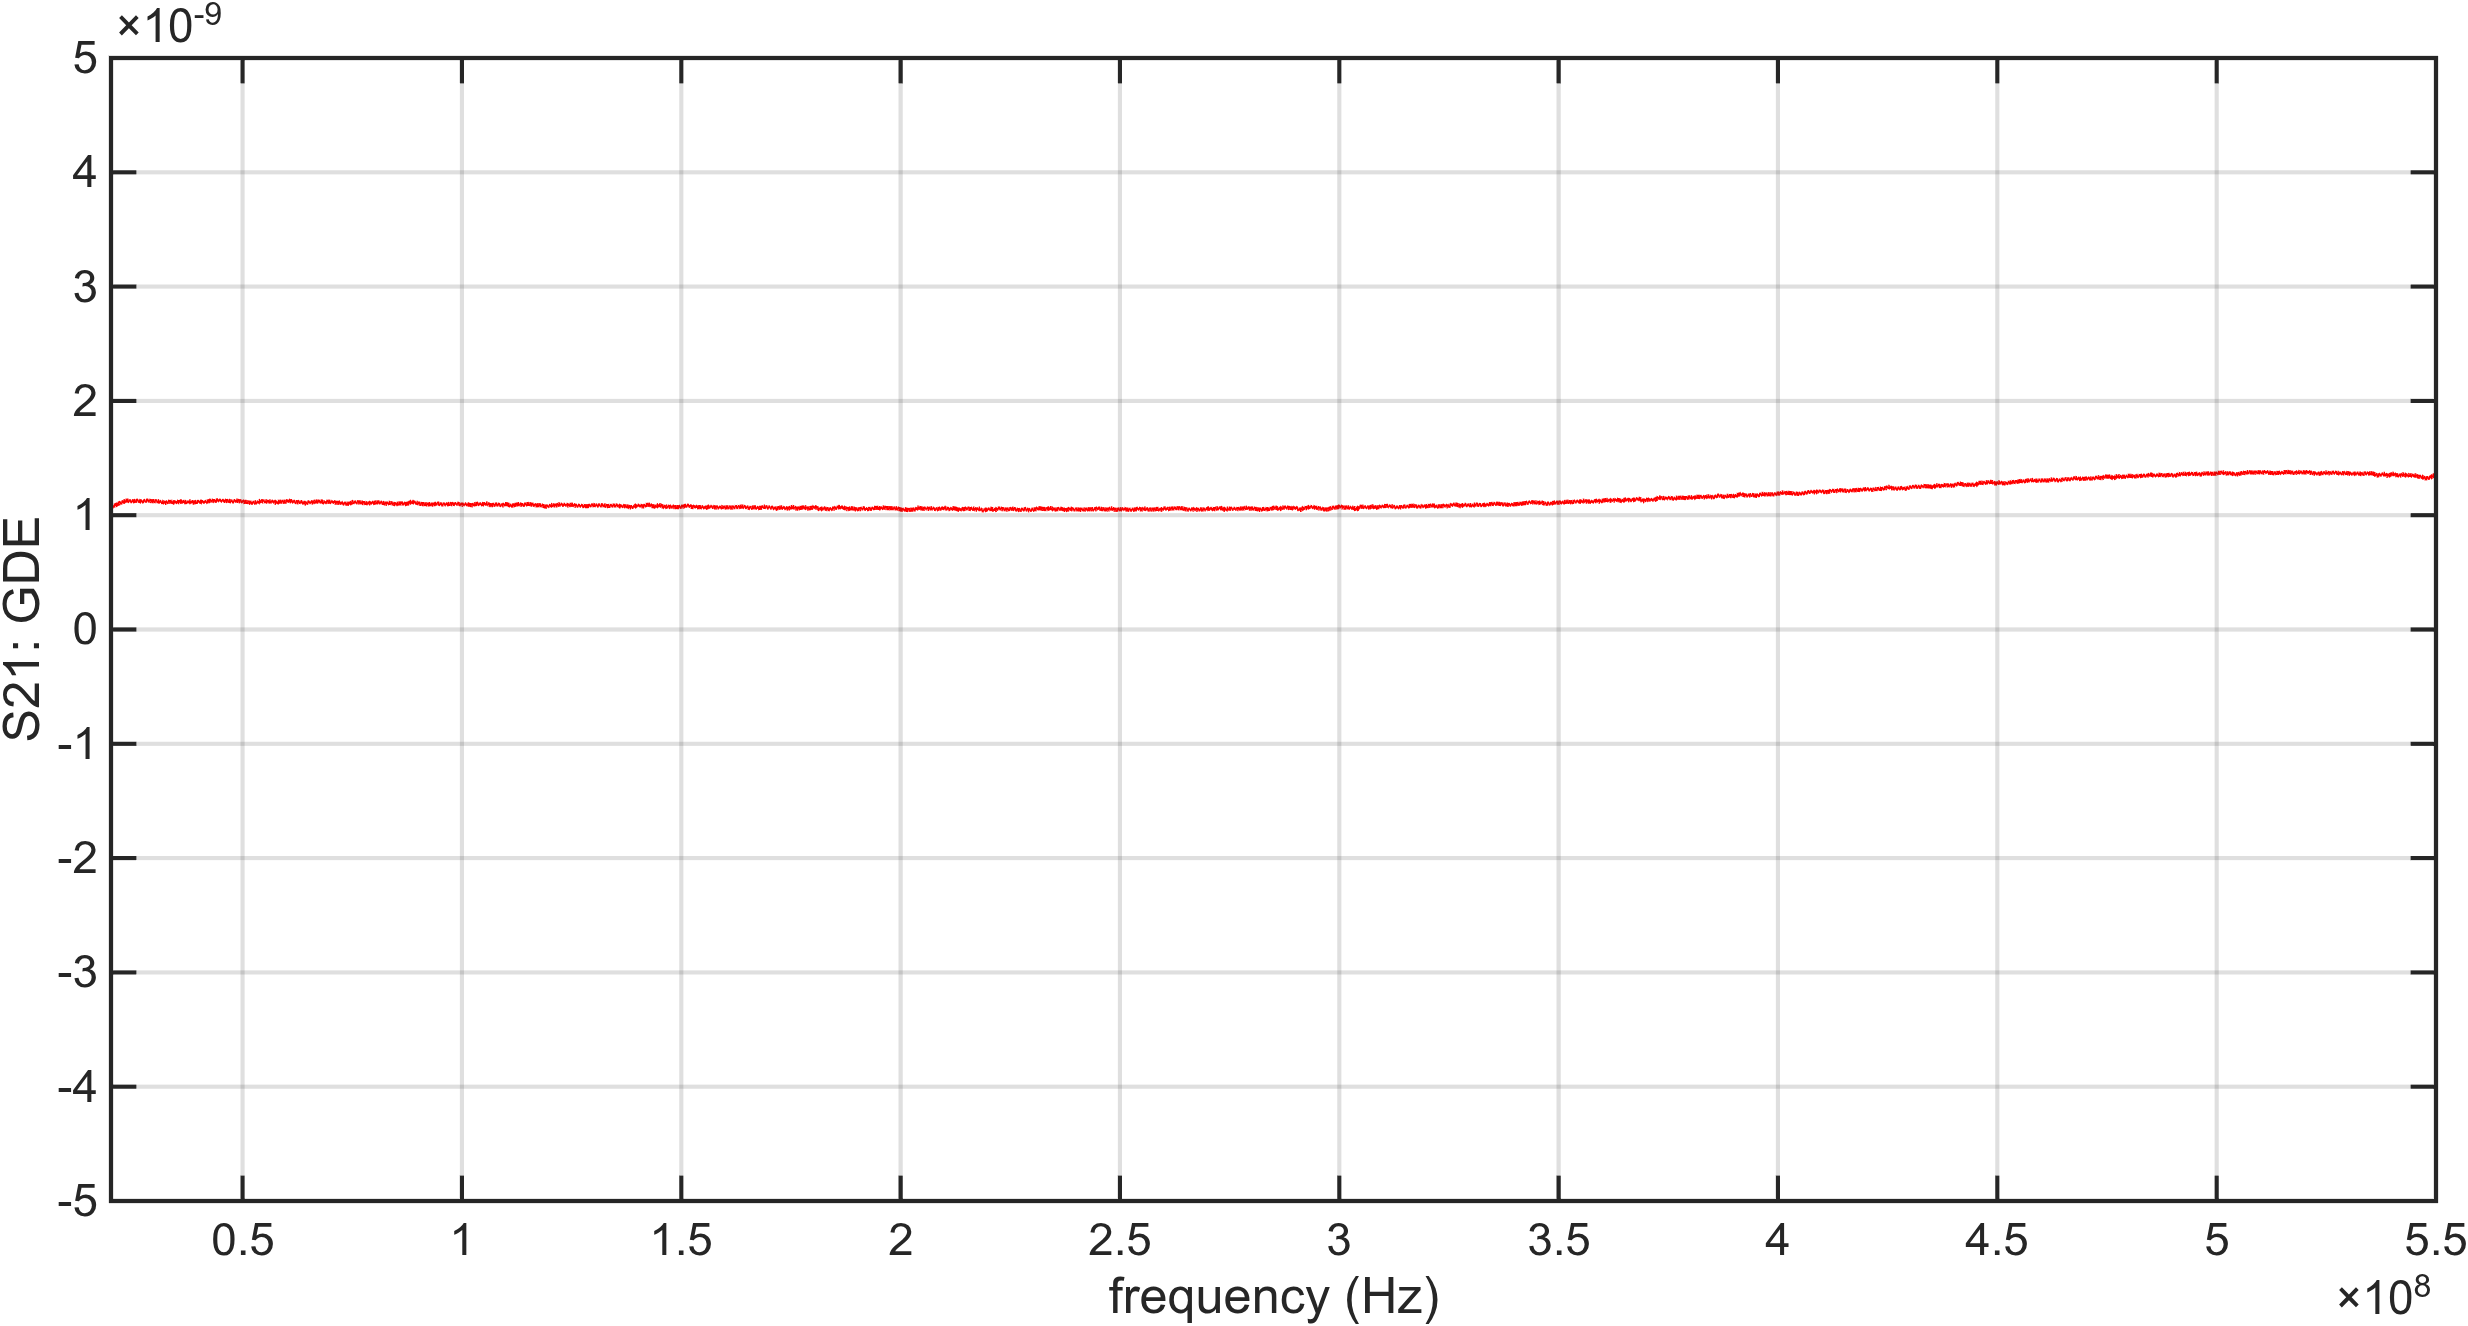
\includegraphics[width=0.6\textwidth]{./Images/Relazione1_Foto/9_3_delay2.png}
    \caption{Grafico della fase di $S_{21}$ con electrical delay per ritardo minimo.}
\end{figure}

\end{document}
9